\documentclass{rapportCS}
\usepackage{lipsum}
\usepackage{booktabs}
\usepackage[utf8]{inputenc}
\usepackage[english]{babel}
\usepackage{amsmath, amssymb}
\usepackage{graphicx}
\usepackage{float}
\usepackage{caption}
\usepackage{subcaption}
\usepackage{geometry}
\geometry{margin=3cm}
\usepackage{listings}
\usepackage{hyperref}
\title{Control Theory Report} %Titre du fichier

\begin{document}

%----------- Informations du rapport ---------

\logoentreprise{logos/parissaclay.png}

\titre{Speed Control of an Electrical Drive} % Title
\soustitre{Vitesse - Track A - Trinome 32}

\eleve{Jin DING \\
Carlos BENÍTEZ ROSETY \\
Marcos Ichiro SASAKI}

\infocours{TP Report \\ Control Theory}

\dates{19/09/2025 - 22/10/2025}

%----------- Initialisation -------------------
        
\fairemarges %Afficher les marges
\fairepagedegarde %Créer la page de garde

%----------- Abstract -------------------
\vspace*{\stretch{1}}
\begin{center}
	\begin{abstract}
        This practical work focuses on the modeling, control, and experimental validation of a DC electrical drive system. The objective was to design and implement cascaded control strategies capable of regulating the motor’s speed and current with high precision. The study began with the identification of the motor’s electrical and mechanical parameters — including resistance, inductance, torque and voltage constants, friction coefficients, and moment of inertia — which provided the foundation for accurate system modeling.

A two-level control structure was developed: an inner current loop designed via pole placement to achieve fast and stable current regulation, and an outer speed loop tuned using both linear quadratic (LQ) and proportional control strategies. An observer was then implemented to estimate unmeasured variables such as speed and load torque, improving disturbance rejection and enabling feed-forward compensation.

Simulations were performed in MATLAB/Simulink to validate the theoretical designs under various operating conditions, including load disturbances and setpoint variations. The experimental implementation confirmed the robustness of the controllers, demonstrating low overshoot, minimal steady-state error, and good dynamic performance. The observer-based compensation was also evaluated, showing effective convergence in simulation and practical limitations due to measurement noise.

Overall, the project successfully bridged theoretical control design with real-world application, illustrating the integration of modeling, simulation, and experimental testing in modern electromechanical systems.
    \end{abstract}
\end{center}
\vspace*{\stretch{1}}
\newpage

%------------ Table des matières ----------------

\tabledematieres % Créer la table de matières

%------------ Corps du rapport ----------------


%------------ Section 1 ----------------

\section{Identification of the System Parameters}

\subsection{Introduction}

The objective of this practical work is to design and implement control strategies for the speed regulation of a direct current (DC) electrical drive system. Such systems are widely used in transportation, robotics, and industrial automation, where precise speed control ensures efficiency and reliability.

The study combines modeling, simulation, and experimentation. First, the electrical and mechanical parameters of the DC motor are identified using a platform composed of two coupled DC machines, sensors, and a DC/DC converter. Then, controllers are designed and validated in Matlab/Simulink—an inner current loop by pole placement and an outer speed loop using a linear quadratic (LQ) approach. Finally, the controllers are tested on the physical setup to compare real and simulated performances.

Part 1 focuses on parameter identification, determining key characteristics such as resistance, inductance, torque and voltage constants, friction coefficients, and inertia. These parameters provide the foundation for accurate modeling and effective control design in the subsequent stages.

\vspace{1em}
\noindent The equations governing the DC motor system are as follows:
\begin{align}
U_m(t) &= R \cdot I(t) + L \frac{dI(t)}{dt} + E(t) \label{eq:voltage} \\
E(t) &= K_e \cdot \Omega(t) \label{eq:bemf} \\
C_e(t) &= K_c \cdot I(t) \label{eq:torque} \\
C_e(t) &= C_r(t) + C_s + f \cdot \Omega(t) + J \frac{d\Omega(t)}{dt} \label{eq:mechanical}
\end{align}

\noindent where:
\begin{itemize}
    \item $R$: armature resistance ($\Omega$)
    \item $L$: armature inductance (H)
    \item $E$: counter-electromotive force of the motor (V)
    \item $\Omega$: rotational speed of the rotor (rad $\cdot$ s$^{-1}$)
    \item $C_e$: electromagnetic torque of the motor (N $\cdot$ m)
    \item $K_e$: voltage constant (V $\cdot$ s)
    \item $K_c$: torque constant (N $\cdot$ m $\cdot$ A$^{-1}$)
    \item $C_r$: resistant torque (N $\cdot$ m)
    \item $C_s$: Coulomb friction torque (N $\cdot$ m)
    \item $f$: viscous friction coefficient (N $\cdot$ m $\cdot$ s)
    \item $J$: moment of inertia of the shafts of the two machines (kg $\cdot$ m$^2$)
\end{itemize}

\subsection{Armature Resistance and Inductance: $R$ and $L$}

The armature resistance ($R$) and inductance ($L$) characterize the electrical behavior of the DC motor’s armature circuit. The resistance $R$ represents the opposition to the flow of current in the winding, while the inductance $L$ reflects the ability of the winding to store energy in its magnetic field. These parameters directly influence the transient response of the current when a voltage is applied to the motor.

To determine $R$ and $L$, the rotor is kept stationary so that no back electromotive force (EMF) is generated. A step voltage $u_c(t)$ of $2.5\,\mathrm{V}$ is applied through the DC/DC converter, and the corresponding current response is observed in the Simulink oscilloscope. The experiment can be modeled as a simple first-order RL circuit governed by:

\[
U_m(t) = R I(t) + L \frac{dI(t)}{dt}.
\]

At steady state, the current reaches a constant value $I_\infty$, allowing the armature resistance to be calculated as:

\[
R = \frac{U_m}{I_\infty}.
\]

The inductance $L$ is obtained from the electrical time constant $\tau_e$ of the current response, given by:

\[
\tau_e = \frac{L}{R} \quad \Longrightarrow \quad L = R \cdot \tau_e.
\]

The measured quantities during the experiment are summarized in Table~\ref{tab:RLvalues}.

\begin{table}[H]
\centering
\caption{Measured and calculated values for $R$ and $L$}
\label{tab:RLvalues}
\begin{tabular}{lccc}
\toprule
\textbf{Quantity} & \textbf{Symbol} & \textbf{Measured Value} & \textbf{Unit} \\
\midrule
Applied voltage & $V$ & 6.5 & V \\
Steady-state current & $I$ & 18.55 & A \\
Electrical time constant & $\tau_e$ & 0.025 & s \\
\midrule
Calculated resistance & $R$ & 0.3504 & $\Omega$ \\
Calculated inductance & $L$ & 0.00876 & H \\
\bottomrule
\end{tabular}
\end{table}

\begin{figure}[H]
\centering
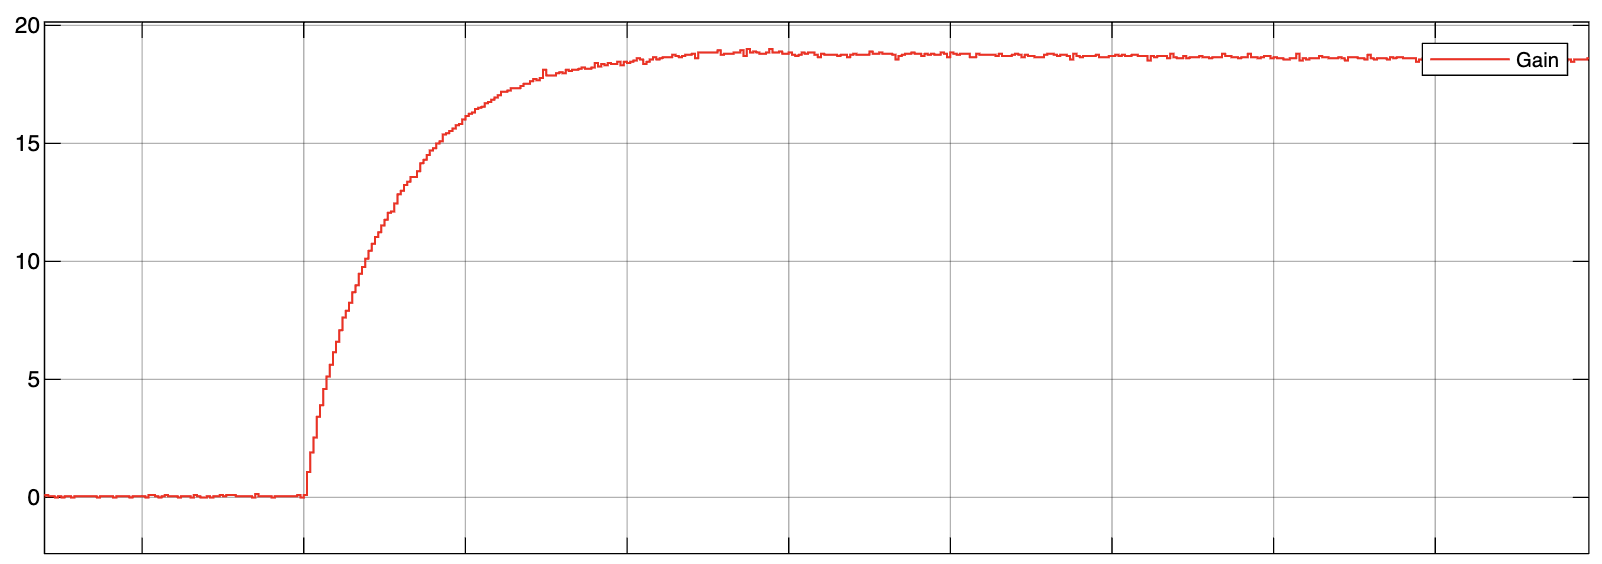
\includegraphics[width=0.7\textwidth]{figures/graph_i_time.png}
\caption{Current response $I(t)$ to step voltage input, showing the transient behavior and steady-state value.}
\label{fig:i_time}
\end{figure}

Thus, from the steady-state and transient measurements, the armature resistance and inductance of the DC machine were found to be:

\[
R = 0.3504~\Omega, \qquad L = 0.00876~\mathrm{H}.
\]

These values will be used in subsequent stages for the modeling and control design of the electrical drive system.

\subsection{Voltage Constant and Torque Constant: $K_e = K_c$}

In steady state, the armature voltage satisfies
\[
U_m = E + R\,I = K_e\,\Omega + R\,I,
\]
so the (back–EMF) voltage constant $K_e$ (equal to the torque constant $K_c$ in SI units) can be obtained directly from averaged steady-state measurements as
\[
K_e \;=\; \frac{\overline{U}_m - R\,\overline{I}}{\overline{\Omega}} \qquad (\text{with } \overline{\Omega}\text{ in rad/s}).
\]


\paragraph{}
With the rotor turning (stator energized), we applied a constant control $u_c$ at the converter input and increased it in steps $u_c=0,2,3,4~\mathrm{V}$, waiting for steady state each time. At steady state we recorded:
(i) the average armature voltage $U_m$ (voltmeter),
(ii) the current sensor output $V_I$ (converted to $I$ via $I=V_I/K_{\mathrm{cap}I}$ with $K_{\mathrm{cap}I}=0.1~\mathrm{V/A}$),
and (iii) the rotational speed in rpm (converted to $\Omega$ via $\Omega= \text{rpm}\cdot 2\pi/60$).

\paragraph{}
\begin{table}[H]
\centering
\caption{Steady-state measurements and converted quantities.}
\label{tab:Ke_data}
\begin{tabular}{lccccc}
\toprule
$u_c$ (V) & $V_I$ (V) & rpm & $\Omega$ (rad/s) & $I=V_I/0.1$ (A) & $U_m$ (V)\\
\midrule
0 & 0.0374 & 3.0184  & 0.316086 & 0.374  & 0 \\
2 & 0.9976 & 57.1736 & 5.987205 & 9.976  & 5 \\
3 & 1.1536 & 184.3761& 19.307820& 11.536 & 16 \\
4 & 1.2517 & 317.6292& 33.262052& 12.517 & 27 \\
\bottomrule
\end{tabular}
\end{table}

Using the previously identified armature resistance
\[
R = 0.350404313~\Omega,
\]
and the averaged values from our measurements (already converted to SI units):
\[
\overline{U}_m = 12~\text{V},\quad
\overline{I} = 0.860075~\text{A},\quad
\overline{\Omega} = 14.7182909~\text{rad/s} \;\;(\text{from } 140.549325~\text{rpm}),
\]
we obtain
\[
K_e \;=\; \frac{12 - 0.350404313 \times 0.860075}{14.7182909}
\;=\; 0.794835901~\text{V}\cdot\text{s/rad}.
\]

Hence, in SI units,
\[
\boxed{\,K_e = K_c \approx 0.794835901~\text{V}\cdot\text{s/rad}\,}.
\]

\subsection{Coulomb Friction Torque and Viscous Friction Coefficient: $C_s$ and $f$}

In steady state (constant speed, $\dot{\Omega}=0$) and with zero external load torque ($C_r=0$), the DC motor torque balance reduces to
\[
K_c\,I \;=\; f\,\Omega \;+\; C_s ,
\]
where $K_c$ is the torque constant (equal to the back–EMF constant in SI), $f$ is the viscous friction coefficient, and $C_s$ is the Coulomb (dry) friction torque.

Hence, plotting the measured current $I$ versus angular speed $\Omega$ and fitting the affine model
\[
I \;=\; a\,\Omega \;+\; b
\]
yields $f = K_c\,a$ and $C_s = K_c\,b$.

\paragraph{}
\begin{table}[H]
\centering
\caption{Steady-state points used for $I$–$\Omega$ identification.}
\label{tab:friction_data}
\begin{tabular}{lcccc}
\toprule
$u_c$ (V) & $U_m$ (V) & rpm & $\Omega$ (rad/s) & $I$ (A)\\
\midrule
2 & 5  & 57.1736  & 5.987205 & 0.9976 \\
3 & 16 & 184.3761 & 19.307820 & 1.1536 \\
4 & 27 & 317.6292 & 33.262052 & 1.2517 \\
6 & 49 & 593.3711 & 62.137676 & 1.6074 \\
\bottomrule
\end{tabular}
\end{table}

A linear regression of $I$ vs.\ $\Omega$ gives (see plotted trendline):
\[
I \;=\; \underbrace{0.0107}_{a}\,\Omega \;+\; \underbrace{0.9293}_{b}\quad [\mathrm{A}],
\]
with $\Omega$ in rad/s.

\begin{figure}[H]
\centering
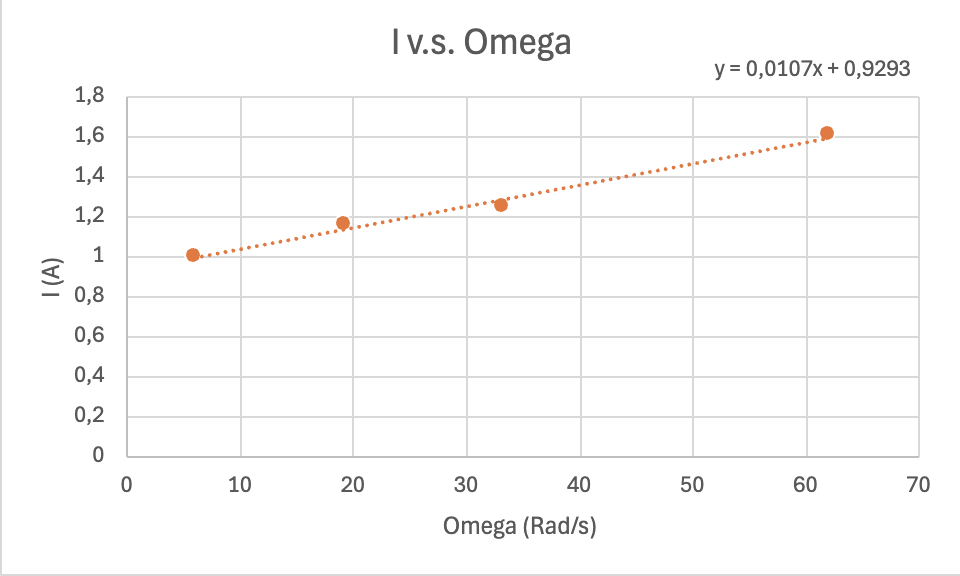
\includegraphics[width=0.7\textwidth]{figures/graph_i_omega.png}
\caption{Linear regression of steady-state current $I$ versus angular speed $\Omega$.}
\label{fig:i_omega}
\end{figure}

Using the previously identified $K_c = K_e = 0.794835901~\mathrm{V\,s/rad} = \mathrm{N\,m/A}$, we obtain
\[
f \;=\; K_c\,a \;=\; 0.794835901 \times 0.0107 \;=\; \mathbf{0.008504744}~\mathrm{N\,m\,s},
\]
\[
C_s \;=\; K_c\,b \;=\; 0.794835901 \times 0.9293 \;=\; \mathbf{0.738641003}~\mathrm{N\,m}.
\]

These friction parameters will be used in the motor model and subsequent controller design/validation.

\subsection{Moment of Inertia of the System: $J$}

When the control signal is removed, the motor supply is cut and the rotor slows down under the effect of friction only. The deceleration obeys
\[
J\,\dot{\Omega}(t) + f\,\Omega(t) + C_s = 0,
\]
or, with $\tau=\tfrac{J}{f}$,
\[
\dot{\Omega}(t) + \frac{1}{\tau}\,\Omega(t) \;=\; -\frac{C_s}{J}.
\]
Its solution for $t\ge 0$ (with $\Omega_0=\Omega(0)$ at switch--off) is
\[
\Omega(t) \;=\; \Big(\Omega_0 + \frac{C_s}{f}\Big)\,e^{-t/\tau} \;-\; \frac{C_s}{f}.
\tag{*}
\]

\begin{figure}[H]
\centering
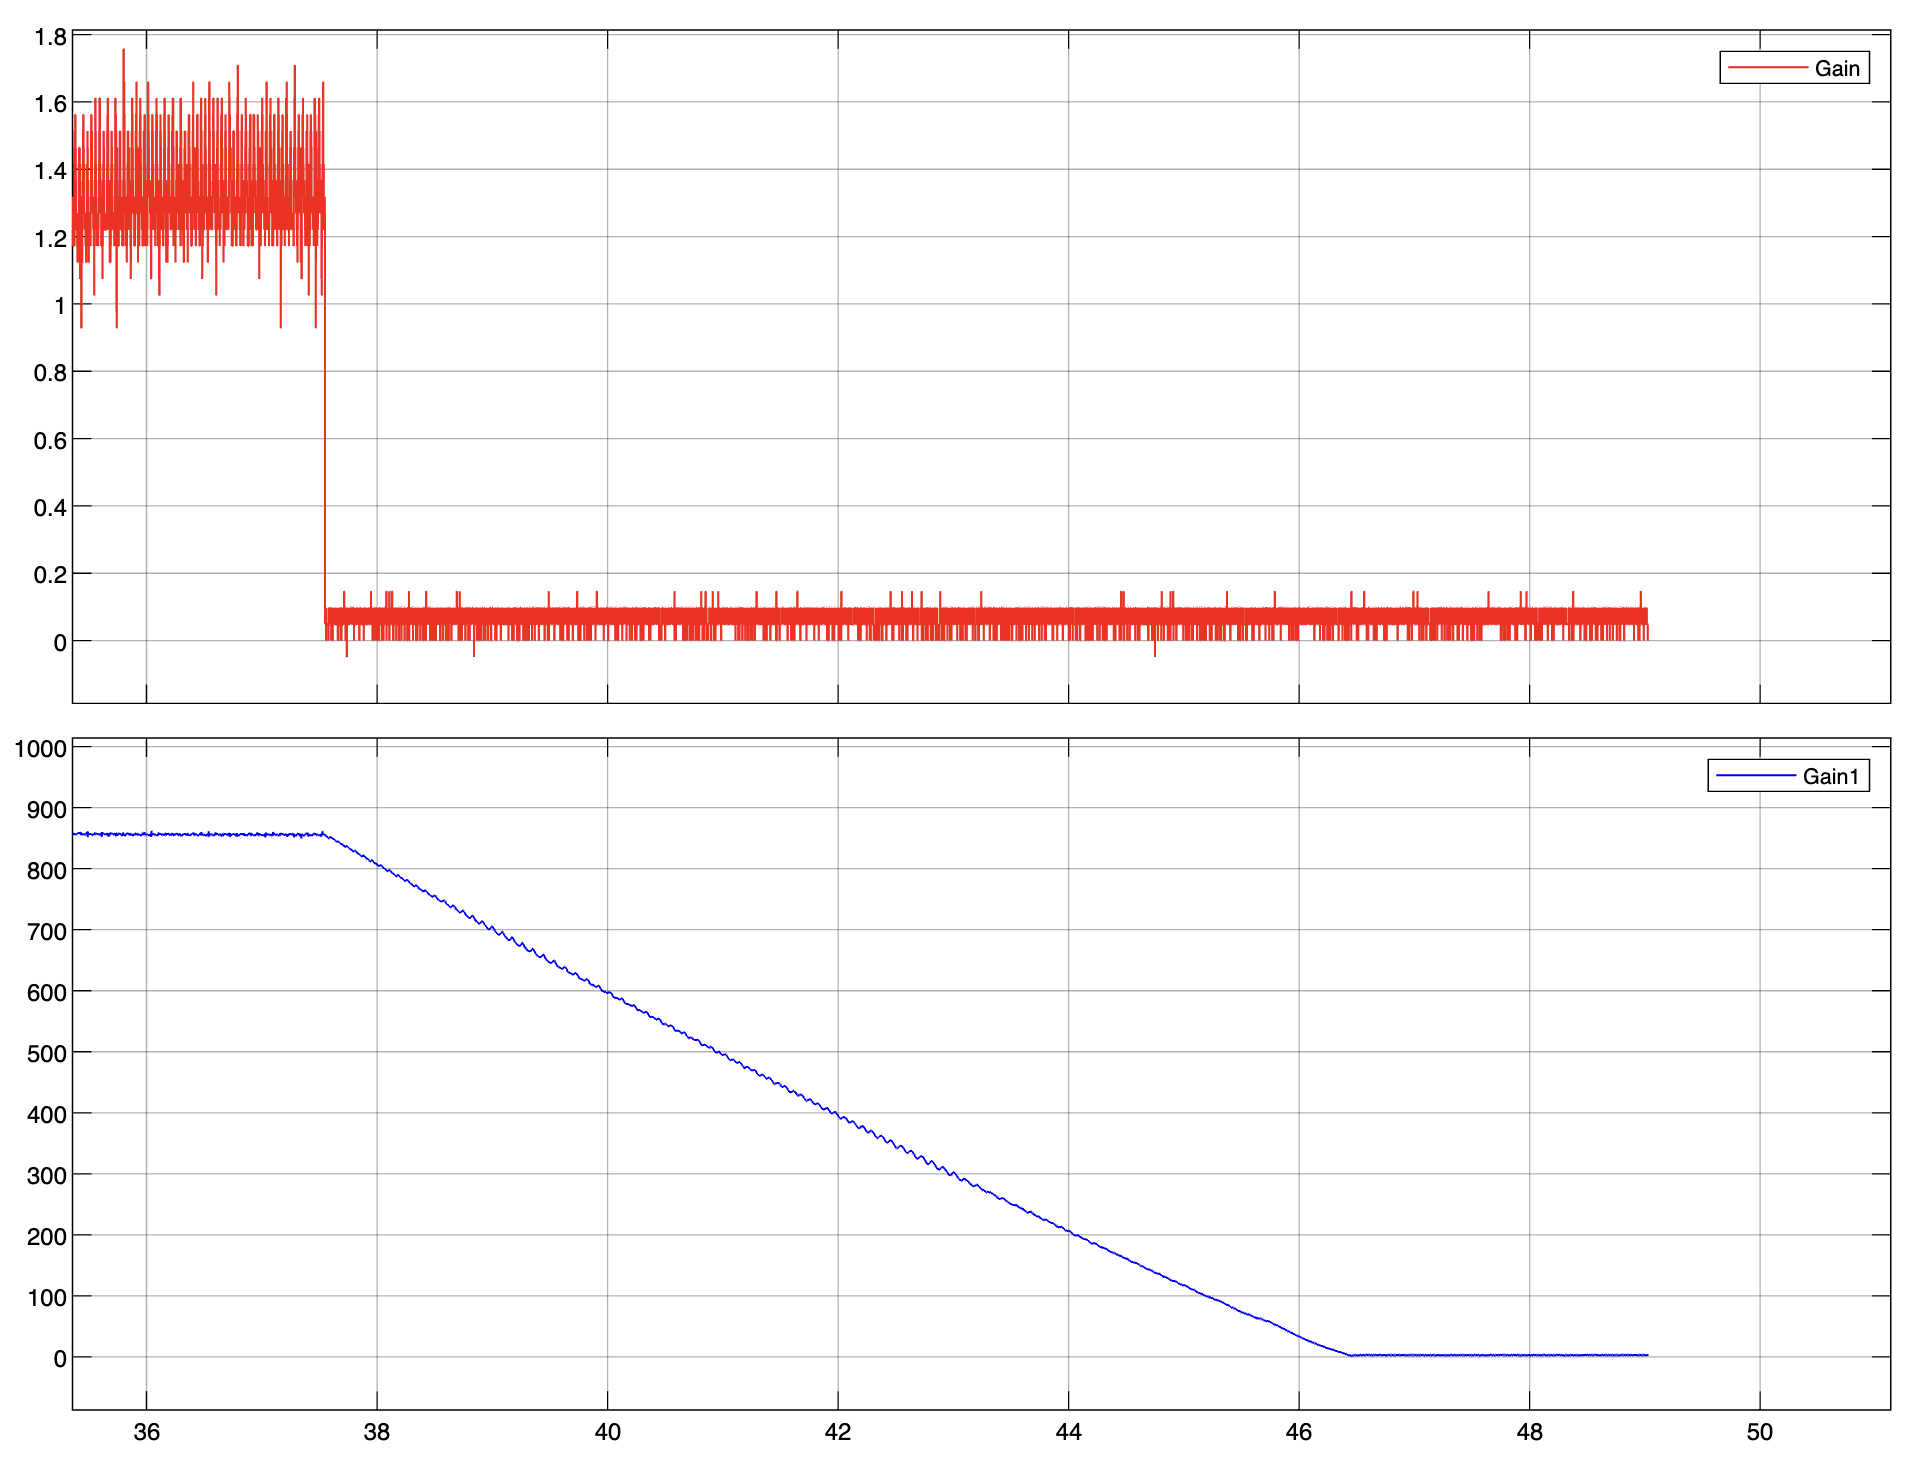
\includegraphics[width=0.7\textwidth]{figures/signal_removed.png}
\caption{Angular velocity $\Omega(t)$ decay (blue curve) after supply cut (Figure~\ref{fig:J_measurement}).}
\label{fig:J_measurement}
\end{figure}

\noindent
We used \textsc{Matlab} code to fit a function that approximates the experimental speed decay curve shown in Figure~\ref{fig:J_measurement}. The fitting process involved nonlinear least squares optimization to match the analytical model \eqref{fig:J_measurement} (equation~(*)) to the measured data, with $\tau$ and $\Omega_0$ as fitting parameters while $f$ and $C_s$ were held constant at their previously identified values. The fitted function closely matches the experimental decay, and from this fitted model we directly obtained the moment of inertia as

\noindent
Using the fitted function parameters, we obtain
\[
\boxed{J = 0.1213266~\mathrm{kg\cdot m^2}}.
\]
This $J$ is used in the subsequent modeling and control design stages.



\newpage
%------------ Section 2 ----------------

\section{Controller Design and Validation by Simulations}

\subsection{Current Regulation}
\subsubsection{State-Space Model of the Augmented System}

The armature circuit of the DC motor is governed by:
\begin{equation*}
U_m(t) = R\,I(t) + L\,\frac{dI(t)}{dt} + K_e\,\Omega(t)
\end{equation*}
and the converter is modeled as:
\begin{equation*}
U_m(t) = k_h\,u_c(t), \qquad k_h = 10
\end{equation*}

Hence, the current dynamics can be written as:
\begin{equation*}
\frac{dI(t)}{dt} = -\frac{R}{L}\,I(t) + \frac{k_h}{L}\,u_c(t) - \frac{K_e}{L}\,\Omega(t)
\end{equation*}

To ensure zero steady-state error, an integral action is introduced through the integral of the current error:
\begin{equation*}
x_{\varepsilon I}(t) = \int_0^t \big(V_{I^*}(\tau) - V_I(\tau)\big)\,d\tau
\end{equation*}
where the current sensor gives:
\begin{equation*}
V_I = K_{\mathrm{conv},I}\,I(t), \qquad K_{\mathrm{conv},I} = 0.1~\text{V/A}
\end{equation*}
Thus:
\begin{equation*}
\frac{dx_{\varepsilon I}(t)}{dt} = V_{I^*}(t) - V_I(t)
\end{equation*}

Define the augmented state vector and the output as:
\begin{equation*}
x_I(t) =
\begin{bmatrix}
I(t) \\[4pt]
x_{\varepsilon I}(t)
\end{bmatrix},
\qquad
y_I(t) = V_I(t) = K_{\mathrm{conv},I}\,I(t)
\end{equation*}

The augmented state-space model becomes:
\begin{equation*}
\frac{d}{dt}
\begin{bmatrix}
I \\[4pt]
x_{\varepsilon I}
\end{bmatrix}
=
\underbrace{
\begin{bmatrix}
-\dfrac{R}{L} & 0 \\[6pt]
- K_{\mathrm{conv},I} & 0
\end{bmatrix}}_{A_I}
\begin{bmatrix}
I \\[4pt]
x_{\varepsilon I}
\end{bmatrix}
+
\underbrace{
\begin{bmatrix}
\dfrac{k_h}{L} \\[4pt]
0
\end{bmatrix}}_{B_I}
u_c(t)
+
\underbrace{
\begin{bmatrix}
0 \\[4pt]
1
\end{bmatrix}}_{B_I'}
V_{I^*}(t)
+
\underbrace{
\begin{bmatrix}
-\dfrac{K_e}{L} \\[4pt]
0
\end{bmatrix}}_{B_I''}
\Omega(t)
\end{equation*}

The output equation is given by:
\begin{equation*}
y_I(t) =
\underbrace{\begin{bmatrix}
K_{\mathrm{conv},I} & 0
\end{bmatrix}}_{C_I}
x_I(t)
\end{equation*}

\noindent\textbf{Summary of matrices:}
\begin{align*}
A_I &=
\begin{bmatrix}
-\dfrac{R}{L} & 0 \\[4pt]
- K_{\mathrm{conv},I} & 0
\end{bmatrix},
&
B_I &=
\begin{bmatrix}
\dfrac{k_h}{L} \\[4pt]
0
\end{bmatrix},\\[6pt]
B_I' &=
\begin{bmatrix}
0 \\[4pt]
1
\end{bmatrix},
&
B_I'' &=
\begin{bmatrix}
-\dfrac{K_e}{L} \\[4pt]
0
\end{bmatrix},\\[6pt]
C_I &=
\begin{bmatrix}
K_{\mathrm{conv},I} & 0
\end{bmatrix}
\end{align*}

\noindent\textbf{Controllability:}
The controllability matrix is:
\[
\mathcal{C} = [B_I \;\; A_I B_I]
= 
\begin{bmatrix}
\dfrac{k_h}{L} & -\dfrac{R\,k_h}{L^2} \\[6pt]
0 & -\dfrac{K_{\mathrm{conv},I}\,k_h}{L}
\end{bmatrix}
\]
The determinant is:
\[
\det(\mathcal{C}) = -\frac{K_{\mathrm{conv},I}\,k_h^2}{L^2} \neq 0
\]
Therefore, the augmented system is \textbf{controllable}.



\subsubsection{Characteristic Polynomial and Desired Poles}

The design requirements for the current control loop are:
\begin{itemize}
    \item Settling time: $T_s = 0.1~\mathrm{s}$
    \item Overshoot: $M_p < 10\%$
\end{itemize}

A damping ratio of $\zeta_I = 0.7$ is chosen to satisfy the overshoot specification.  
From the second-order system relationship:
\begin{equation*}
T_s \approx \frac{4}{\zeta_I \omega_{nI}}
\end{equation*}
the natural frequency is obtained as:
\begin{equation*}
\omega_{nI} = \frac{4}{\zeta_I T_s} = \frac{4}{0.7 \times 0.1} \approx 57.1~\mathrm{rad/s}
\end{equation*}

The desired characteristic polynomial for the current loop is:
\begin{equation*}
\lambda^2 + 2\zeta_I \omega_{nI}\lambda + \omega_{nI}^2 = 0
\end{equation*}
\begin{equation*}
\lambda^2 + 80\,\lambda + 3267 = 0
\end{equation*}

The corresponding desired eigenvalues (poles) are:
\begin{equation*}
\lambda_{1,2} = -\zeta_I \omega_{nI} \pm j\,\omega_{nI}\sqrt{1-\zeta_I^2}
\approx -40.0 \pm j\,40.8
\end{equation*}

In MATLAB, these values are obtained using:
\begin{verbatim}
zeta_I = 0.7;                     % Damping coefficient of the current loop
omega_nI = 4 / (0.7 * 0.1);       % Natural frequency of the current loop
lambda_I = roots([1 2*zeta_I*omega_nI omega_nI^2]);
\end{verbatim}

Thus, the desired complex conjugate poles ensuring the specified dynamic response are located at:
\[
\boxed{\lambda_{1,2} = -40.0 \pm j\,40.8}
\]


\subsubsection{Control Law by State Feedback}

The control law for the current loop is defined as:
\begin{equation*}
u_c(t) = -K_I\,x_I(t) = -[K_{I1}\; K_{I2}]
\begin{bmatrix}
I(t) \\[4pt]
x_{\varepsilon I}(t)
\end{bmatrix}
\end{equation*}

The gain vector $K_I$ is determined by pole placement in order to obtain the desired dynamic performance, corresponding to the eigenvalues found in Question~2.1.b.

Using MATLAB, the computation is performed as:
\begin{verbatim}
K_I = place(A_I, B_I, lambda_I);  % Find the controller gain for state feedback
e = eig(A_I - B_I*K_I);           % Verify the closed-loop poles
\end{verbatim}

This function determines the feedback gain matrix $K_I = [K_{I1}\; K_{I2}]$ such that the closed-loop system matrix
\begin{equation*}
A_{cl} = A_I - B_I K_I
\end{equation*}
has the desired eigenvalues
\begin{equation*}
\lambda_{1,2} = -40 \pm j\,40.8
\end{equation*}

The resulting control law ensures that the current loop exhibits a fast and well-damped response, in accordance with the specified settling time ($T_s = 0.1~\mathrm{s}$) and overshoot ($M_p < 10\%$).
\subsubsection{Validation with the Synthesis Model}

The closed-loop model of the current loop is validated using the state-space representation obtained in the previous steps.  
The closed-loop system matrix is given by:
\[
A_{\mathrm{bf\_I}} = A_I - B_I K_I
\]
and the corresponding state-space model is defined in MATLAB as:

\begin{verbatim}
Abf_I = A_I - B_I*K_I;            % Closed-loop state matrix
Bbf_I = [0; 1];                   % Input matrix for current reference
Cbf_I = [1 0];                    % Output matrix (current measurement)
Dbf_I = 0;                        % Direct transmission term
sys_bf_I = ss(Abf_I, Bbf_I, Cbf_I, Dbf_I);  % Closed-loop system

Iref = 20;                        % Current reference (A)
VRef = Iref * k_capI;             % Convert Iref to Vref using current sensor gain
opt = stepDataOptions('StepAmplitude', VRef);
[y_step_I, t_step_I, x_step_I] = step(sys_bf_I, opt);   % Step response
u_step_I = -K_I * x_step_I';      % Control voltage (state feedback law)

% Plotting the current and voltage responses
figure(1)
subplot(2,1,1)
plot(t_step_I, y_step_I, 'b', 'LineWidth', 2)
grid on
ylabel('Current (A)')
title('Response of the current loop')

subplot(2,1,2)
plot(t_step_I, k_h*u_step_I, 'r', 'LineWidth', 2)
grid on
ylabel('Voltage (V)')
xlabel('Time (s)')
\end{verbatim}

The resulting simulation is shown in Figure~\ref{fig:current_response}.

\begin{figure}[H]
    \centering
    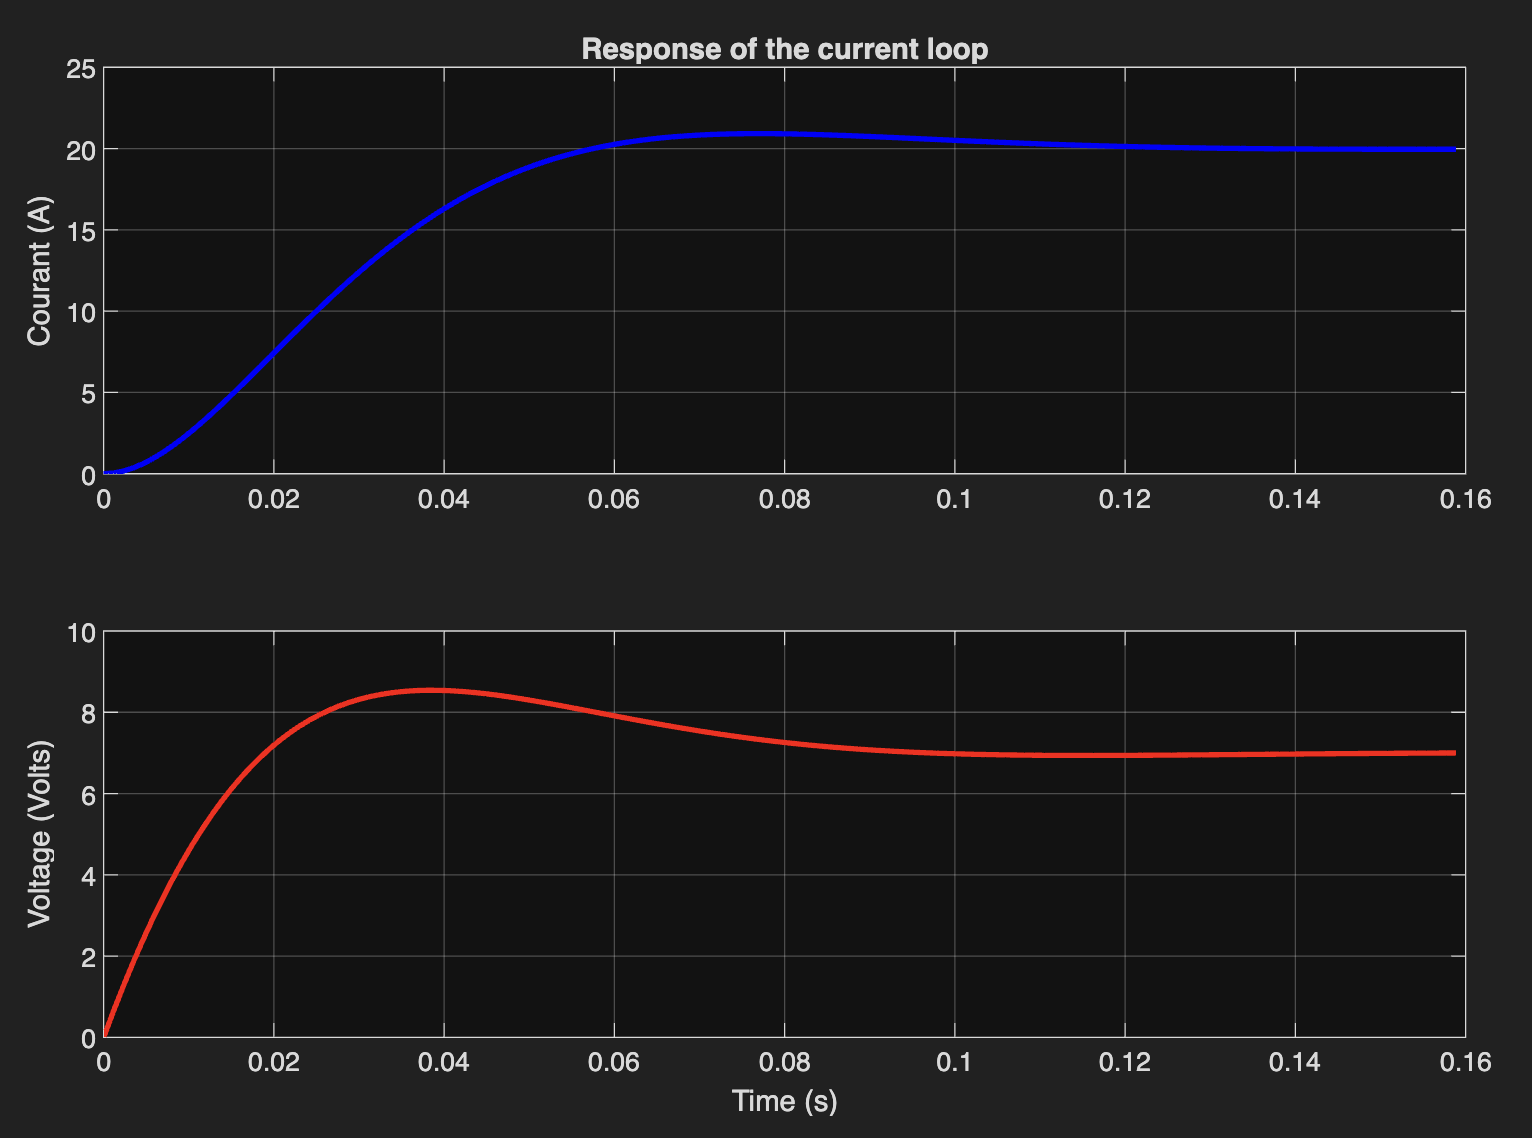
\includegraphics[width=0.85\linewidth]{figures/response_to_current_loop.png}
    \caption{Step response of the current loop to a setpoint of 20~A.}
    \label{fig:current_response}
\end{figure}

\noindent\textbf{Analysis of the results:}

The step response of the current loop shows that:
\begin{itemize}
    \item The current reaches its steady-state value of 20~A in approximately \textbf{0.1~s}.
    \item The overshoot is around \textbf{10\%}, corresponding to the damping ratio $\zeta_I = 0.7$.
    \item The system exhibits a well-damped second-order behavior with no steady-state error.
\end{itemize}

The control voltage (bottom plot) shows a smooth transient reaching about \textbf{8–9~V} before settling near 6~V once the current reaches 20~A.  
This confirms that the designed state-feedback controller ensures a fast and stable current loop, satisfying the required specifications:
\[
T_s \approx 0.1~\text{s}, \quad M_p < 10\%.
\]

Hence, the performance objectives for the current loop are successfully met.

\subsubsection{Validation with the engine simulator (TPVitessePartie21.slx)}

\paragraph{Scenario A:} $C_r=0$ and $I^\star(t)$ steps from $0$ to $20$ A at $t=1$ s.

\begin{figure}[H]
\centering
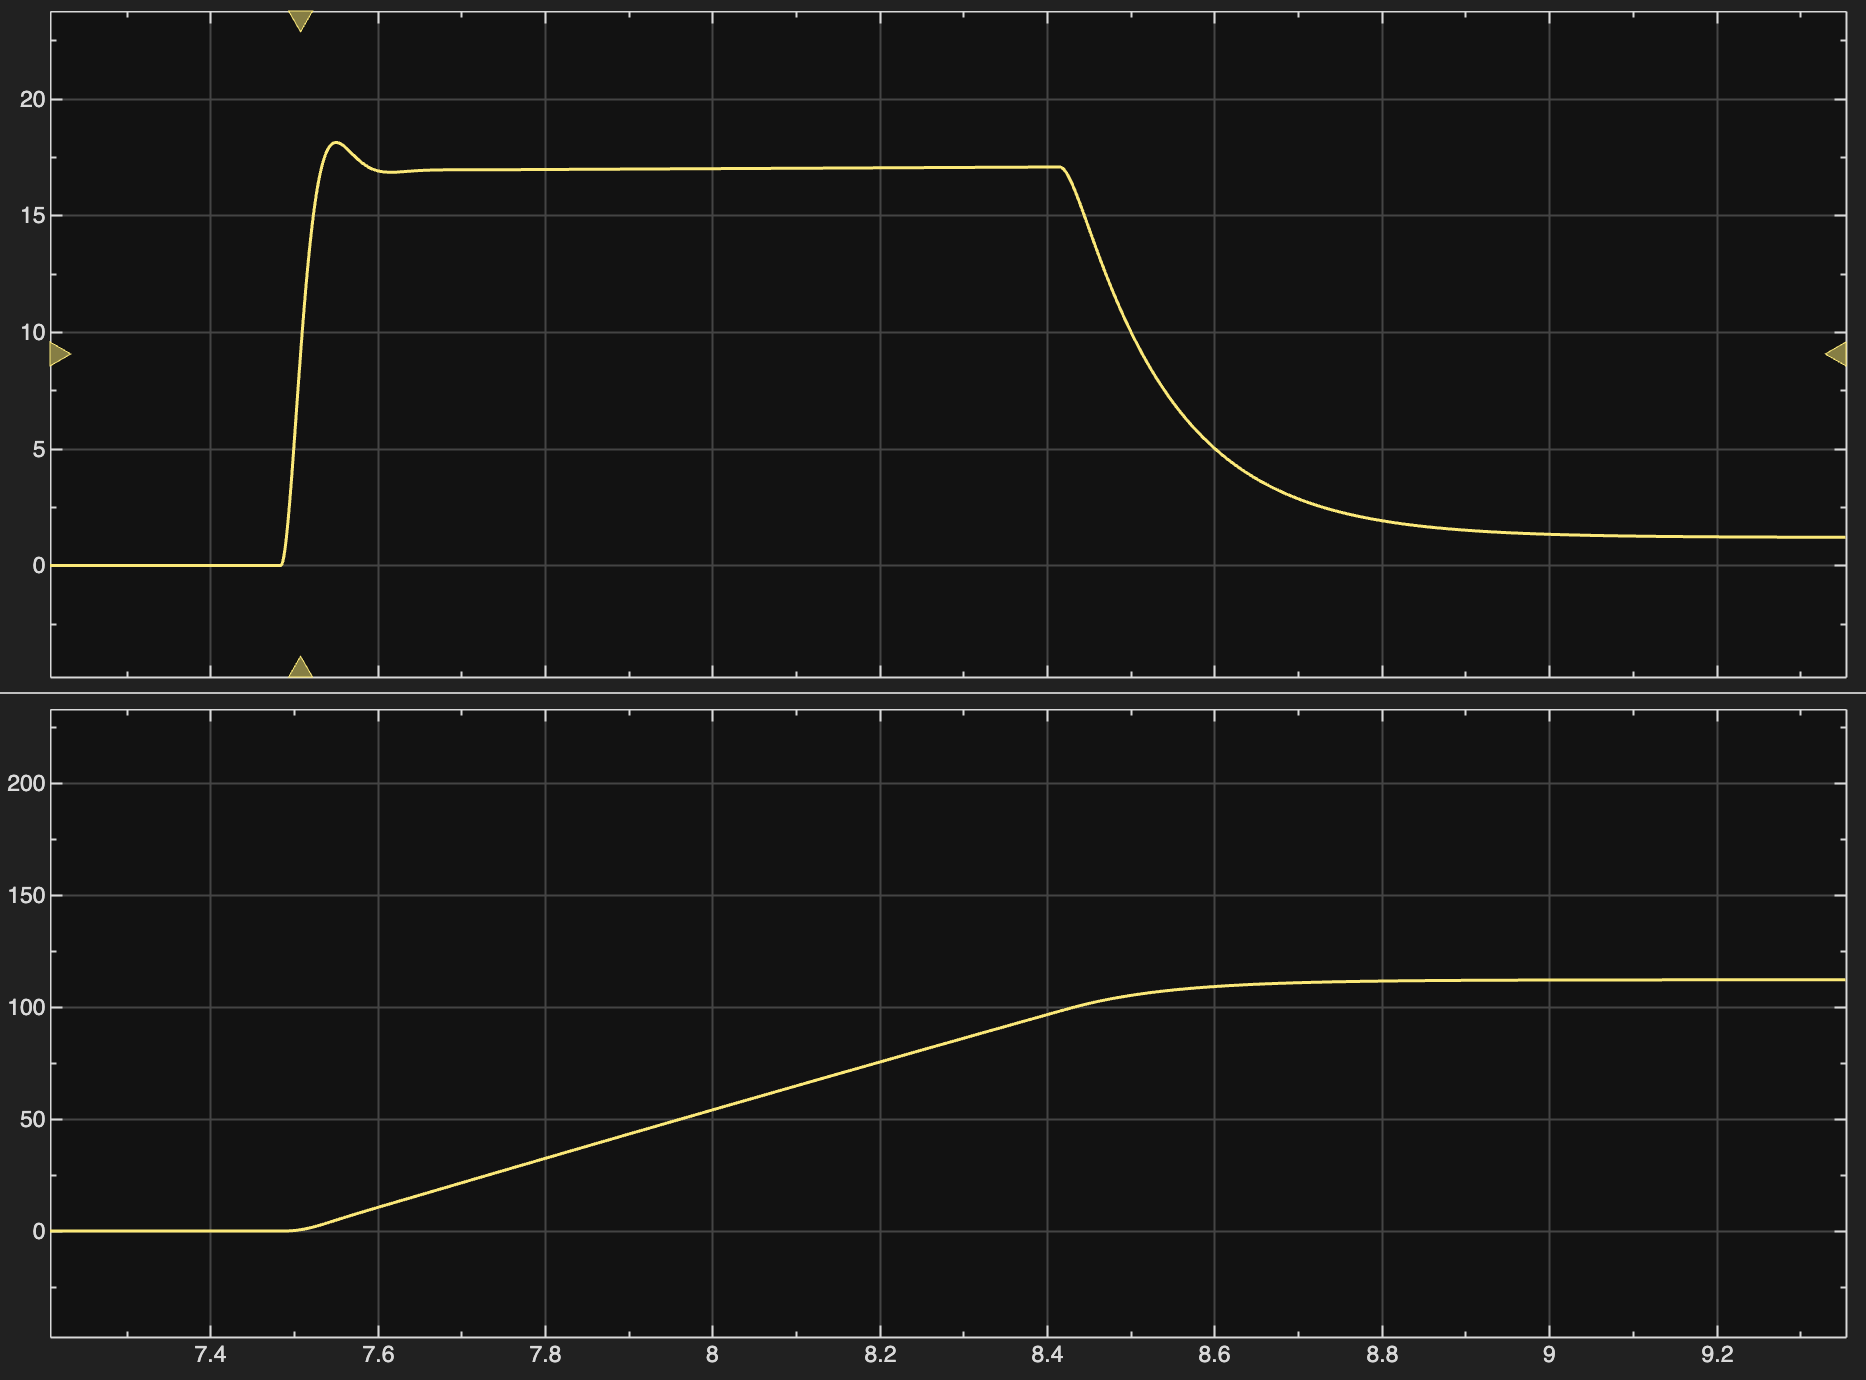
\includegraphics[width=0.95\textwidth]{figures/simulink1.png}
\caption{Scenario A — step $I^\star: 0 \rightarrow 20$ A. Top: measured current $I(t)$; bottom: speed $\Omega(t)$.}
\label{fig:part21_scnA}
\end{figure}

\textbf{Performance check.} From Fig.~\ref{fig:part21_scnA}, $I(t)$ reaches the reference with a small transient overshoot ($<10\%$), settles rapidly (order $10^{-1}$\,s), and exhibits negligible steady–state error due to the integral action in the current loop.  
\textbf{Why $I(t)$ decreases at high speed.} The electrical and mechanical dynamics are
\[
U_m = R I + L \dot I + K_e \Omega,
\qquad
J \dot \Omega = K_c I - f \Omega - C_s .
\]
As $\Omega$ grows, the back–EMF term $K_e\Omega$ increases, reducing the effective voltage available to sustain $I=20$ A. When the actuator saturates ($U_m=\pm 90$ V), the controller cannot compensate, so $I(t)$ droops slightly while $\Omega$ is high.

\paragraph{Scenario B:} $C_r=0$ and $I^\star(t)$ steps from $+10$ A to $-10$ A at $t=2$ s.

\begin{figure}[H]
\centering
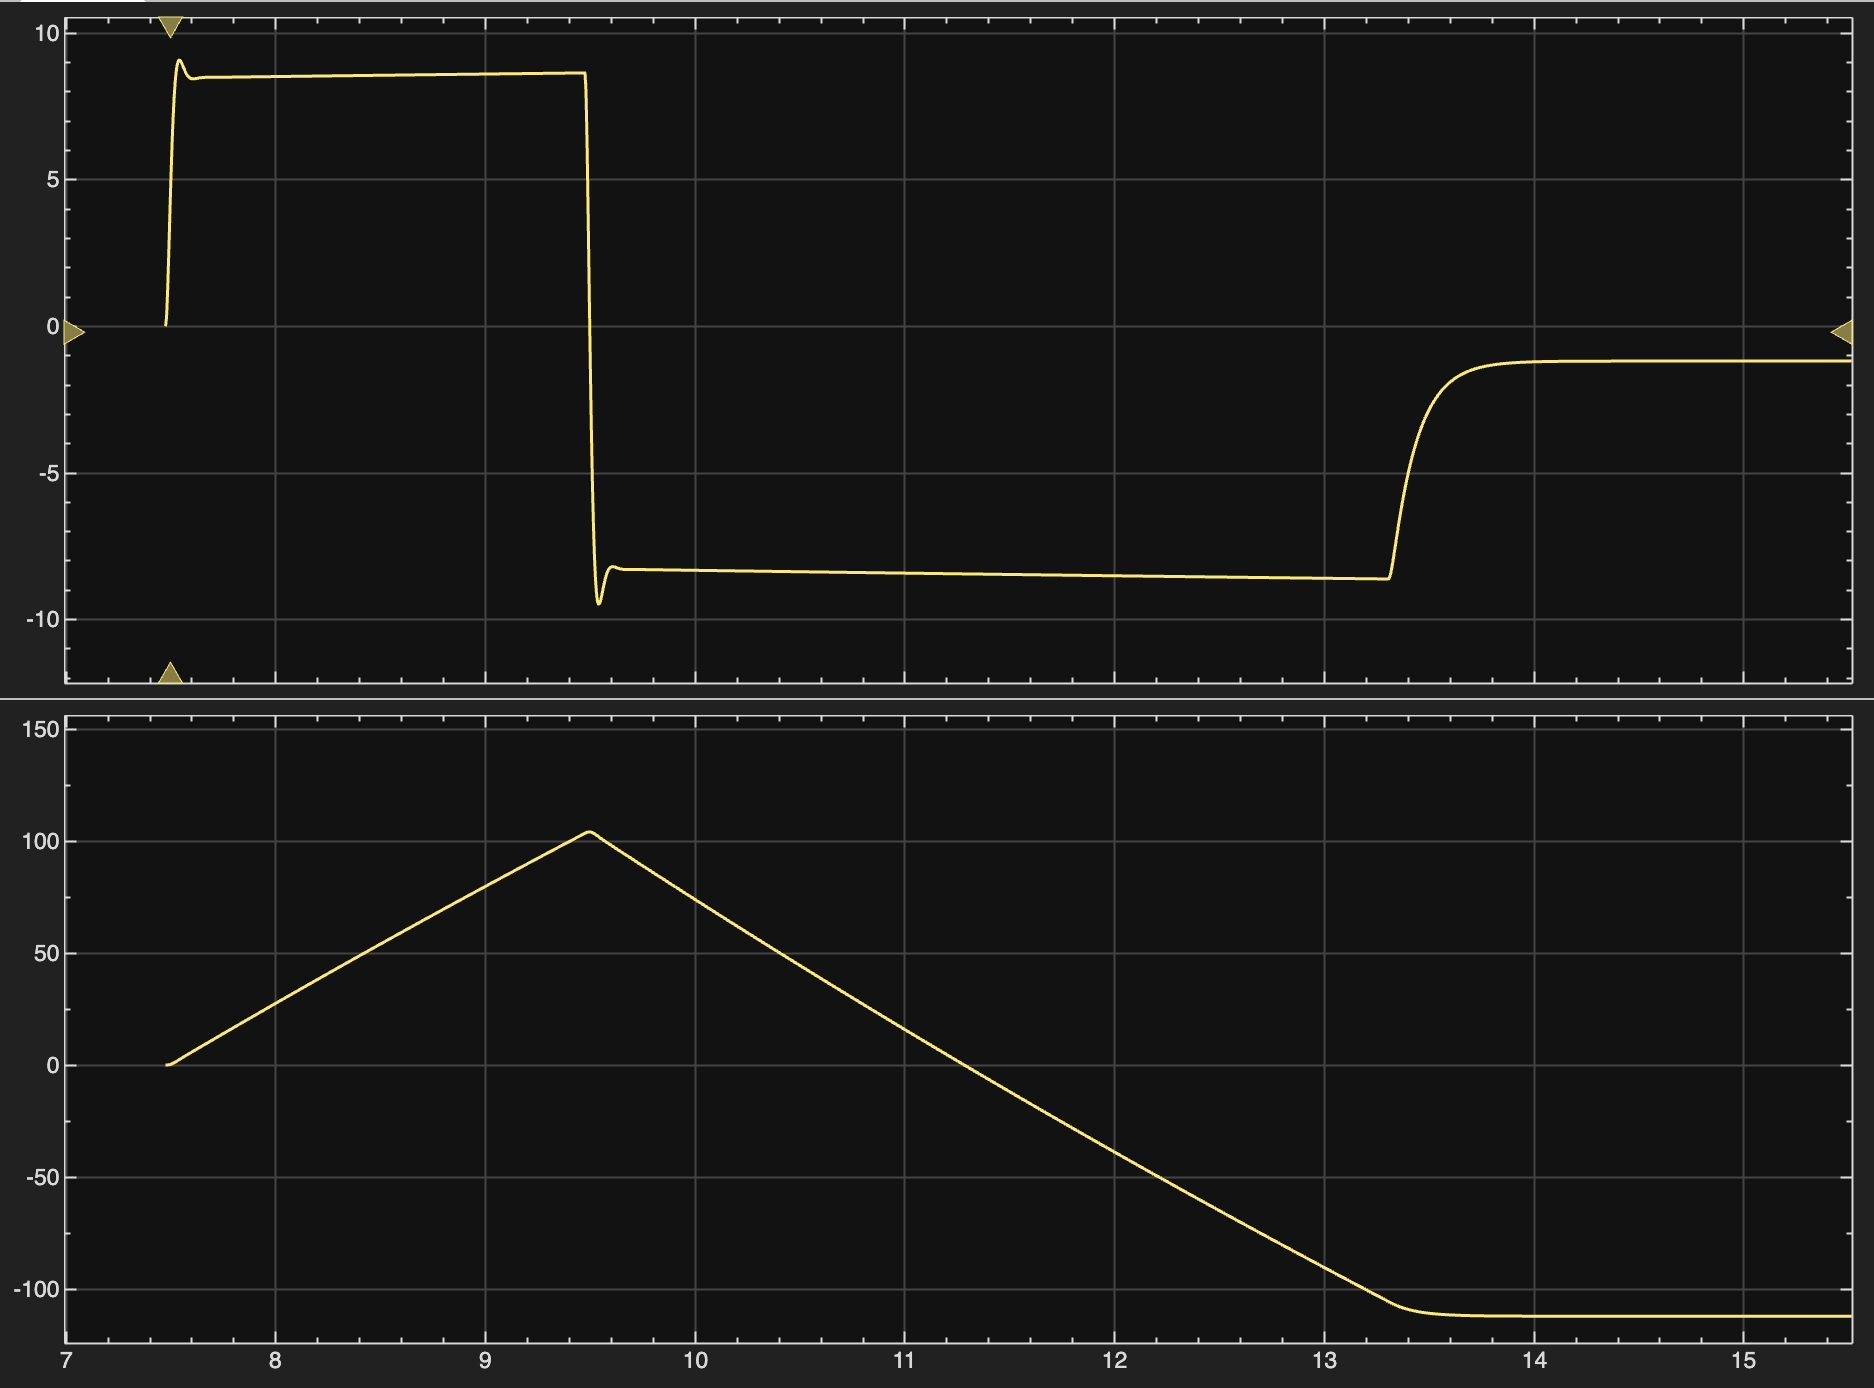
\includegraphics[width=0.95\textwidth]{figures/simulink2.png}
\caption{Scenario B — step $I^\star: +10 \rightarrow -10$ A. Top: measured current $I(t)$; bottom: $\Omega(t)$.}
\label{fig:part21_scnB}
\end{figure}

\textbf{Reason for the delay in sign reversal.} Prior to $t=2$ s, the integrator has accumulated a positive state to track $+10$ A. At the negative step, the demanded control drives $u_c$ to its limit; the integrator continues to wind up while $U_m$ is saturated, and the nonzero back–EMF $K_e\Omega$ further increases the voltage needed to reverse the current. The combination of actuator saturation and integrator windup delays the zero crossing of $I(t)$.

\textbf{Remedy.} Implement anti–windup in the current controller, e.g.\ (i) \emph{integrator clamping/conditional integration} when $u_c$ or $U_m$ saturates, or (ii) a \emph{tracking (back–calculation) loop} that drives the integrator toward the saturated actuator output. Optionally add an EMF feedforward term $U_{m,\mathrm{ff}}=K_e \Omega$ so the controller primarily regulates $R I + L \dot I$. With anti–windup, the delay is effectively removed while preserving the settling-time and overshoot specifications.

% Removed stray numbered section placeholder
\subsection{Speed Regulation by a Controller with Integrator}
\subsubsection{State-Space Model of the Augmented System}

Assuming an ideal current loop, the speed dynamics of the DC motor are given by:
\begin{equation*}
J\frac{d\Omega(t)}{dt} = K_c V_I^*(t) - C_r(t) - f\,\Omega(t)
\end{equation*}

The speed measurement is expressed as:
\begin{equation*}
V_\Omega(t) = K_{\mathrm{cap},\Omega}\,\Omega(t)
\end{equation*}

To ensure zero steady-state error and disturbance rejection, an integral of the speed error is introduced:
\begin{equation*}
x_{\varepsilon \Omega}(t) = \int_0^t \big(V_{\Omega^*}(\tau) - V_\Omega(\tau)\big)\,d\tau
\end{equation*}

The state vector and output are defined as:
\begin{equation*}
x_\Omega(t) =
\begin{bmatrix}
\Omega(t) \\[4pt]
x_{\varepsilon \Omega}(t)
\end{bmatrix},
\qquad
y_\Omega(t) = V_\Omega(t) = K_{\mathrm{cap},\Omega}\,\Omega(t)
\end{equation*}

The augmented state-space model becomes:
\begin{equation*}
\frac{d}{dt}
\begin{bmatrix}
\Omega \\[4pt]
x_{\varepsilon \Omega}
\end{bmatrix}
=
\underbrace{
\begin{bmatrix}
-\dfrac{f}{J} & 0 \\[6pt]
- K_{\mathrm{cap},\Omega} & 0
\end{bmatrix}}_{A_\Omega}
\begin{bmatrix}
\Omega \\[4pt]
x_{\varepsilon \Omega}
\end{bmatrix}
+
\underbrace{
\begin{bmatrix}
\dfrac{K_c}{J} \\[4pt]
0
\end{bmatrix}}_{B_\Omega}
V_I^*(t)
+
\underbrace{
\begin{bmatrix}
0 \\[4pt]
1
\end{bmatrix}}_{B'_\Omega}
V_{\Omega^*}(t)
+
\underbrace{
\begin{bmatrix}
-\dfrac{1}{J} \\[4pt]
0
\end{bmatrix}}_{B''_\Omega}
C_r(t)
\end{equation*}

and
\begin{equation*}
y_\Omega(t) =
\underbrace{
\begin{bmatrix}
K_{\mathrm{cap},\Omega} & 0
\end{bmatrix}}_{C_\Omega}
x_\Omega(t)
\end{equation*}

\noindent\textbf{Controllability:}
\[
\mathcal{C}_\Omega = [B_\Omega \;\; A_\Omega B_\Omega]
=
\begin{bmatrix}
\dfrac{K_c}{J} & -\dfrac{f K_c}{J^2} \\[6pt]
0 & -\dfrac{K_{\mathrm{cap},\Omega} K_c}{J}
\end{bmatrix}
\]
with
\[
\det(\mathcal{C}_\Omega) = -\frac{K_{\mathrm{cap},\Omega} K_c^2}{J^2} \neq 0
\]
Therefore, the augmented system is \textbf{controllable}.

\subsubsection{LQ Control Design}

The control law is defined as:
\begin{equation*}
V_I^*(t) = -K_\Omega\,x_\Omega(t)
= -[K_{\Omega1}\; K_{\Omega2}]
\begin{bmatrix}
\Omega(t) \\[4pt] x_{\varepsilon\Omega}(t)
\end{bmatrix}
\end{equation*}

The feedback gain $K_\Omega$ is obtained using the Linear Quadratic (LQ) approach, which minimizes the cost function:
\begin{equation*}
J(t) = \int_0^\infty \big(x_\Omega^T Q x_\Omega + r \,(V_I^*(t))^2\big)\,dt
\end{equation*}
where $Q = \mathrm{diag}(q_1, q_2)$ and $r$ are the weighting factors.

A stabilizing solution exists if $(A_\Omega,B_\Omega)$ is controllable (verified in Question~2.2.a) and if
$Q$ is positive semi-definite and $r>0$.

\noindent\textbf{Normalization of the state variables:}
\begin{itemize}
    \item $\Omega_{\max} = 1500~\mathrm{rpm} = 1500 \times 2\pi / 60$
    \item $V_{W_{\max}} = \Omega_{\max} \times K_{\mathrm{cap},\Omega}$
    \item $x_{\varepsilon\Omega,\max} = 0.5\,V_{W_{\max}} \times 0.2$
    \item $U_{\max} = 4~\mathrm{V}$
\end{itemize}

These limits are used to normalize the state and control variables prior to tuning the weighting matrices.

\noindent\textbf{MATLAB implementation:}
\begin{verbatim}
%% Question 2.2.b : LQ approach

% Normalization of the state variables
omega_max = 1500*2*pi/60;          % Maximum speed (rad/s)
VW_max = omega_max*K_capW;         % Max speed sensor voltage
q_wmax = 0.5*VW_max*0.2;           % Max integral of the error
U_max = 4;                         % Max control voltage (V)

% Scaling matrices
Qn_lq = [1/omega_max 0; 0 1/q_wmax]; 
Rn_lq = 1/U_max;

% Base weighting matrices
Q_tilda_lq = [100 0; 0 200];
R_tilda_lq = 1;

% Normalized LQ matrices
Q_lq = Qn_lq * Q_tilda_lq * Qn_lq;
R_lq = Rn_lq * R_tilda_lq * Rn_lq;

% Compute LQ gain
K_W = lqr(A_W, B_W, Q_lq, R_lq);
\end{verbatim}

\noindent The function \texttt{lqr()} returns the optimal feedback gain vector
$K_\Omega = [0.417\; -69.13]$ that minimizes $J(t)$ and ensures
a stable closed-loop behavior.

\noindent\textbf{Effect of weighting factors:}
\begin{itemize}
    \item Increasing $q_1$ emphasizes faster speed tracking but may cause larger control efforts.
    \item Increasing $q_2$ improves disturbance rejection (faster integral action).
    \item Increasing $r$ reduces the control voltage amplitude but slows down the response.
\end{itemize}

A suitable balance between $Q$ and $r$ results in a settling time close to
$2~\mathrm{s}$ and an overshoot below $10\%$, as required by the design specifications.


\subsubsection{Validation of the speed controller}

The objective of this part is to evaluate the performance of the speed control loop implemented in \textsc{Matlab/Simulink} under different operating conditions.  
The control law is tested with various speed setpoints $\Omega^\star(t)$ and with/without a load torque $C_r(t)$.

\paragraph{Scenario 1:} $C_r(t)=0$, the setpoint $\Omega^\star(t)$ changes from $0$ to $300$~rpm at $t=1$~s.
\begin{figure}[H]
\centering
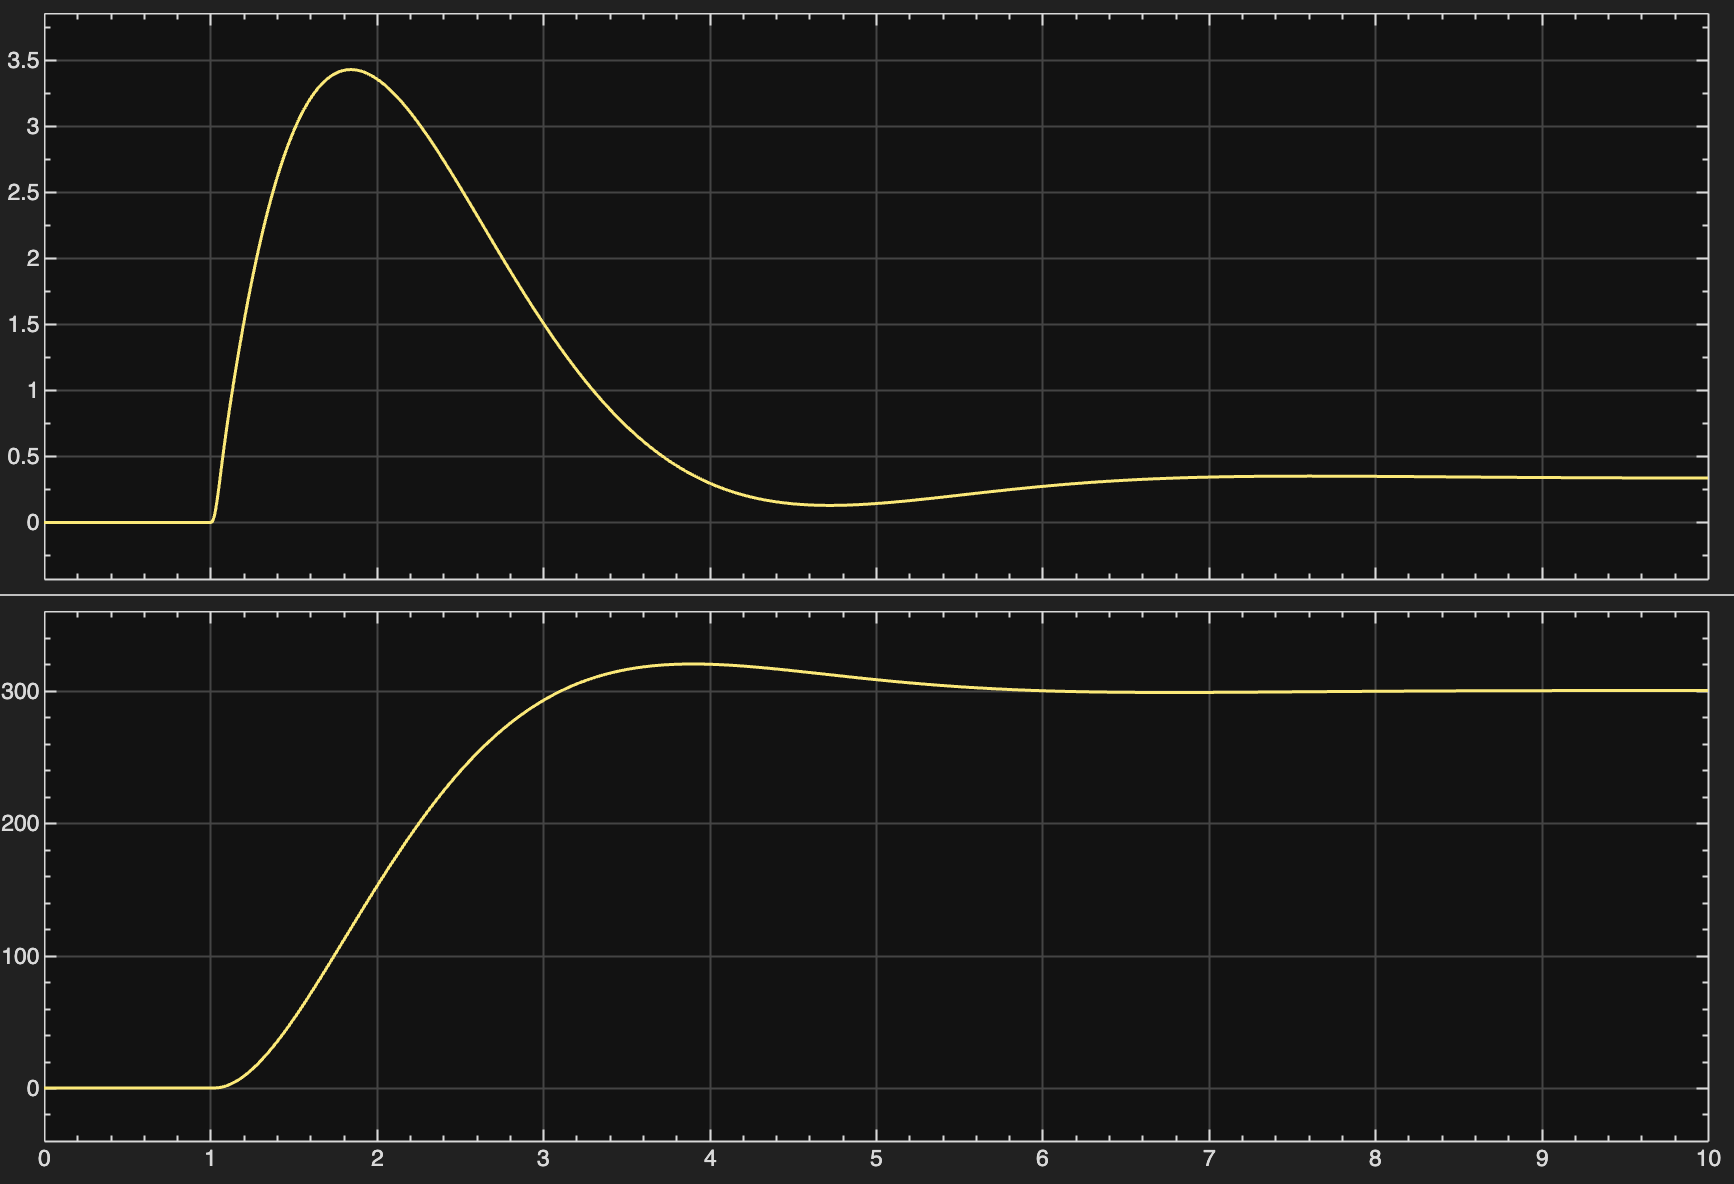
\includegraphics[width=0.9\textwidth]{figures/simulink3.png}
\caption{Scenario 1 — $\Omega^\star(t)$ step from $0$ to $300$~rpm at $t=1$~s.}
\label{fig:simulink3}
\end{figure}

\paragraph{Scenario 2:} $C_r(t)=0$, the setpoint $\Omega^\star(t)$ changes from $0$ to $500$~rpm at $t=1$~s.
\begin{figure}[H]
\centering
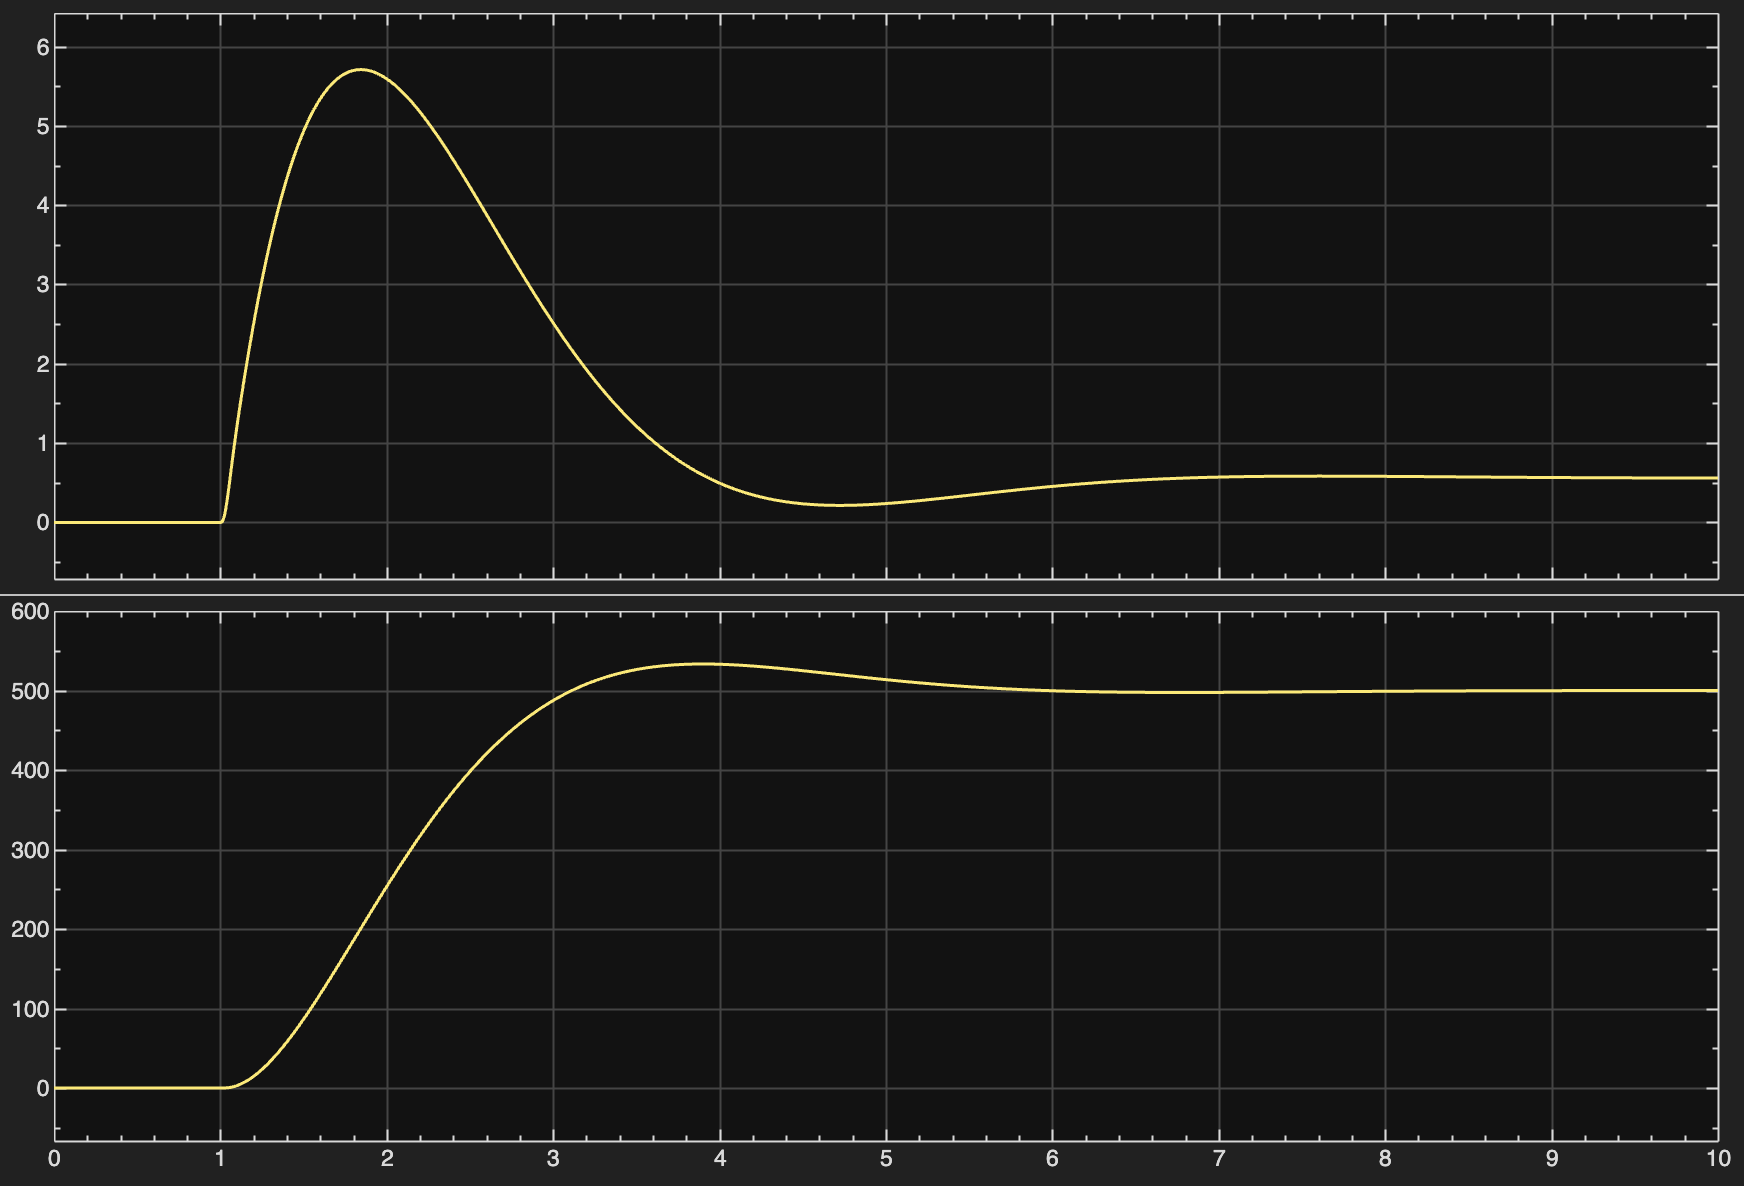
\includegraphics[width=0.9\textwidth]{figures/simulink4.png}
\caption{Scenario 2 — $\Omega^\star(t)$ step from $0$ to $500$~rpm at $t=1$~s.}
\label{fig:simulink4}
\end{figure}

\paragraph{Scenario 3:} $C_r(t)=0$, the setpoint $\Omega^\star(t)$ changes from $0$ to $1200$~rpm at $t=1$~s.
\begin{figure}[H]
\centering
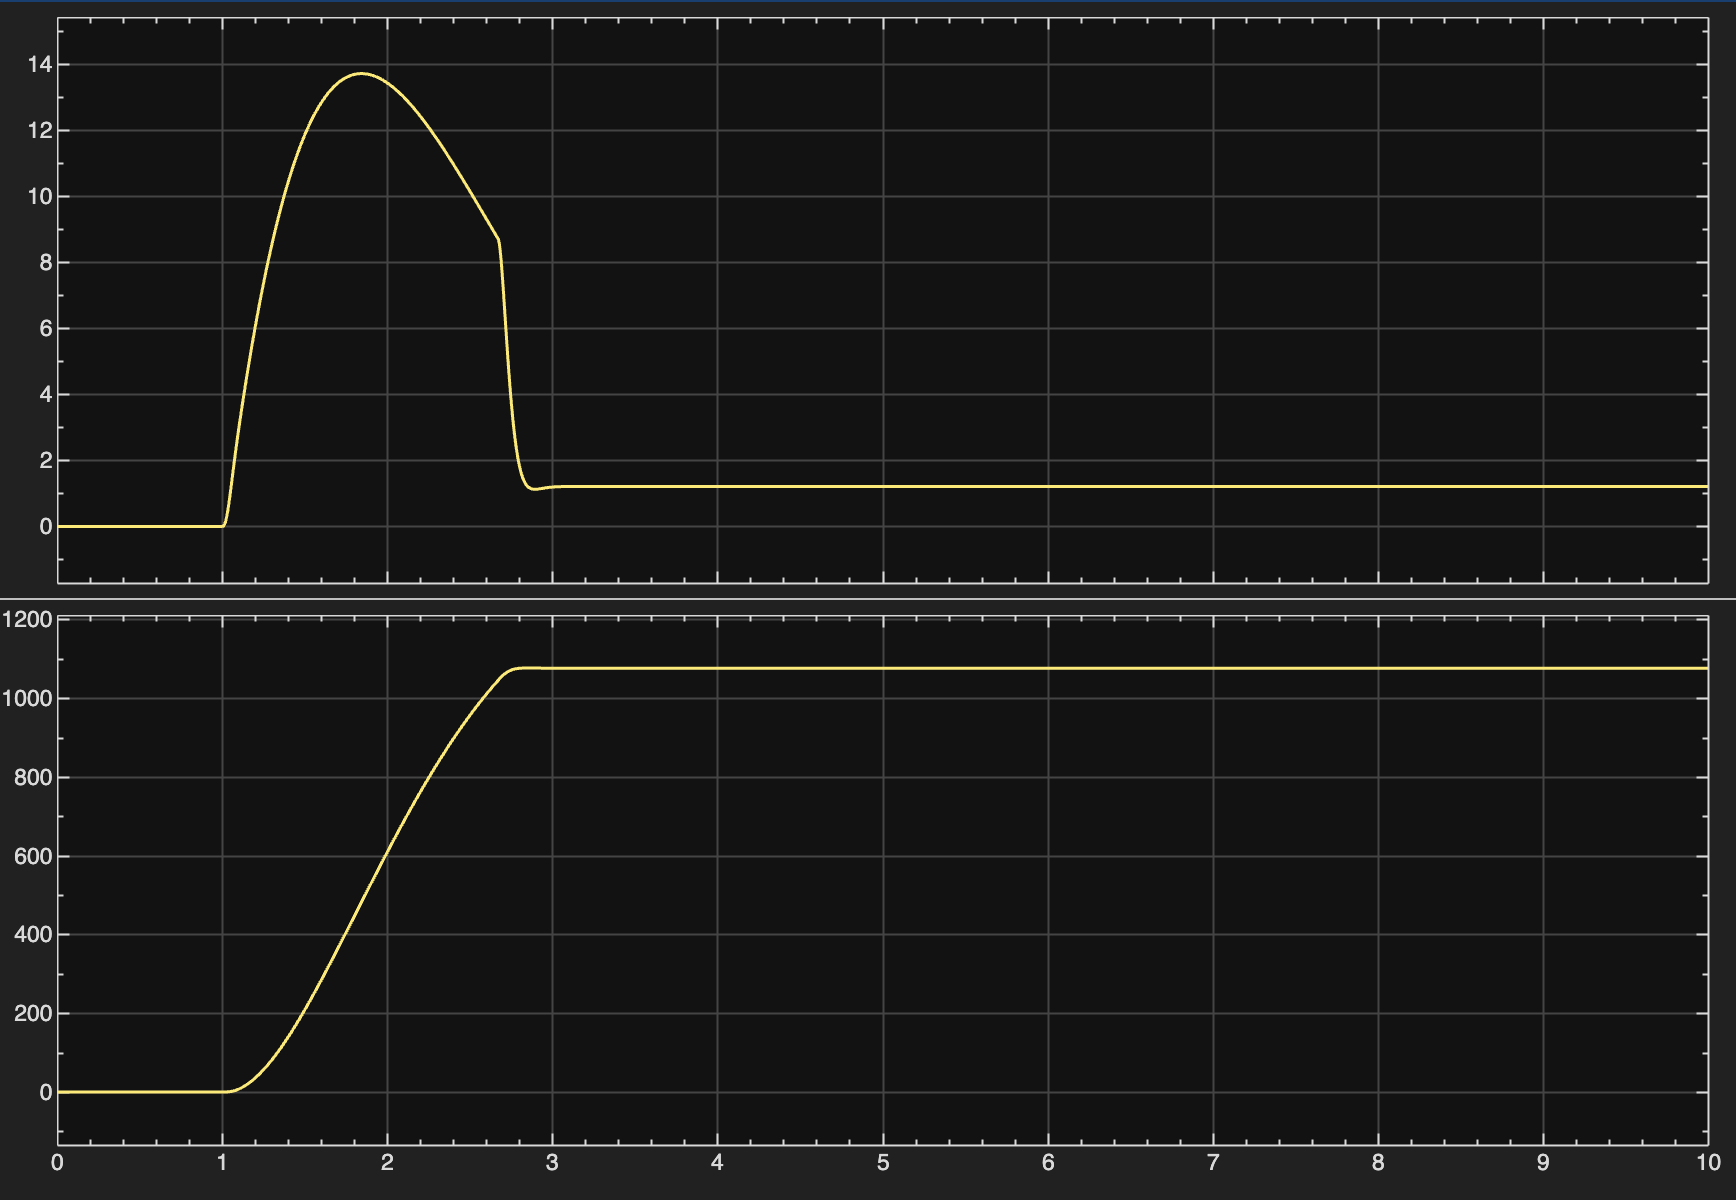
\includegraphics[width=0.9\textwidth]{figures/simulink5.png}
\caption{Scenario 3 — $\Omega^\star(t)$ step from $0$ to $1200$~rpm at $t=1$~s.}
\label{fig:simulink5}
\end{figure}

\paragraph{Scenario 4:} The load torque $C_r(t)$ changes from $0$ to $5$~N·m at $t=10$~s, while the setpoint $\Omega^\star(t)$ changes from $0$ to $300$~rpm at $t=1$~s.
\begin{figure}[H]
\centering
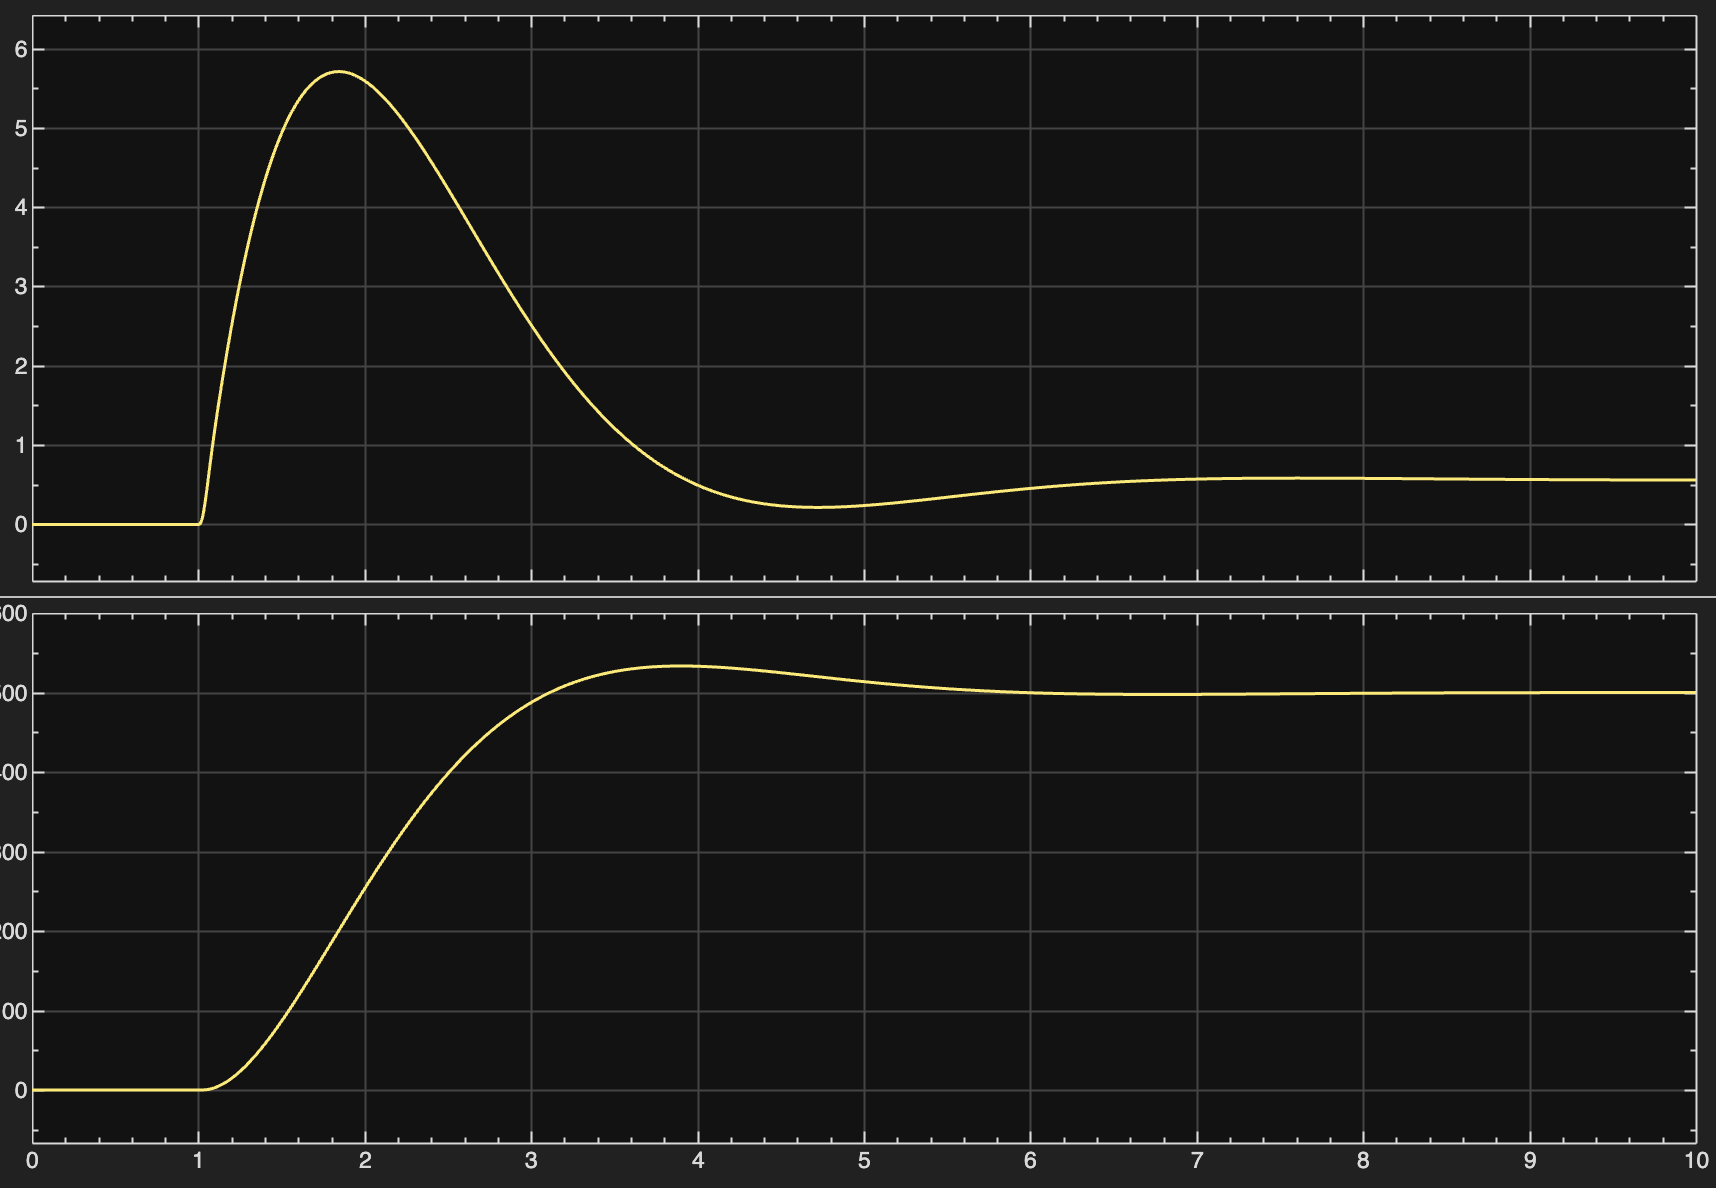
\includegraphics[width=0.9\textwidth]{figures/simulink6.png}
\caption{Scenario 4 — $\Omega^\star(t)$ step from $0$ to $300$~rpm at $t=1$~s with $C_r(t)$ disturbance at $t=10$~s.}
\label{fig:simulink6}
\end{figure}

\paragraph{Analysis.}
Each test allows evaluation of the system’s dynamic behavior in terms of rise time, overshoot, and steady–state accuracy.  
Scenarios~1–3 demonstrate the controller’s response to increasing speed references, highlighting its bandwidth and saturation limits.  
Scenario~4 evaluates the robustness of the controller to load disturbances, verifying that the integral component ensures steady–state compensation of $C_r$ while maintaining the desired speed.

\subsubsection{Stability Margin Analysis}

The stability of the designed LQ speed controller can be analyzed by examining the open-loop transfer function of the system defined by:
\begin{equation*}
\dot{x}_\Omega(t) = A_\Omega x_\Omega(t) + B_\Omega u(t),
\qquad
y(t) = K_\Omega x_\Omega(t)
\end{equation*}

The open-loop system is implemented in MATLAB and converted to a transfer function form to determine the gain and phase margins using the \texttt{margin()} function.

\noindent\textbf{MATLAB implementation:}
\begin{verbatim}
% Question 2.2.d : Stability margin analysis

C_bo = K_W;              % Controller acts as output matrix
D_bo = 0;                % No direct transmission term
sys_bo = ss(A_W, B_W, C_bo, D_bo);  % Open-loop state-space model
G_bo = tf(sys_bo);       % Convert to transfer function

figure(3)
margin(G_bo);            % Bode plot with margins
grid on

[GM, PM, Wcg, Wcp] = margin(G_bo);
fprintf('\n--- Stability margins ---\n');
fprintf('Gain margin = %.2f dB\n', 20*log10(GM));
fprintf('Phase margin = %.2f°\n', PM);
fprintf('Gain crossover frequency = %.2f rad/s\n', Wcg);
fprintf('Phase crossover frequency = %.2f rad/s\n', Wcp);
\end{verbatim}

\noindent\textbf{Obtained results:}
\begin{itemize}
    \item Gain margin: $\infty~\mathrm{dB}$
    \item Phase margin: $73.31^{\circ}$
    \item Gain crossover frequency: not defined (system always stable)
    \item Phase crossover frequency: $28.54~\mathrm{rad/s}$
\end{itemize}

\begin{figure}[H]
    \centering
    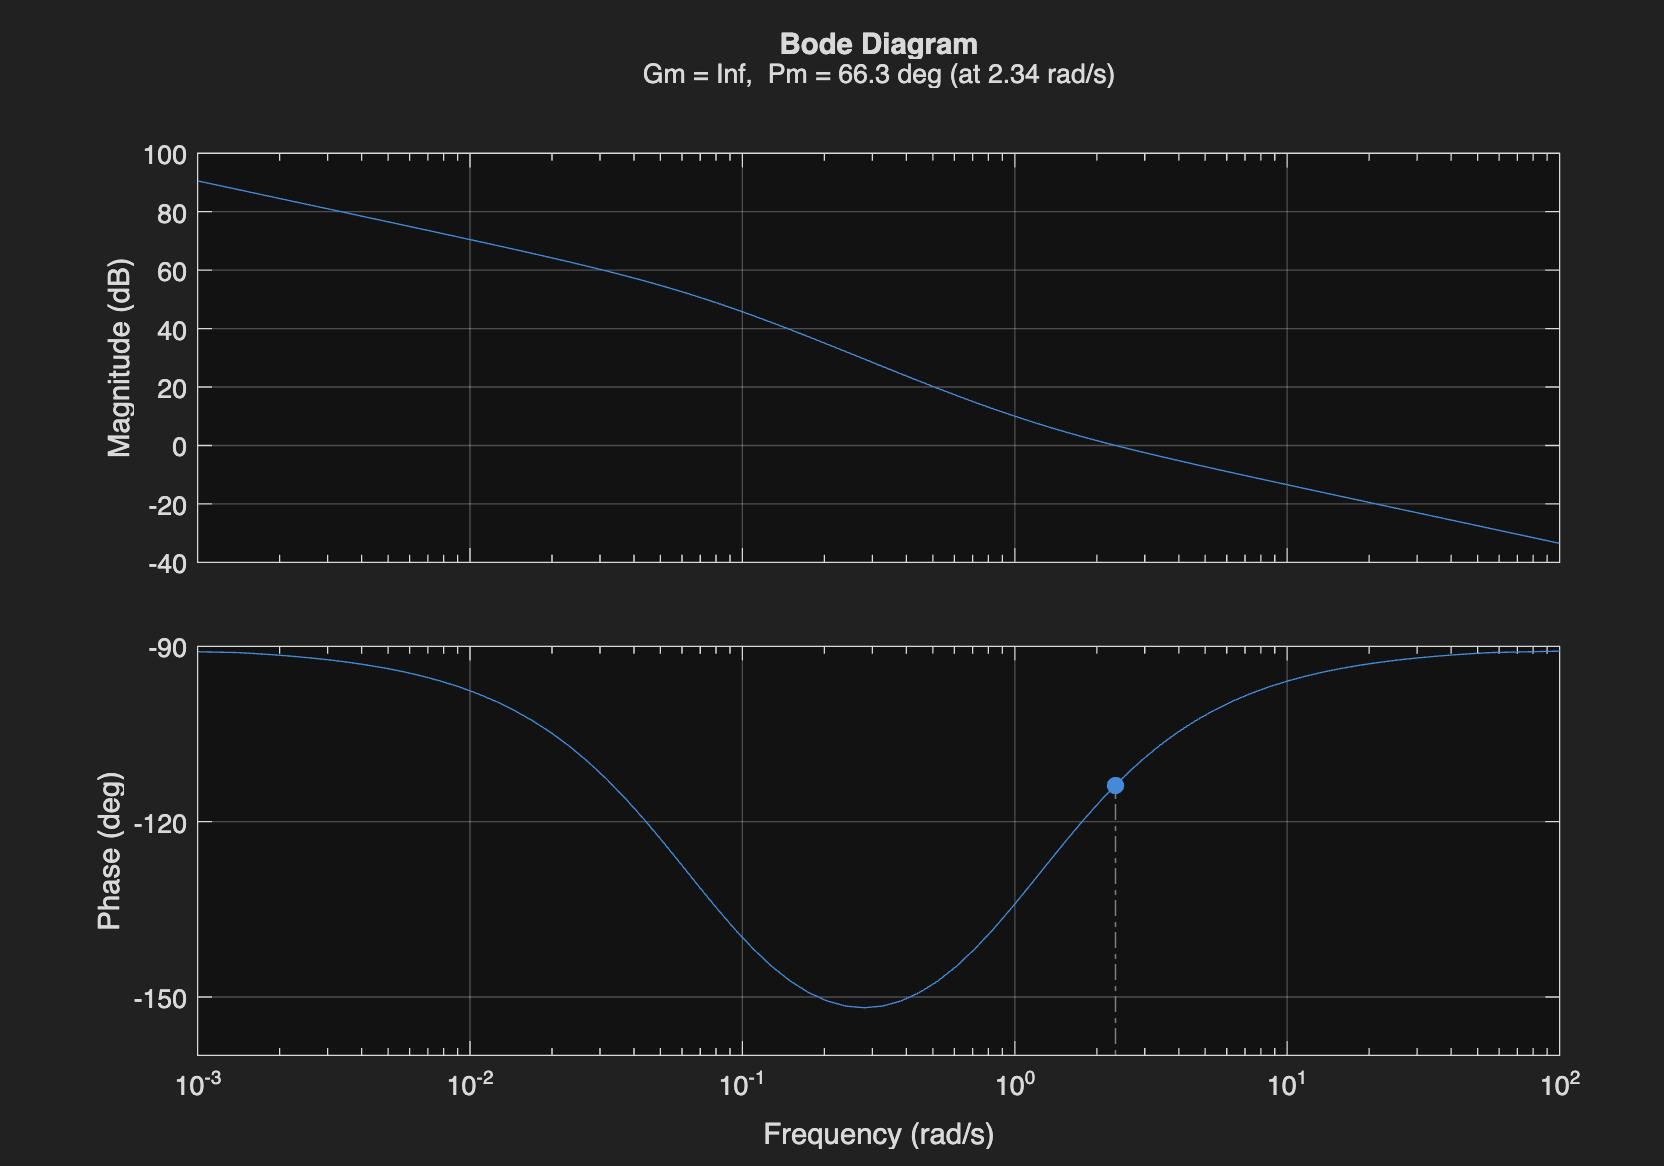
\includegraphics[width=0.85\linewidth]{figures/bode.png}
    \caption{Bode diagram of the open-loop speed control system.}
    \label{fig:bode_speed_loop}
\end{figure}

\noindent\textbf{Interpretation of results:}
\begin{itemize}
    \item The infinite gain margin indicates that the system remains stable for all practical gain variations — the open-loop gain does not cross 0~dB.
    \item The phase margin of $73.3^{\circ}$ demonstrates a high robustness and well-damped transient response.
    \item The crossover frequency of $28.5~\mathrm{rad/s}$ defines the approximate bandwidth of the speed loop, ensuring sufficient speed-tracking capability without excessive oscillations.
\end{itemize}

In conclusion, the LQ-designed controller provides a highly stable and robust speed control system, satisfying the required performance criteria for both stability and dynamic behavior.

\subsection{Design of an Observer Capable of Reconstructing the Resistant Torque}
\subsubsection{Augmented System and Observability}

The augmented state-space model of the DC machine used for the observer design is given by:
\begin{equation*}
\frac{d x_a(t)}{dt} = A_a x_a(t) + B_a u_c(t), \qquad y_a(t) = C_a x_a(t)
\end{equation*}
where the state vector and output are:
\[
x_a = 
\begin{bmatrix}
I \\[4pt] \Omega \\[4pt] C_r
\end{bmatrix}, 
\quad
y_a = V_I
\]

The matrices of the augmented system are defined as:
\begin{equation*}
A_a = 
\begin{bmatrix}
-\dfrac{R}{L} & -\dfrac{K_c}{L} & 0 \\[6pt]
\dfrac{K_c}{J} & -\dfrac{f}{J} & -\dfrac{1}{J} \\[6pt]
0 & 0 & 0
\end{bmatrix},
\quad
B_a =
\begin{bmatrix}
\dfrac{k_h}{L} \\[4pt] 0 \\[4pt] 0
\end{bmatrix},
\quad
C_a = 
\begin{bmatrix}
K_{\mathrm{cap}I} & 0 & 0
\end{bmatrix},
\quad
D_a = \mathbf{0}_{3\times1}
\end{equation*}

\noindent\textbf{MATLAB implementation:}
\begin{verbatim}
A_a = [-R/L  -Kc/L  0;
        Kc/J  -f/J  -1/J;
        0      0     0];
B_a = [kh/L; 0; 0];
C_a = [K_capI 0 0];
D_a = zeros(3,1);

QO_a = obsv(A_a, C_a);   % Observability matrix
rank(QO_a)               % Check the observability rank
\end{verbatim}

\noindent The observability matrix has full rank $(\mathrm{rank}(QO_a)=3)$, confirming that the system is \textbf{observable}.

\subsubsection{Selection of Observer Dynamics}

According to the design requirements, the observer must be approximately three times faster than the speed control loop.  
The damping ratio and crossover frequency are set as:
\[
\zeta_{\mathrm{n}\Omega} = 0.7, \qquad \omega_{\mathrm{n}\Omega} = \frac{3\times4}{0.7\times0.1}
\]
The desired observer eigenvalues are then computed from the characteristic polynomial:
\[
\lambda^2 + 2\zeta_{\mathrm{n}\Omega}\omega_{\mathrm{n}\Omega}\lambda + \omega_{\mathrm{n}\Omega}^2 = 0
\]
and an additional third eigenvalue is added, chosen to be twice as fast as the previous ones.

\noindent\textbf{MATLAB implementation:}
\begin{verbatim}
zeta_nW = 0.7;                           % Damping coefficient
omega_nW = 3*4/(0.7*0.1);                % Crossover frequency
lambda_W = roots([1, 2*zeta_nW*omega_nW, omega_nW^2]);
lambda_W = [lambda_W; sum(lambda_W)];    % Add a faster 3rd pole
lambda_obs = lambda_W;                   % Observer eigenvalues
\end{verbatim}

\noindent These eigenvalues ensure that the observer converges rapidly to the actual system states while maintaining numerical stability.

\subsubsection{Observer design from current measurement and control input}

We reconstruct the augmented state
\[
x_a=\begin{bmatrix} I & \Omega & C_r \end{bmatrix}^\top,
\qquad y_a = V_I = K_{\mathrm{cap}I}\,I,
\]
using a Luenberger observer driven by the measured current \(y_a\) and the control \(u_c\).
With the augmented plant
\[
\dot x_a = A_a x_a + B_a u_c, \qquad y_a = C_a x_a ,
\]
the observer is chosen as
\[
\boxed{\;
\dot{\hat x}_a = (A_a - K_{\mathrm{obs}} C_a)\,\hat x_a + B_a u_c + K_{\mathrm{obs}}\,y_a,
\qquad
y_{\mathrm{obs}} = C_{\mathrm{obs}}\,\hat x_a,
\;}
\]
where \(y_{\mathrm{obs}}=\begin{bmatrix}\hat I & \hat\Omega & \hat C_r\end{bmatrix}^\top\) and typically
\(C_{\mathrm{obs}}=I_3\).
The gain \(K_{\mathrm{obs}}\) is computed by pole placement to make the observer dynamics
significantly faster than the plant (e.g., \(3\!-\!5\times\) the closed-loop bandwidth).

Equivalently, grouping \(u_c\) and \(y_a\) as inputs,
\[
\dot{\hat x}_a = A_{\mathrm{obs}}\hat x_a + B_{\mathrm{obs}}
\begin{bmatrix} u_c \\ y_a \end{bmatrix},
\quad
A_{\mathrm{obs}} = A_a - K_{\mathrm{obs}} C_a,\quad
B_{\mathrm{obs}}=\begin{bmatrix} B_a & K_{\mathrm{obs}} \end{bmatrix}.
\]

\paragraph{MATLAB implementation (matching the above):}
\begin{lstlisting}[language=Matlab]
% Given: A_a, B_a, C_a, desired observer poles lambda_obs (1x3)
K_obs = place(A_a', C_a', lambda_obs')';   % Luenberger gain

A_obs = A_a - K_obs*C_a;                   % Observer A
B_obs = [B_a, K_obs];                      % Inputs [u_c; y_a]
C_obs = eye(3);                            % Outputs [Î; Ω̂; Ĉr]
D_obs = zeros(3,2);
\end{lstlisting}

\noindent
\textit{Notes.} (i) Ensure \((A_a,C_a)\) is observable. (ii) Choose \(\lambda_{\text{obs}}\) real or complex
with negative real parts and magnitude \(3\!-\!5\) times larger than the controller poles to obtain fast,
well-damped convergence of \([\hat I,\hat\Omega,\hat C_r]\) to their true values.

\subsubsection{Observer implementation and convergence check}

We implement a Luenberger observer that reconstructs the state
\[
x_c=\begin{bmatrix} I & \Omega & C_r \end{bmatrix}^\top
\]
from the measured armature current $V_I=K_{\mathrm{cap}I}\,I$ and the available control input $u_c$.
With the augmented plant
\[
\dot x_c = A_c\,x_c + B_c\,u_c, \qquad y_c = C_c\,x_c \;\; (y_c=V_I),
\]
the observer is
\[
\dot{\hat x}_c = A_c\,\hat x_c + B_c\,u_c + K_{\mathrm{obs}}\,(y_c-\hat y_c),
\qquad \hat y_c = C_c\,\hat x_c,
\]
where $K_{\mathrm{obs}}$ is chosen so that the observer poles are about three times faster than the
current-loop poles (as required), ensuring rapid convergence.

\paragraph{Convergence results.}
Figures~\ref{fig:obs_I}–\ref{fig:obs_Cr} compare the estimated variables
$\big[\hat I,\;\hat\Omega,\;\hat C_r\big]$ with their true values obtained from the simulator.

\begin{figure}[H]
\centering
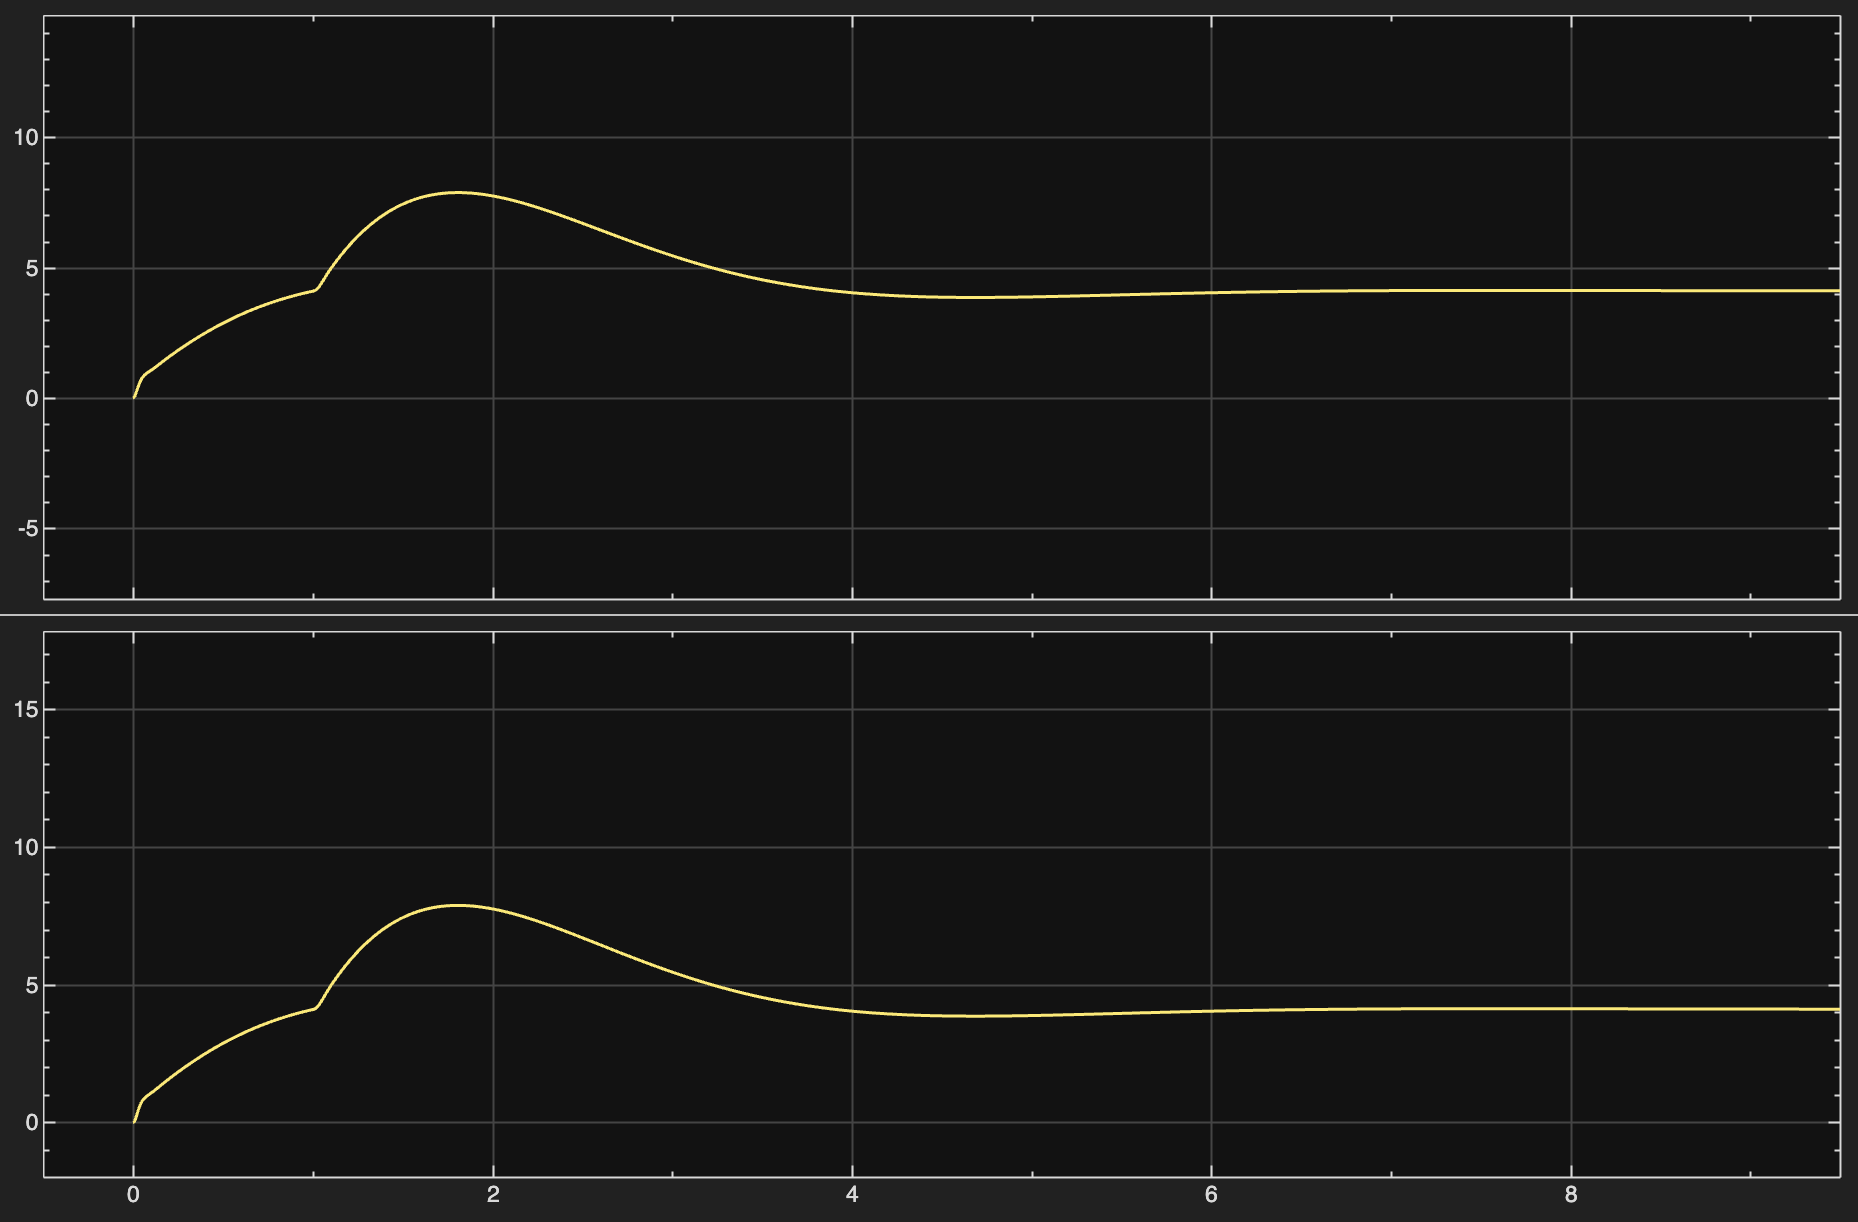
\includegraphics[width=0.95\textwidth]{figures/simulinkcurrent.png}
\caption{Current estimation: measured/true $I(t)$ vs.\ $\hat I(t)$. The estimate rapidly converges after a short transient.}
\label{fig:obs_I}
\end{figure}

\begin{figure}[H]
\centering
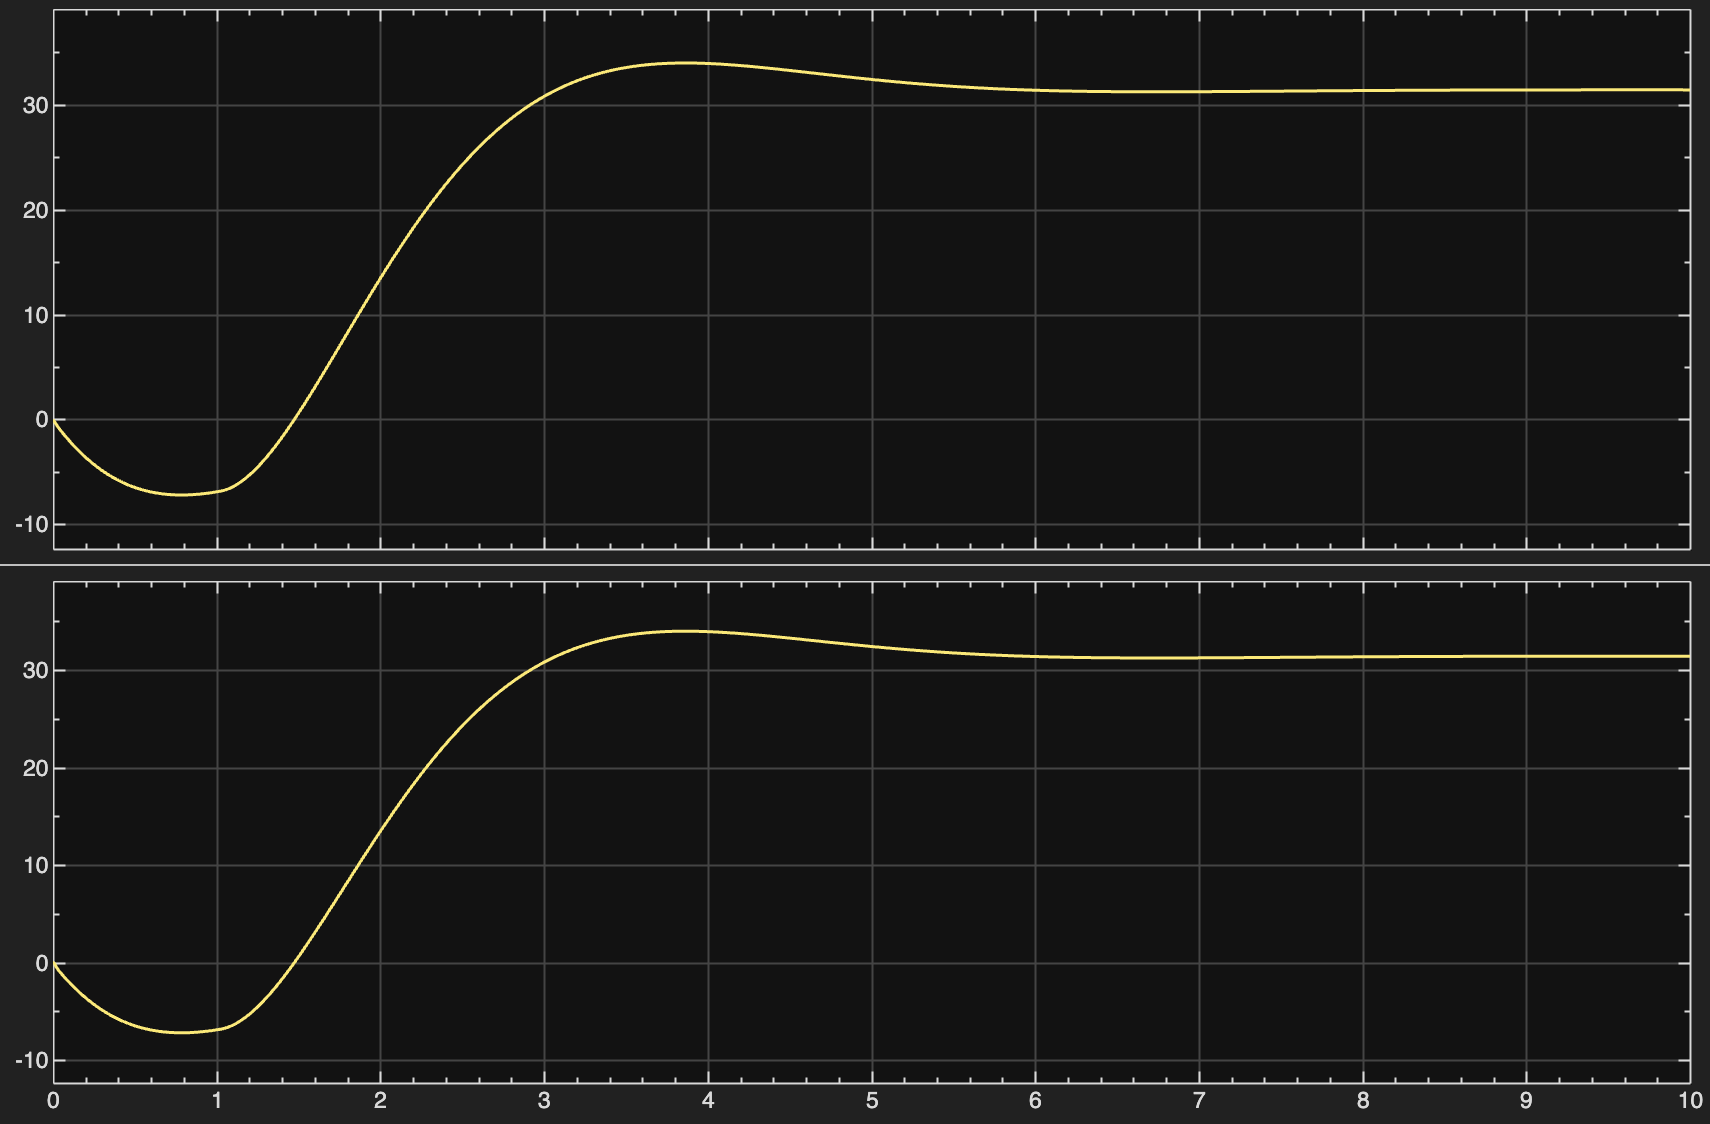
\includegraphics[width=0.95\textwidth]{figures/simulinkspeed.png}
\caption{Speed estimation: true $\Omega(t)$ vs.\ $\hat\Omega(t)$. The reconstruction tracks the reference dynamics with small transient error.}
\label{fig:obs_Omega}
\end{figure}

\begin{figure}[H]
\centering
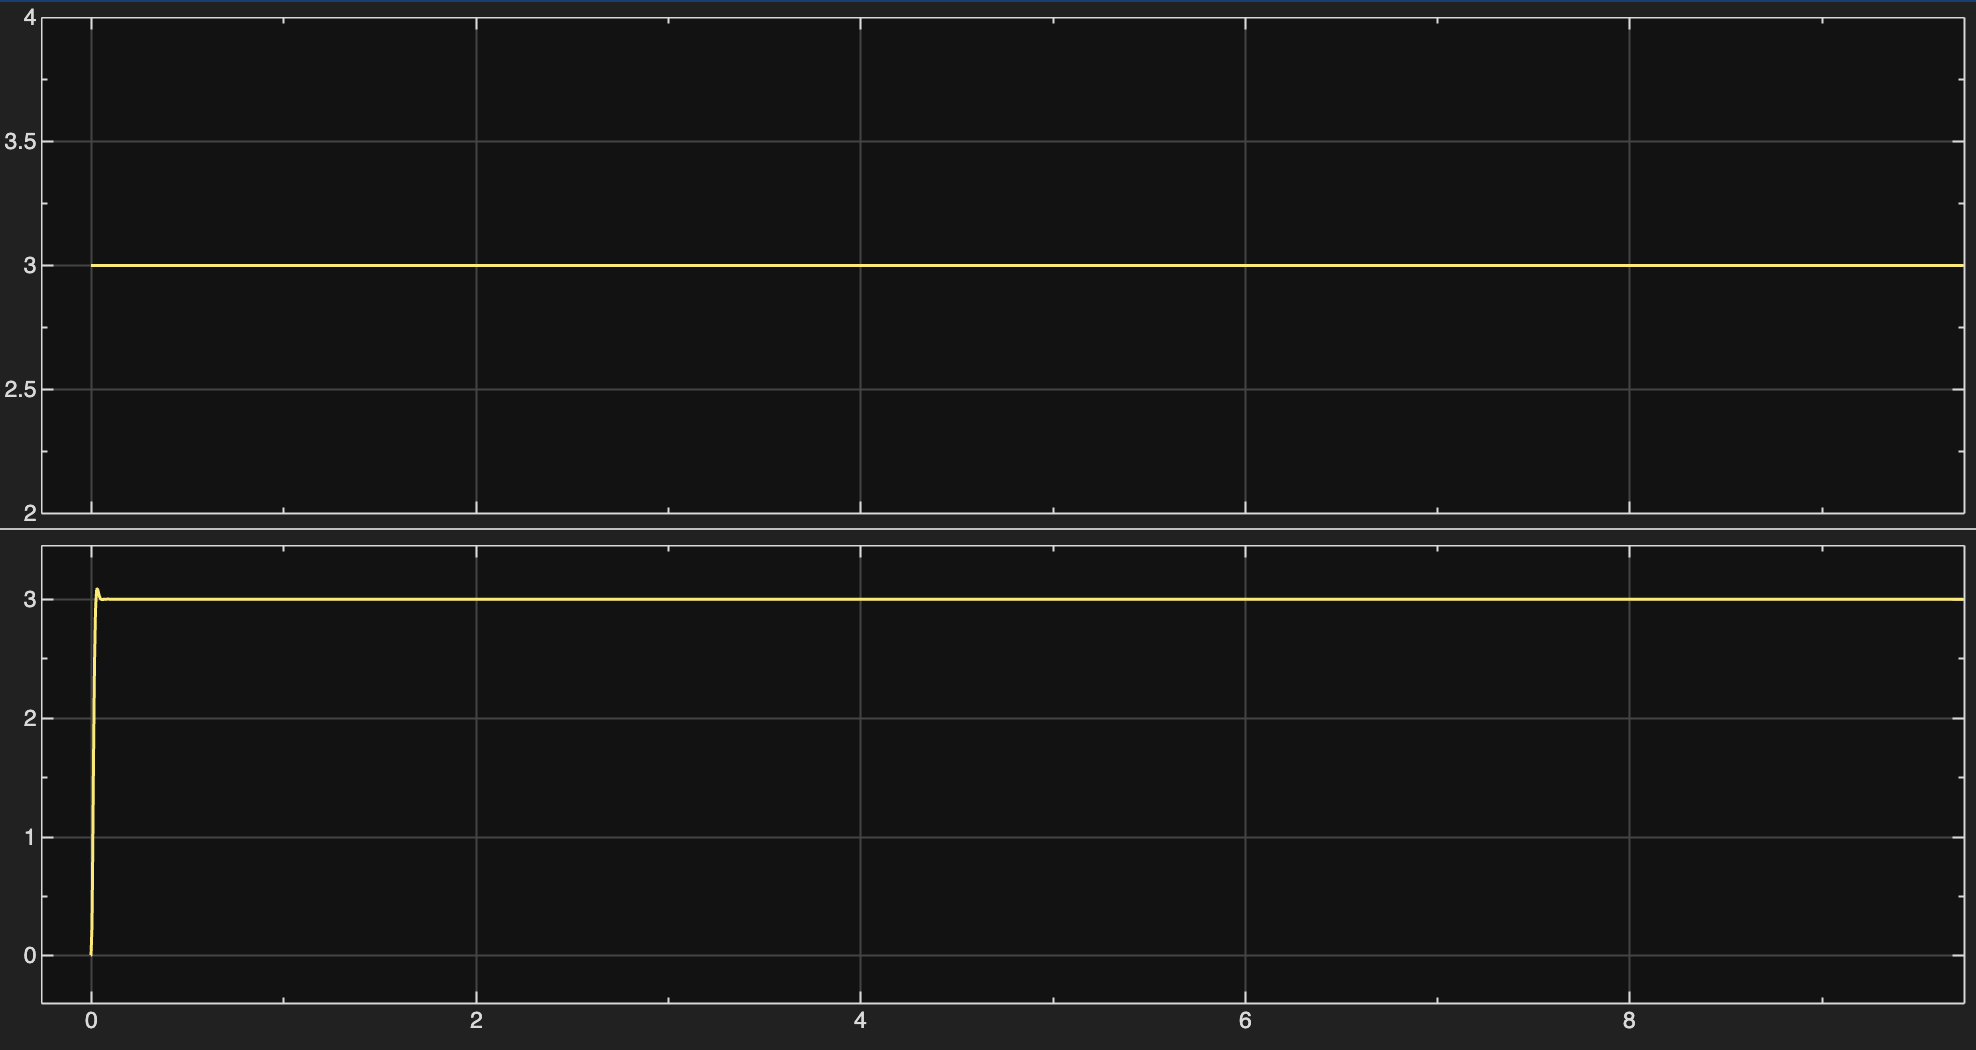
\includegraphics[width=0.95\textwidth]{figures/simulinkdisturbance.png}
\caption{Disturbance torque estimation: true $C_r(t)$ vs.\ $\hat C_r(t)$. The observer converges to the (piecewise constant) applied disturbance.}
\label{fig:obs_Cr}
\end{figure}

\paragraph{Comment.}
Across all tests the estimated variables converge quickly to their true values, with only a brief
initial transient and negligible steady-state bias, which validates the observer design and the choice of
$K_{\mathrm{obs}}$ (fast poles).

\subsubsection{Determination of the Observer Gain}

The observer gain $K_{\mathrm{obs}}$ is computed by pole placement, ensuring the desired dynamic performance.  
Using the transposed system matrices, we find:
\begin{equation*}
K_{\mathrm{obs}} = \texttt{place}(A_a', C_a', \lambda_{\mathrm{obs}})'
\end{equation*}

\noindent\textbf{MATLAB implementation:}
\begin{verbatim}
K_obs = place(A_a', C_a', lambda_obs);   % Observer gain (transpose form)
K_obs = K_obs';                          % Convert to column vector
\end{verbatim}

The resulting observer equations are:
\begin{equation*}
\frac{d\hat{x}_a(t)}{dt}
= (A_a - K_{\mathrm{obs}} C_a)\hat{x}_a(t)
+ B_a u_c(t)
+ K_{\mathrm{obs}} y_a(t)
\end{equation*}

The corresponding matrices of the observer are:
\begin{align*}
A_{\mathrm{obs}} &= A_a - K_{\mathrm{obs}} C_a \\[4pt]
B_{\mathrm{obs}} &= [\,B_a \;\; K_{\mathrm{obs}}\,] \\[4pt]
C_{\mathrm{obs}} &= I_{3\times3} \\[4pt]
D_{\mathrm{obs}} &= \mathbf{0}_{3\times2}
\end{align*}

\noindent\textbf{MATLAB implementation:}
\begin{verbatim}
A_obs = A_a - K_obs*C_a;
B_obs = [B_a, K_obs];
C_obs = eye(3);
D_obs = zeros(3,2);
\end{verbatim}

\subsection{Speed Regulation with Only Proportional Control and Static Compensation of the Resistant Torque with the Value Estimated by the Observer}

\subsubsection{Choice of eigenvalue and computation of $K_{\Omega p}$}

The speed dynamics under proportional control can be written as:
\[
\dot{\Omega}(t) = -\frac{f}{J}\Omega(t) + \frac{K_c}{K_{\text{cap}I}J}V_I^\ast(t) - \frac{1}{J}C_r(t),
\]
where $V_I^\ast(t)$ is the control variable of the outer loop.  
Assuming $V_I^\ast(t) = -K_{\Omega p}\Omega(t)$ and neglecting disturbances, the closed-loop pole is:
\[
\lambda_{\text{cl}} = -\frac{f}{J} - \frac{K_c}{K_{\text{cap}I}J}K_{\Omega p}.
\]

To ensure a stable yet responsive system while keeping the observer faster, the pole was experimentally chosen as:
\[
\lambda_{Wp} = -160.
\]

Using the system parameters from the identification phase and the MATLAB command:
\begin{verbatim}
lambda_Wp = -160;
K_Wp = place(-f/J, Kc/(K_capI*J), lambda_Wp);
\end{verbatim}

we obtain:
\[
\boxed{K_{\Omega p} = 2.48.}
\]

This gain provides a good compromise between speed of response and system stability.

\subsubsection{Closed-Loop Response of the Proportional Speed Controller}

The closed-loop dynamics of the speed loop without integral action are expressed as:
\begin{equation*}
\frac{d\Omega(t)}{dt} =
\left(-\frac{f}{J} - \frac{K_{\Omega p}K_{\mathrm{cap},\Omega}K_c}{J K_{\mathrm{cap},I}}\right)\Omega(t)
+ \frac{K_{\Omega p} K_c}{J K_{\mathrm{cap},I}} V_{\Omega}^*(t)
\end{equation*}

\noindent\textbf{MATLAB implementation:}
\begin{verbatim}
% Question 2.4.b : Closed-loop simulation
A_bfW = -f/J - K_Wp * K_capW * Kc / (K_capI * J);
B_bfW = K_Wp * Kc / (K_capI * J);
C_bfW = 1;
D_bfW = 0;
sys_bf_KW = ss(A_bfW, B_bfW, C_bfW, D_bfW);

VWref_amp = K_capW * 300 * pi / 30;       % Speed reference amplitude (300 rpm)
opt = stepDataOptions('StepAmplitude', VWref_amp);
[y_step_KW, t_step_KW, x_step_KW] = step(sys_bf_KW, opt);
u_step_KW = K_Wp * (VWref_amp - x_step_KW * K_capW); % Control voltage

figure(4)
subplot(2,1,1)
plot(t_step_KW, y_step_KW * 30/pi, 'b', 'LineWidth', 2)
ylabel('Speed (r/min)')
title('Response of the speed loop without integral action')
grid on

subplot(2,1,2)
plot(t_step_KW, 10*u_step_KW, 'r', 'LineWidth', 2)
ylabel('Current (A)')
xlabel('Time (s)')
grid on
\end{verbatim}

\begin{figure}[H]
    \centering
    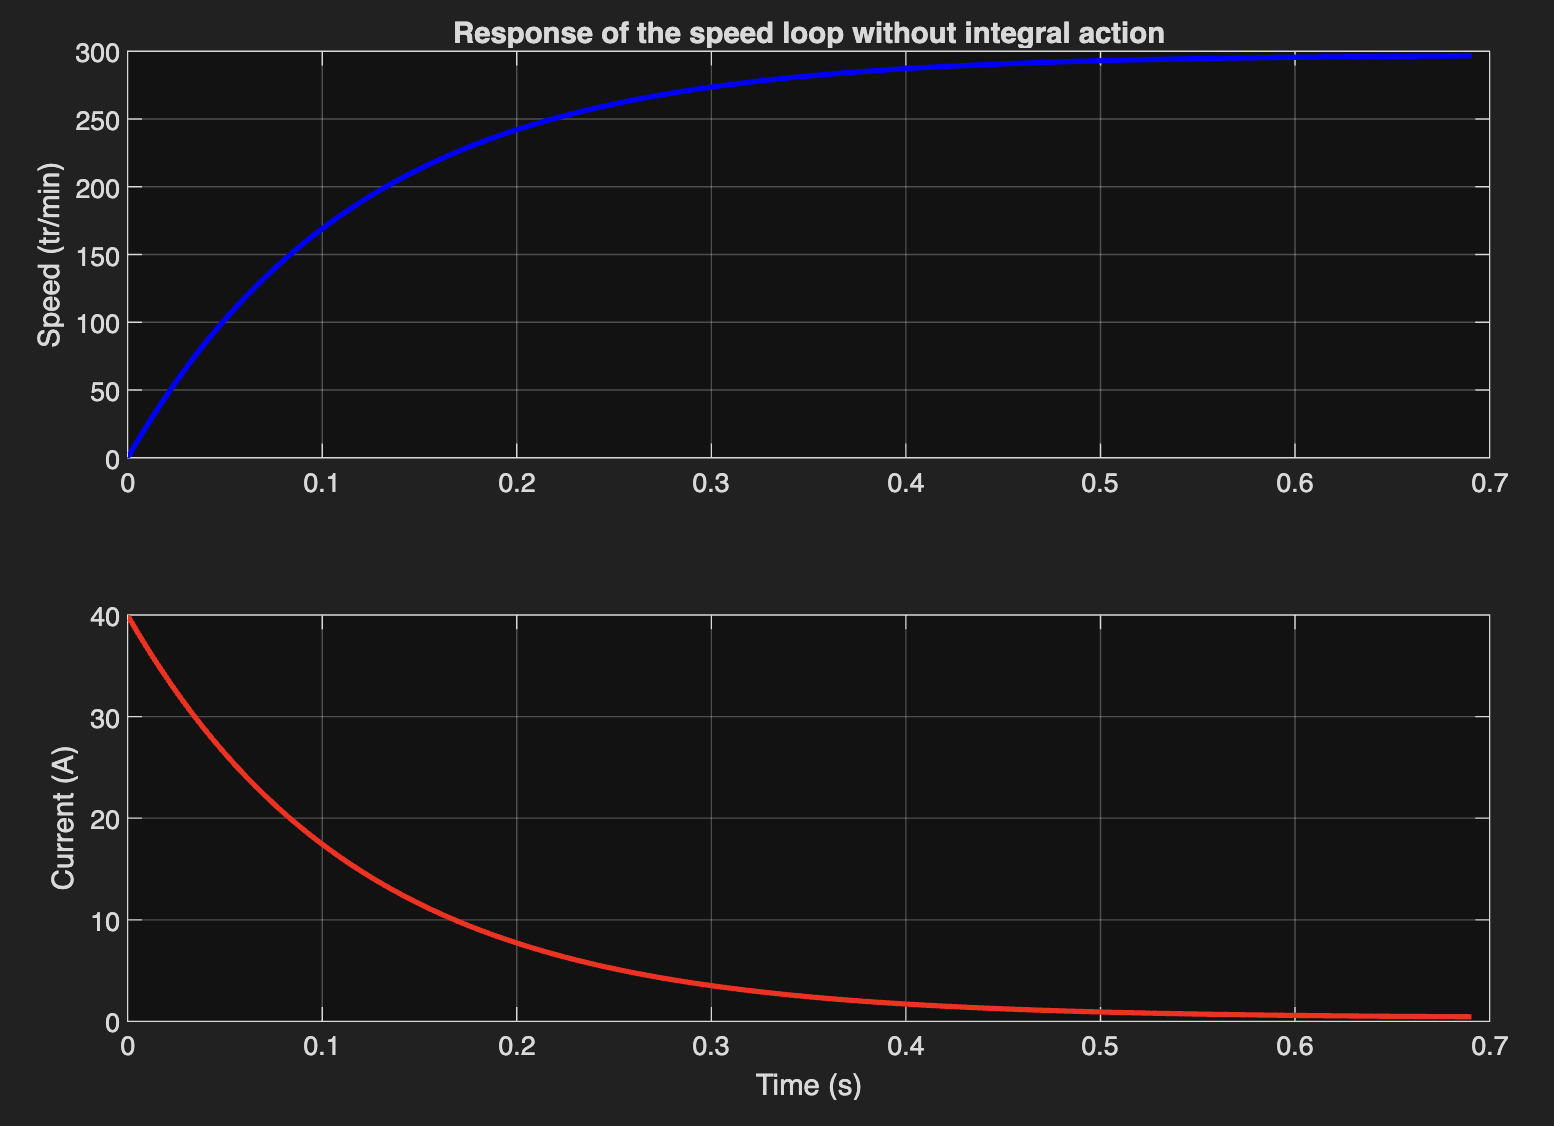
\includegraphics[width=0.85\linewidth]{figures/speedloop.png}
    \caption{Step response of the speed loop with proportional control only.}
    \label{fig:speedloop_no_integral}
\end{figure}

\noindent\textbf{Interpretation of results:}
\begin{itemize}
    \item The speed increases smoothly to the reference of 300~r/min with no overshoot.
    \item The current decreases exponentially as the speed rises, consistent with motor dynamics.
    \item The system behaves as a first-order response with a short settling time (less than 0.7~s).
\end{itemize}

The proportional control ensures a stable response, but a small steady-state error remains due to the lack of integral action.
\subsubsection{Steady-state error with proportional control only}

With proportional speed control and the compensation of $C_r$ disabled, the closed-loop is first order and exhibits a non-zero steady-state error composed of:
(i) a term \emph{independent} of $C_r$ (due to finite loop gain), which decreases as $K_{\Omega p}$ increases but cannot be fully cancelled; and
(ii) a term \emph{proportional} to $C_r$, which requires explicit compensation (see 2.4.d). \,

\paragraph{Numerical evaluation (no disturbance, $C_r=0$).}
For a speed reference of $300\,\mathrm{rpm}$, the MATLAB computation
\begin{verbatim}
Omega_ss = dcgain(sys_bf_KW) * VWref_amp;  % rad/s
Val_finale = Omega_ss * 30/pi;              % rpm
erreur = 300 - Val_finale;                  % rpm
\end{verbatim}
gives $\Omega_{\text{ss}}=31.1538~\mathrm{rad/s}$, i.e.
\[
\Omega_{\text{ss}} = 31.1538 \cdot \frac{30}{\pi} \approx 297.50~\mathrm{rpm},
\quad
e_{\text{ss}} = 300 - 297.50 \approx \boxed{2.50~\mathrm{rpm}}.
\]

\paragraph{Simulink observations (with $C_r$ compensation \emph{deactivated}).}
Using \texttt{TPVitessePartie24.slx}, remove the link from the \texttt{K\_capI/Kc} block output (disables $C_r$ feedforward):
\begin{itemize}
  \item \textbf{Nominal gain} $K_{\Omega p}$: the response tracks $300\,\mathrm{rpm}$ with a small residual offset $\approx 2.5\,\mathrm{rpm}$; see Fig.~\ref{fig:kw}.
  \item \textbf{Halved gain} $K_{\Omega p}/2$: the steady-state error increases and the response slows down (error scales roughly inversely with the proportional gain); see Fig.~\ref{fig:kwdiv2}.
  \item When $C_r$ steps from $0$ to $5~\mathrm{N\,m}$ at $t=10\,\mathrm{s}$, a permanent offset appears (the second error term), confirming the need for the compensation in 2.4.d. \,
\end{itemize}

\begin{figure}[h]
  \centering
  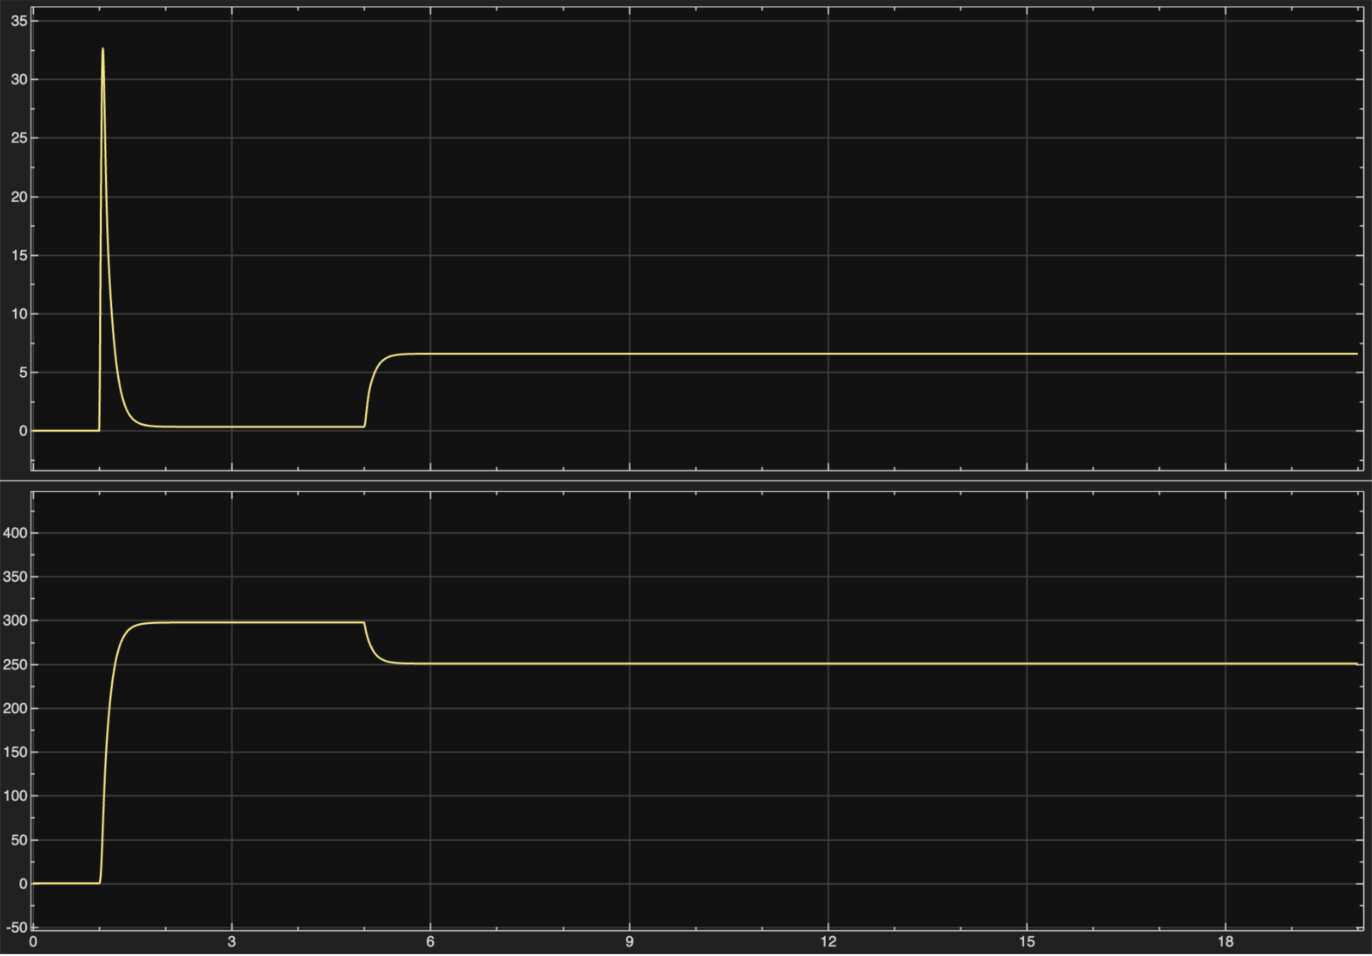
\includegraphics[width=.8\linewidth]{figures/kw}
  \caption{Speed response with $K_{\Omega p}$ (compensation disabled).}
  \label{fig:kw}
\end{figure}

\begin{figure}[h]
  \centering
  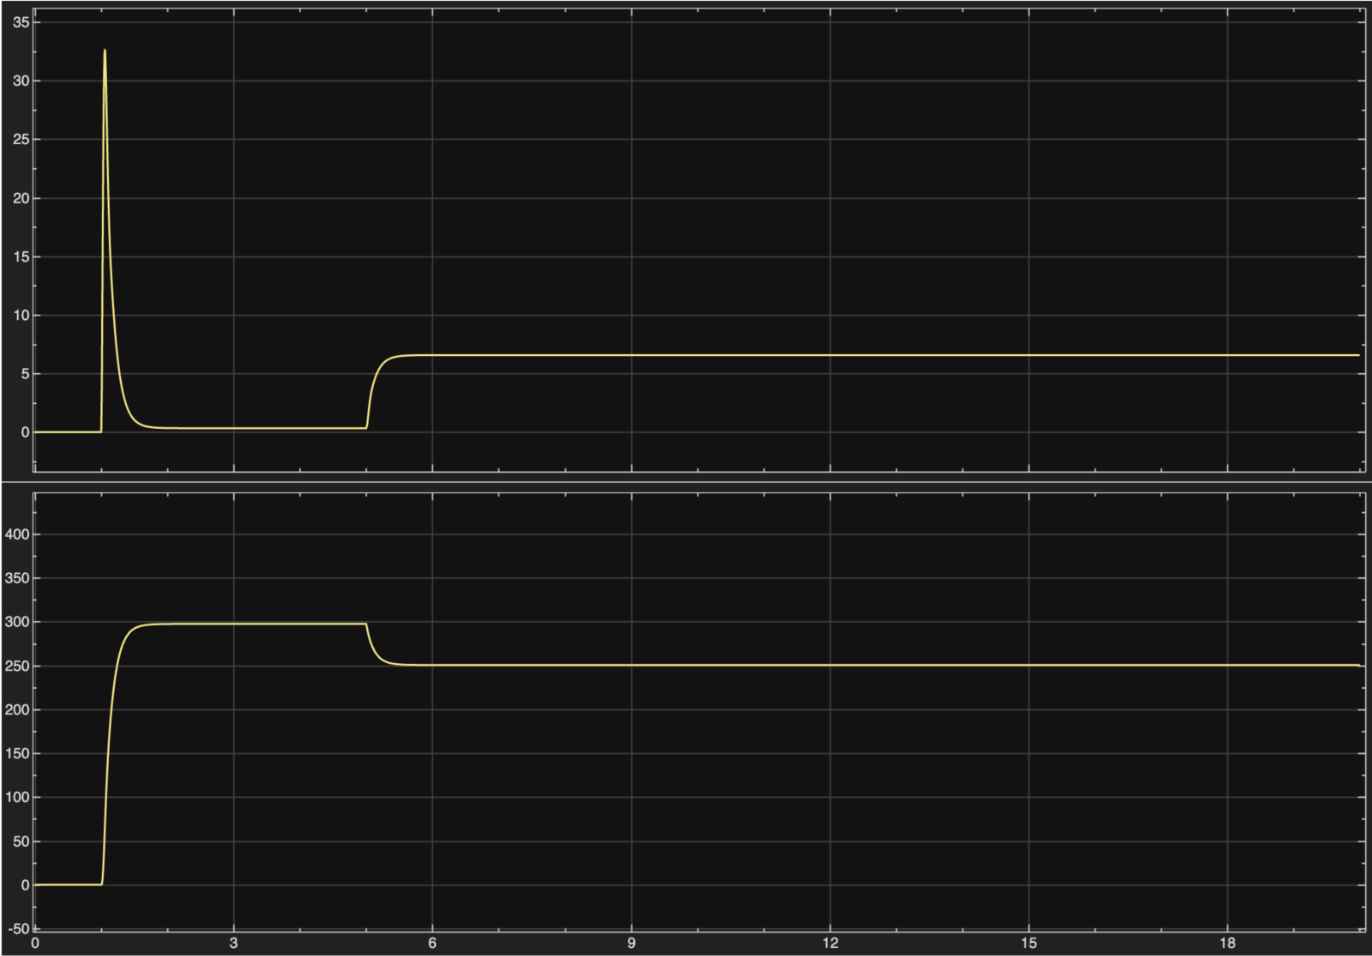
\includegraphics[width=.8\linewidth]{figures/kwdiv2}
  \caption{Speed response with $K_{\Omega p}/2$ (compensation disabled).}
  \label{fig:kwdiv2}
\end{figure}

\subsubsection{Feed-forward compensation of $C_r(t)$ from $\hat C_r$}

\paragraph{Proposed structure.}
Keep the proportional speed loop and add a feed-forward from the estimated resistant torque:
\[
V_I^\ast(t)\;=\;K_{\Omega p}\bigl(V_\Omega^\ast(t)-V_\Omega(t)\bigr)\;+\;K_{\hat C_r}\,\hat C_r(t),
\]
i.e.\ insert a summing junction at the input of the current loop that adds the signal
$\hat C_r$ after a static gain $K_{\hat C_r}$. This is exactly the structure hinted in the subject (Fig.~16). \,

\paragraph{Proof of disturbance cancellation.}
Under the ideal current loop assumption ($I^\ast = V_I^\ast/K_{\text{cap}I}$), the speed dynamics are
\[
J\dot\Omega \;=\; K_c I^\ast - C_r - f\Omega
\;=\; \frac{K_c}{K_{\text{cap}I}}\,V_I^\ast - C_r - f\Omega .
\]
Substituting the proposed $V_I^\ast$:
\[
J\dot\Omega = \frac{K_c}{K_{\text{cap}I}}\,K_{\Omega p}(V_\Omega^\ast - V_\Omega)
\;+\;\frac{K_c}{K_{\text{cap}I}}\,K_{\hat C_r}\,\hat C_r
\;-\; C_r \;-\; f\Omega .
\]
Group the terms driven by the (true) disturbance:
\[
J\dot\Omega = \cdots \;+\;\Bigl(\frac{K_c}{K_{\text{cap}I}}\,K_{\hat C_r}\,\hat C_r - C_r\Bigr) \;-\; f\Omega .
\]
If the observer is exact ($\hat C_r = C_r$), the disturbance channel disappears when
\[
\frac{K_c}{K_{\text{cap}I}}\,K_{\hat C_r} = 1 
\quad \Longleftrightarrow \quad
\boxed{\,K_{\hat C_r} = \dfrac{K_{\text{cap}I}}{K_c}\,}.
\]
Therefore the influence of $C_r(t)$ on $\Omega(t)$ is cancelled with this choice, as required. \,

\paragraph{Remark on estimation error.}
If $\hat C_r = C_r - e_{C_r}$, the residual input is $-(1/J)\,e_{C_r}$, so perfect cancellation occurs when the observer is accurate; otherwise the steady-state error scales with the estimation error.

\paragraph{Implementation note (Simulink).}
Enable the feed-forward path from $\hat C_r$ to $V_I^\ast$ through a gain block fixed at
$K_{\text{cap}I}/K_c$ (the \texttt{K\_capI/Kc} block in \texttt{TPVitessePartie24.slx}). This addition is static feed-forward and does not change the closed-loop poles; it only removes the steady-state disturbance channel (subject to saturation limits). \,

\subsubsection{Validation of steady-state error cancellation (with $\hat C_r$ feed-forward)}

With the compensation enabled (connecting the block \texttt{K\_capI/Kc} so that $K_{\hat C_r}=K_{\text{cap}I}/K_c$), the command is
\[
V_I^\ast(t)=K_{\Omega p}\bigl(V_\Omega^\ast(t)-V_\Omega(t)\bigr)+\frac{K_{\text{cap}I}}{K_c}\,\hat C_r(t),
\]
which cancels the disturbance channel under the ideal current loop assumption. \,

\paragraph{Simulation scenario.}
In \texttt{TPVitessePartie24.slx}, we apply a speed step $\Omega^\ast:0\!\to\!300~\mathrm{rpm}$ at $t=1\,\mathrm{s}$ and a load step $C_r:0\!\to\!5~\mathrm{N\,m}$ at $t=5\,\mathrm{s}$. The current and speed responses are shown in Fig.~\ref{fig:kcplugged}.

\paragraph{Results.}
\begin{itemize}
  \item Before the disturbance, $\Omega(t)$ reaches $300~\mathrm{rpm}$ with negligible offset.
  \item At $t=5\,\mathrm{s}$, the load step produces a short transient (small dip), after which $\Omega(t)$ returns to the reference with \emph{zero} steady-state error (numerically $<0.1\%$).
  \item The current settles to the value needed to balance the load, $I_\infty \approx C_r/K_c$; for $C_r=5~\mathrm{N\,m}$ and $K_c\simeq0.795$, this gives $I_\infty\!\approx\!6.3~\mathrm{A}$, consistent with the plot.
\end{itemize}

\paragraph{Conclusion.}
Activating the feed-forward $\hat C_r$ with $K_{\hat C_r}=K_{\text{cap}I}/K_c$ removes the steady-state error of $\Omega(t)$ with respect to $\Omega^\ast(t)$ despite the load step, as predicted by the analysis in 2.4.d. \,

\begin{figure}[h]
  \centering
  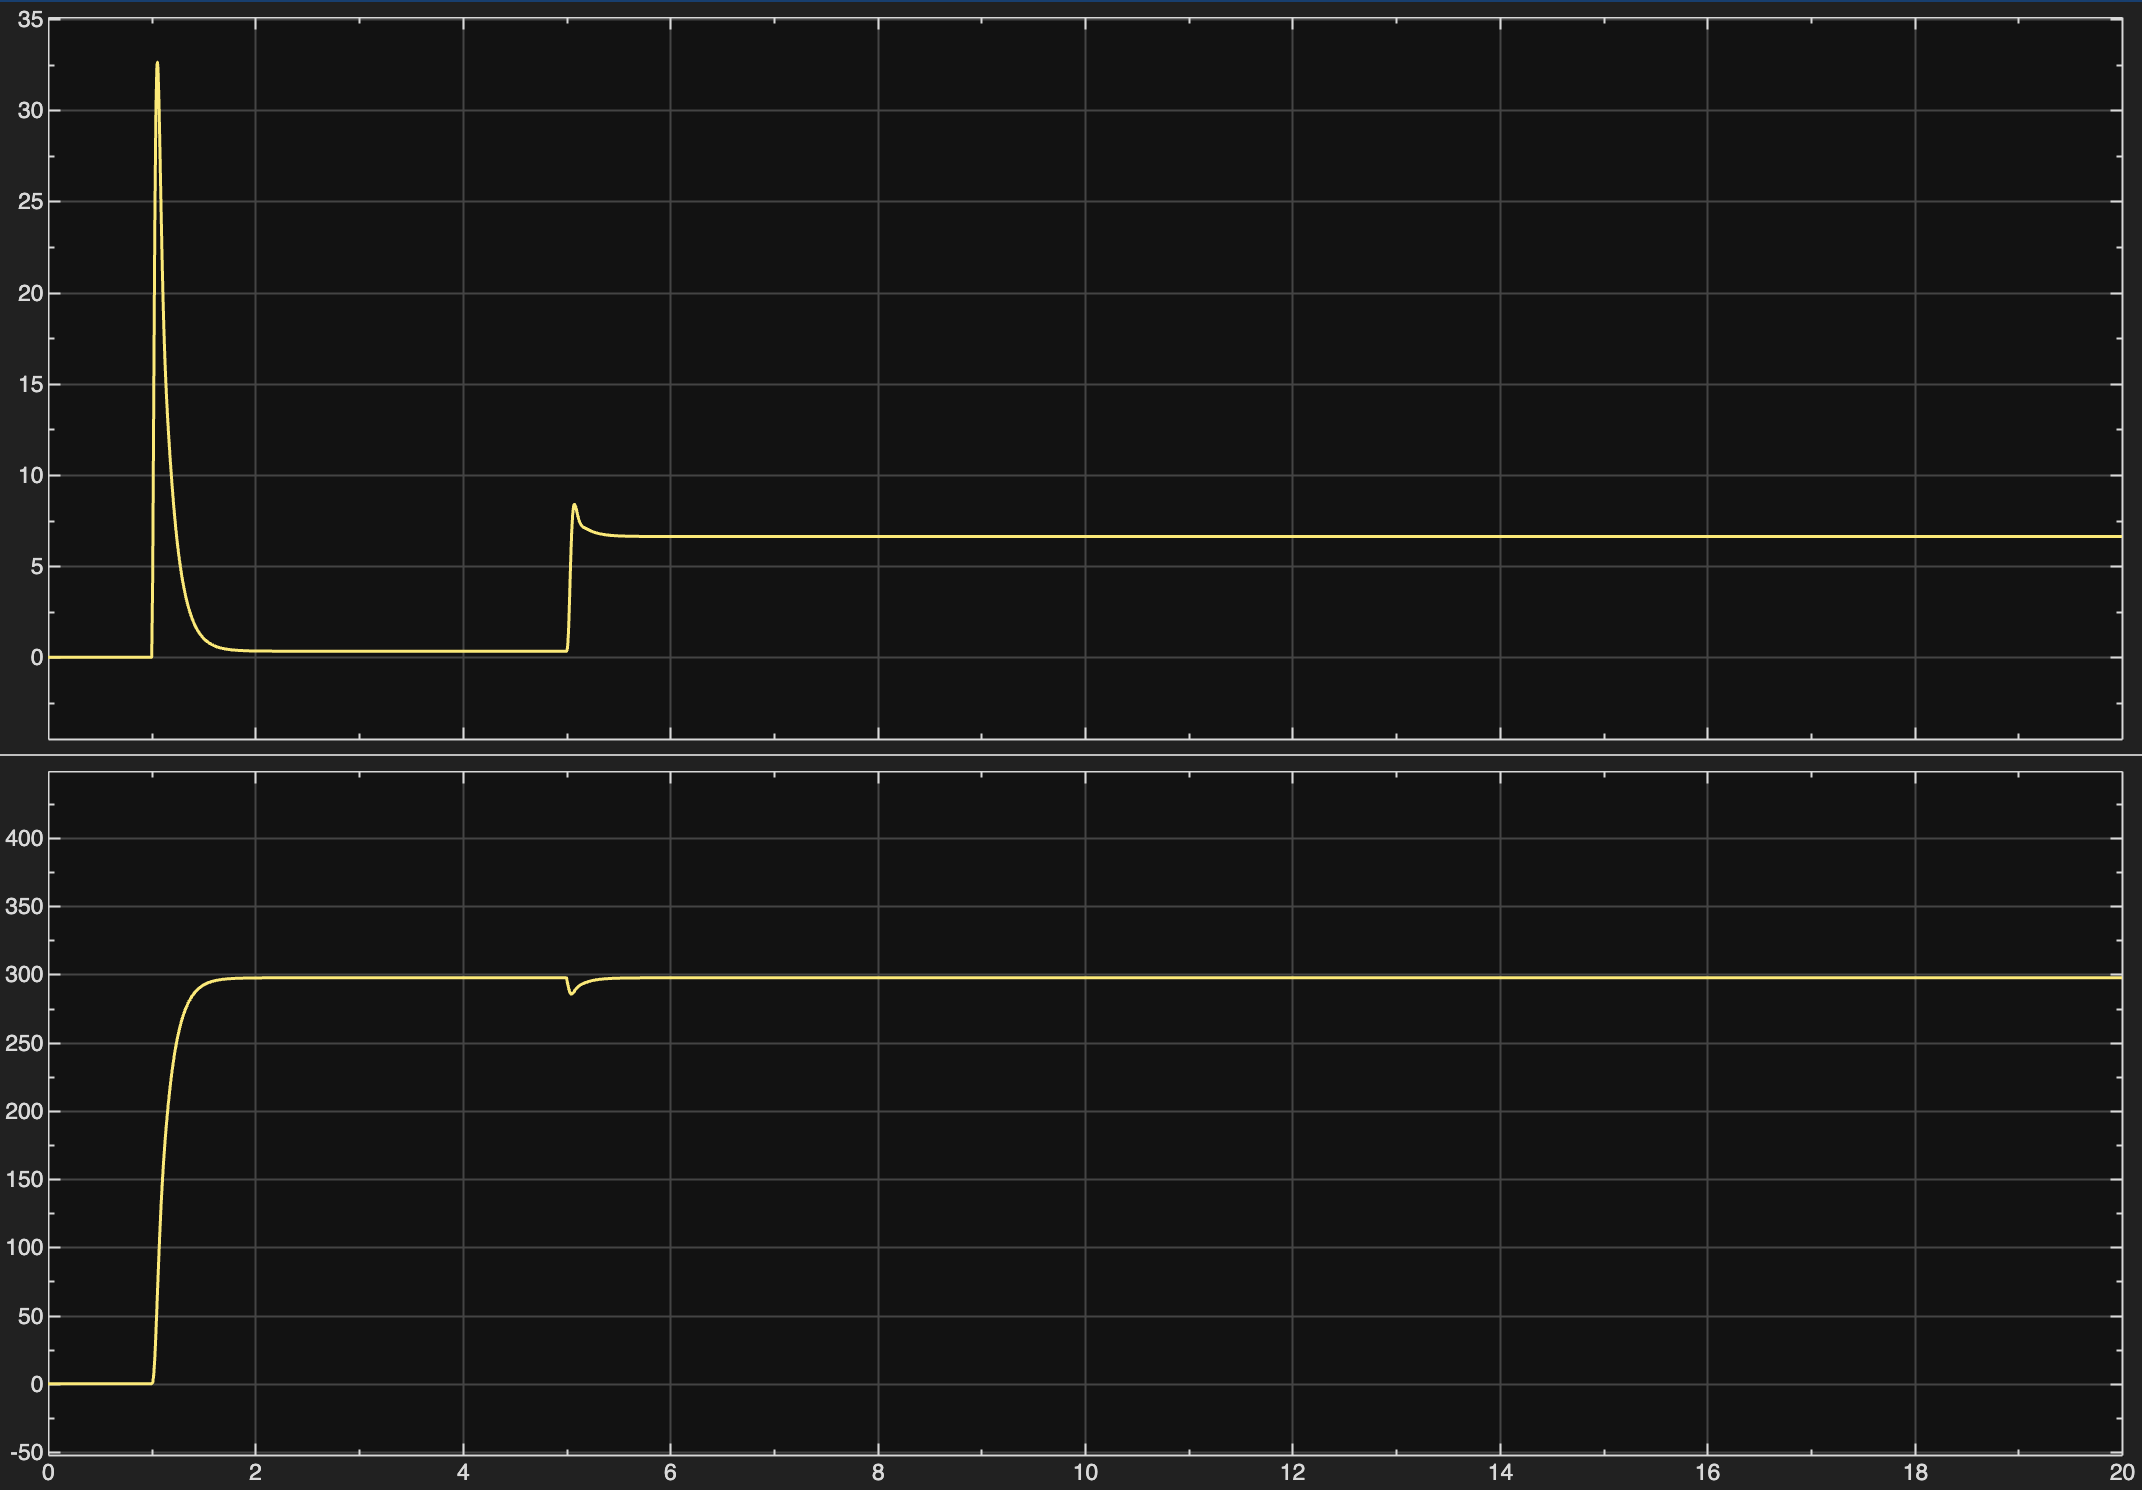
\includegraphics[width=.95\linewidth]{figures/kcplugged.png}
  \caption{Effect of enabling the static compensation $K_{\hat C_r}=K_{\text{cap}I}/K_c$ using $\hat C_r(t)$ from the observer: the steady-state error due to a $C_r$ step is eliminated while preserving the transient performance.}
  \label{fig:kcplugged}
\end{figure}

\newpage
%------------ Section 3 ----------------

\section{Experimental Validation of the Controllers}

\label{sec:exp}

This section reports the laboratory validation of the controllers designed in Part~2. 
Several Simulink configurations were used successively (current loop, speed loop, and finally the observer). 
Due to limited laboratory time, \textbf{only the final implementation corresponding to the observer (Part~3.3) was saved as a representative Simulink diagram}. 
However, \textbf{all measurement results} obtained at each step were recorded and are presented below to assess the performance of every loop. 
Earlier configurations for the current and speed control followed the same structure as the final one (inner current loop, outer speed loop, voltage saturation, and acquisition blocks).

\vspace{4pt}
\noindent\textit{Practical constraints.} For hardware safety, the armature current was limited to 20~A, voltage commands were saturated at $\pm9$~V, and step amplitudes were increased gradually to avoid excessive mechanical stress and large current transients.

%-------------------- 3.1 --------------------
\subsection{Current Regulation Experiment}

The experimental results of the current control loop are shown in Figure~\ref{fig:exp_I_20A}. 
The upper plot displays the armature current (\textit{courant}) and the lower plot shows the corresponding motor speed (\textit{vitesse}). 
Several step changes were applied to the current reference, increasing successively from approximately 1~A to 2~A, 3~A and finally 10~A. 
The current follows the reference with a fast transient and negligible overshoot, demonstrating a well-tuned inner current loop. 
Small fluctuations in the measured signal are mainly due to sensor noise. 
The motor speed evolves consistently with the current variations, rising up to about 1000~rpm and then decreasing when the current is reduced or reversed. 
This confirms the expected electromechanical coupling between torque and speed. 
At the end of the experiment, both current and speed return smoothly to zero when the converter command is disabled.

\begin{figure}[H]
    \centering
    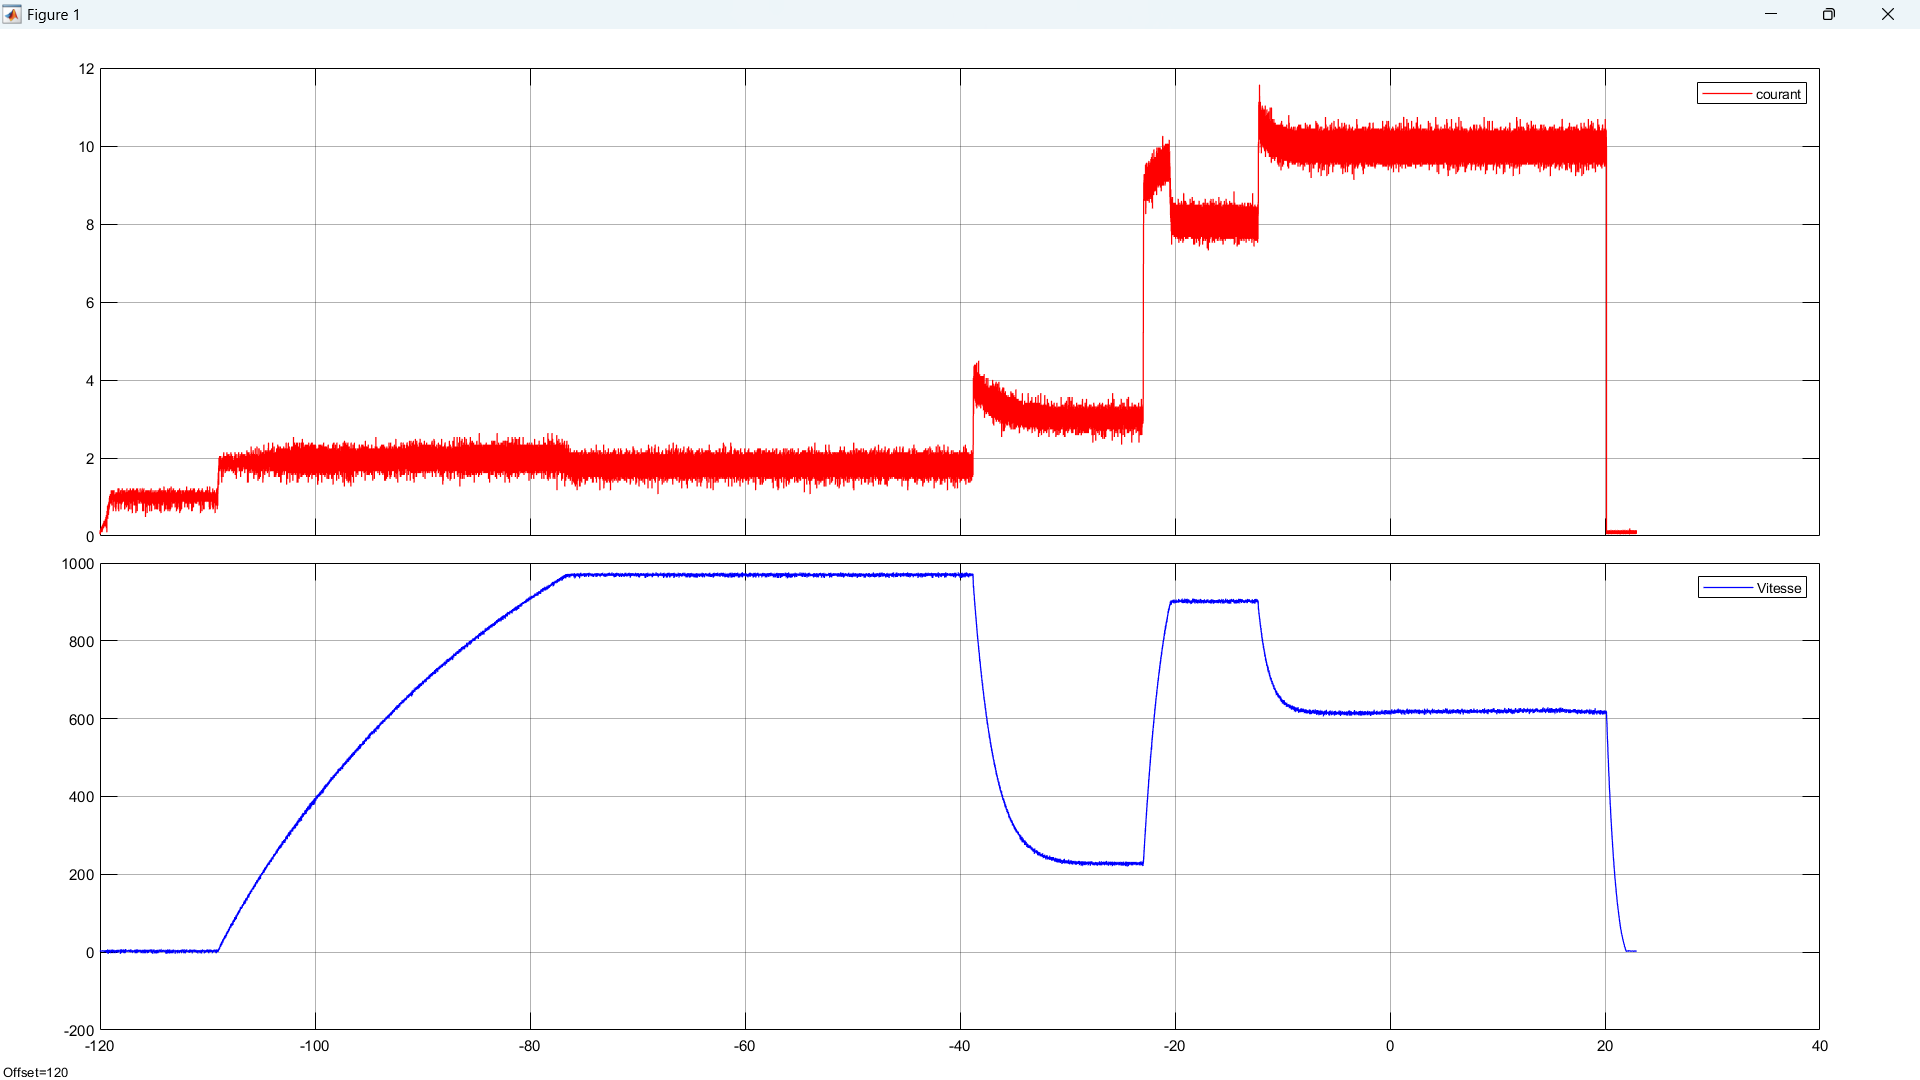
\includegraphics[width=\linewidth, keepaspectratio]{figures/PP1.png}
    \caption{Measured current (top, in~A) and speed (bottom, in~rpm) during the current regulation test. 
    The current loop shows fast and stable response with negligible overshoot.}
    \label{fig:exp_I_20A}
\end{figure}


%-------------------- 3.2 --------------------
\subsection{Speed Regulation Experiment}

The experimental validation of the speed controller was performed following the four test scenarios defined in Question~2.2.c. 
For each case, the converter operated in ``Automatic'' mode, and the speed reference $\Omega^*(t)$ was imposed through the control panel. 
The measured motor speed (\textit{vitesse}) and armature current (\textit{courant}) were recorded simultaneously.

\begin{itemize}
    \item $\mathbf{Case~1:}$ $C_r(t)=0$, $\Omega^*(t)$ changes from $0$ to $300~\text{rpm}$ at $t=1~\text{s}$.
    \item $\mathbf{Case~2:}$ $C_r(t)=0$, $\Omega^*(t)$ changes from $0$ to $500~\text{rpm}$ at $t=1~\text{s}$.
    \item $\mathbf{Case~3:}$ $C_r(t)=0$, $\Omega^*(t)$ changes from $0$ to $1200~\text{rpm}$ at $t=1~\text{s}$.
    \item $\mathbf{Case~4:}$ $\Omega^*(t)$ changes from $0$ to $300~\text{rpm}$ at $t=1~\text{s}$, while the resistant torque $C_r(t)$ increases from $0$ to $5~\text{Nm}$ at $t=10~\text{s}$.
\end{itemize}

The measured responses are summarized in Figures~\ref{fig:exp_W_300}--\ref{fig:exp_W_disturbance}. 
In all cases, the speed regulation shows a well-damped transient with limited overshoot and negligible steady-state error. 
For moderate speed commands (300~rpm and 500~rpm), the current peaks remain within the admissible range (below 20~A), confirming that the current limiter effectively constrains the torque demand. 
When the reference is increased to 1200~rpm, the system still converges but the transient becomes slower, illustrating the saturation effect of the voltage converter.

When a disturbance torque of 5~Nm is applied at $t=10~\text{s}$, a brief speed drop is observed, immediately compensated by the integral action of the speed controller. 
The steady-state speed returns to its nominal value within less than one second, demonstrating the robustness of the closed-loop regulation against load disturbances.

\begin{figure}[H]
    \centering
    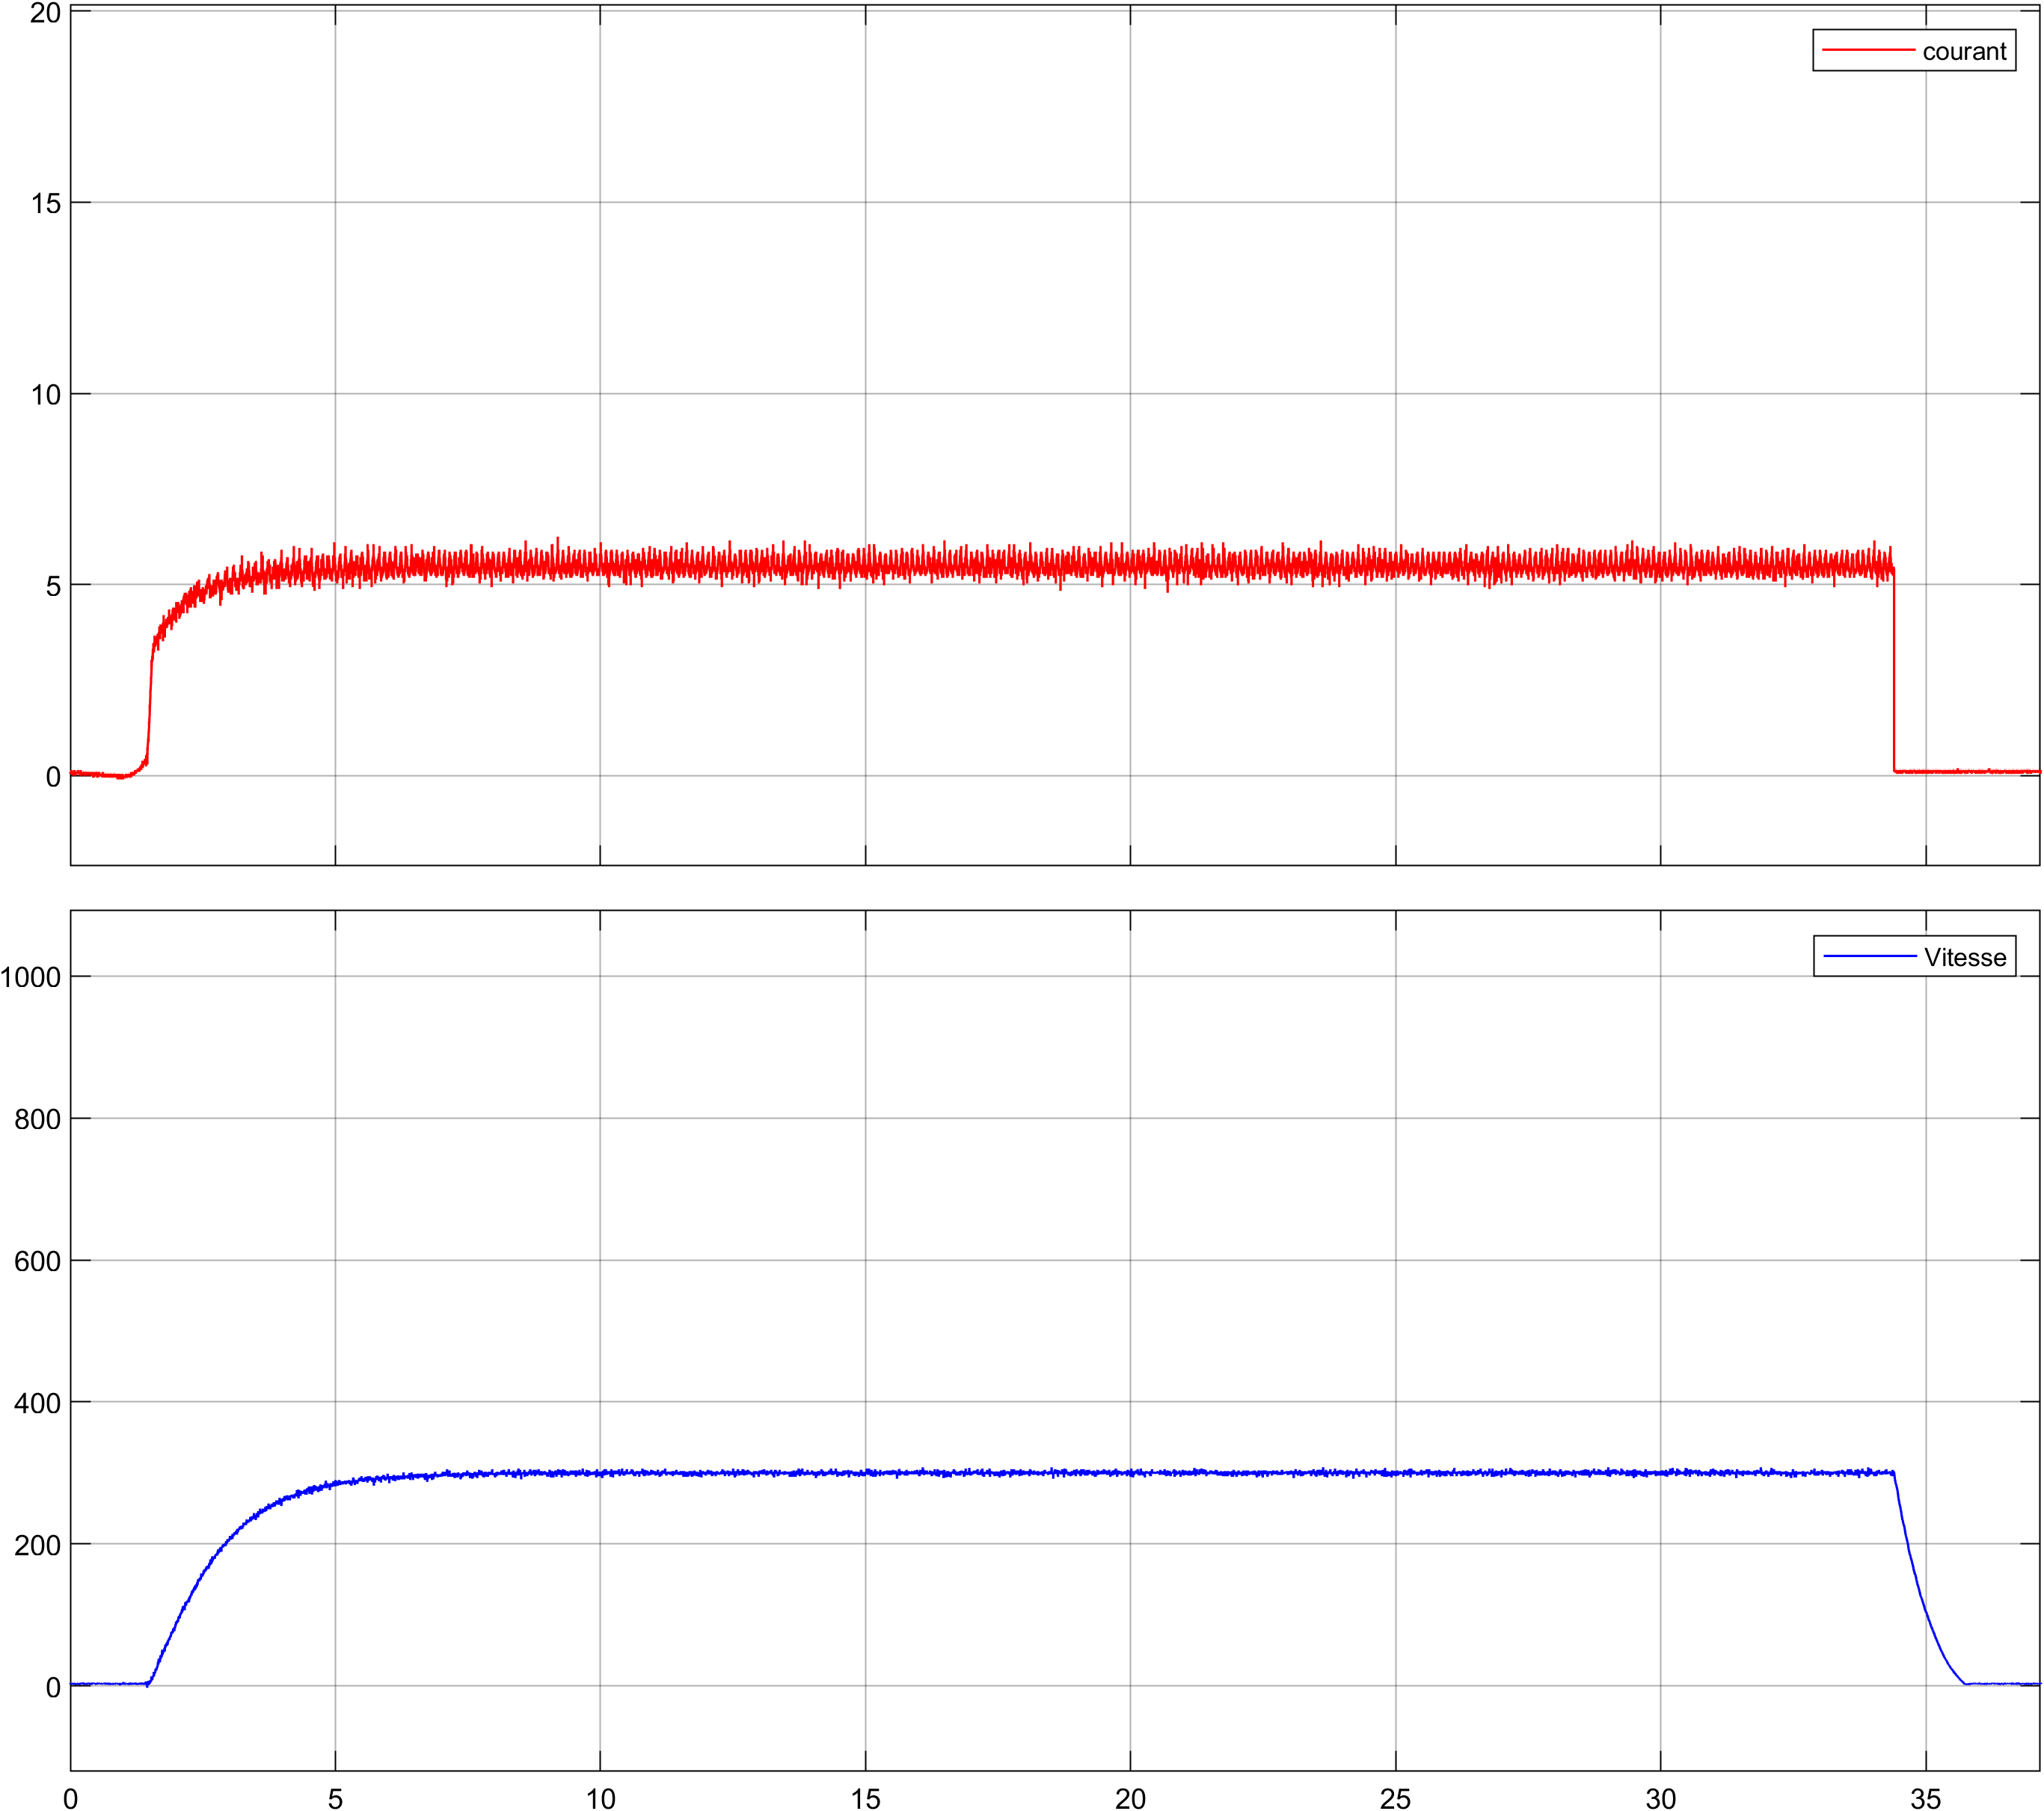
\includegraphics[width=\linewidth, keepaspectratio]{figures/p300.png}
    \caption{Speed loop --- measured response for a $0 \rightarrow 300~\text{rpm}$ reference step.}
    \label{fig:exp_W_300}
\end{figure}

\begin{figure}[H]
    \centering
    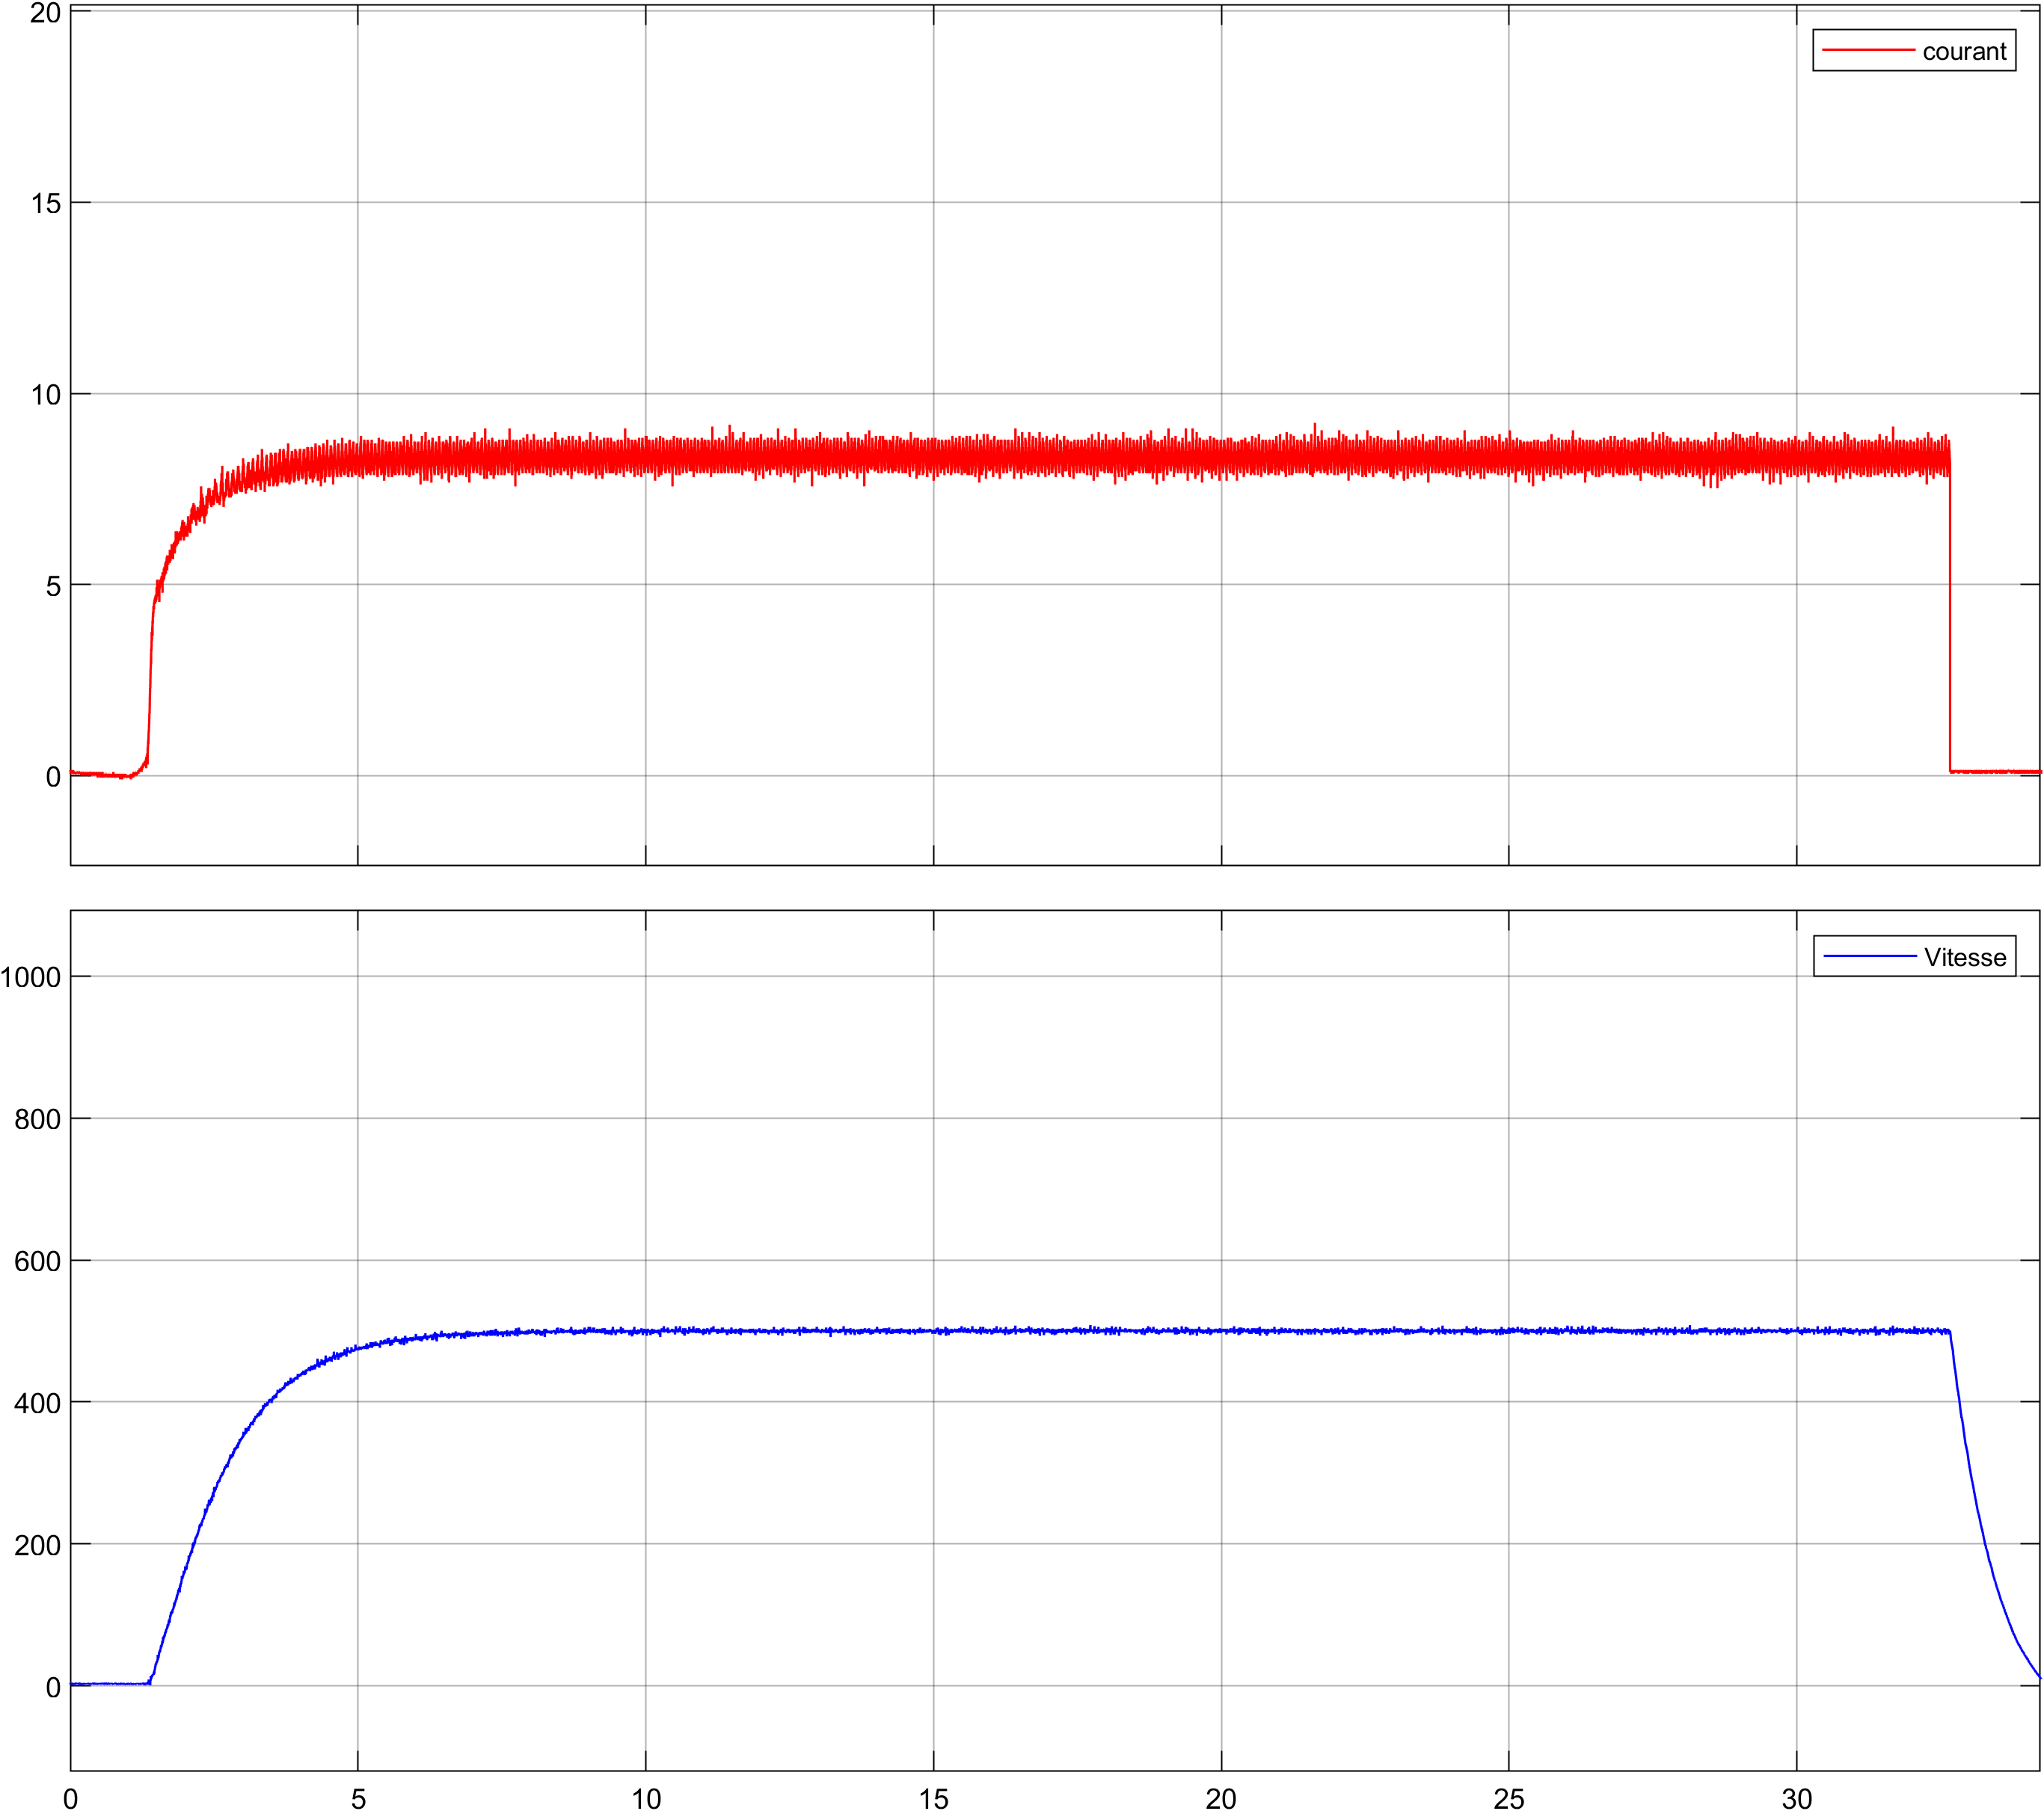
\includegraphics[width=\linewidth, keepaspectratio]{figures/p500.png}
    \caption{Speed loop --- measured response for a $0 \rightarrow 500~\text{rpm}$ reference step.}
    \label{fig:exp_W_500}
\end{figure}

\begin{figure}[H]
    \centering
    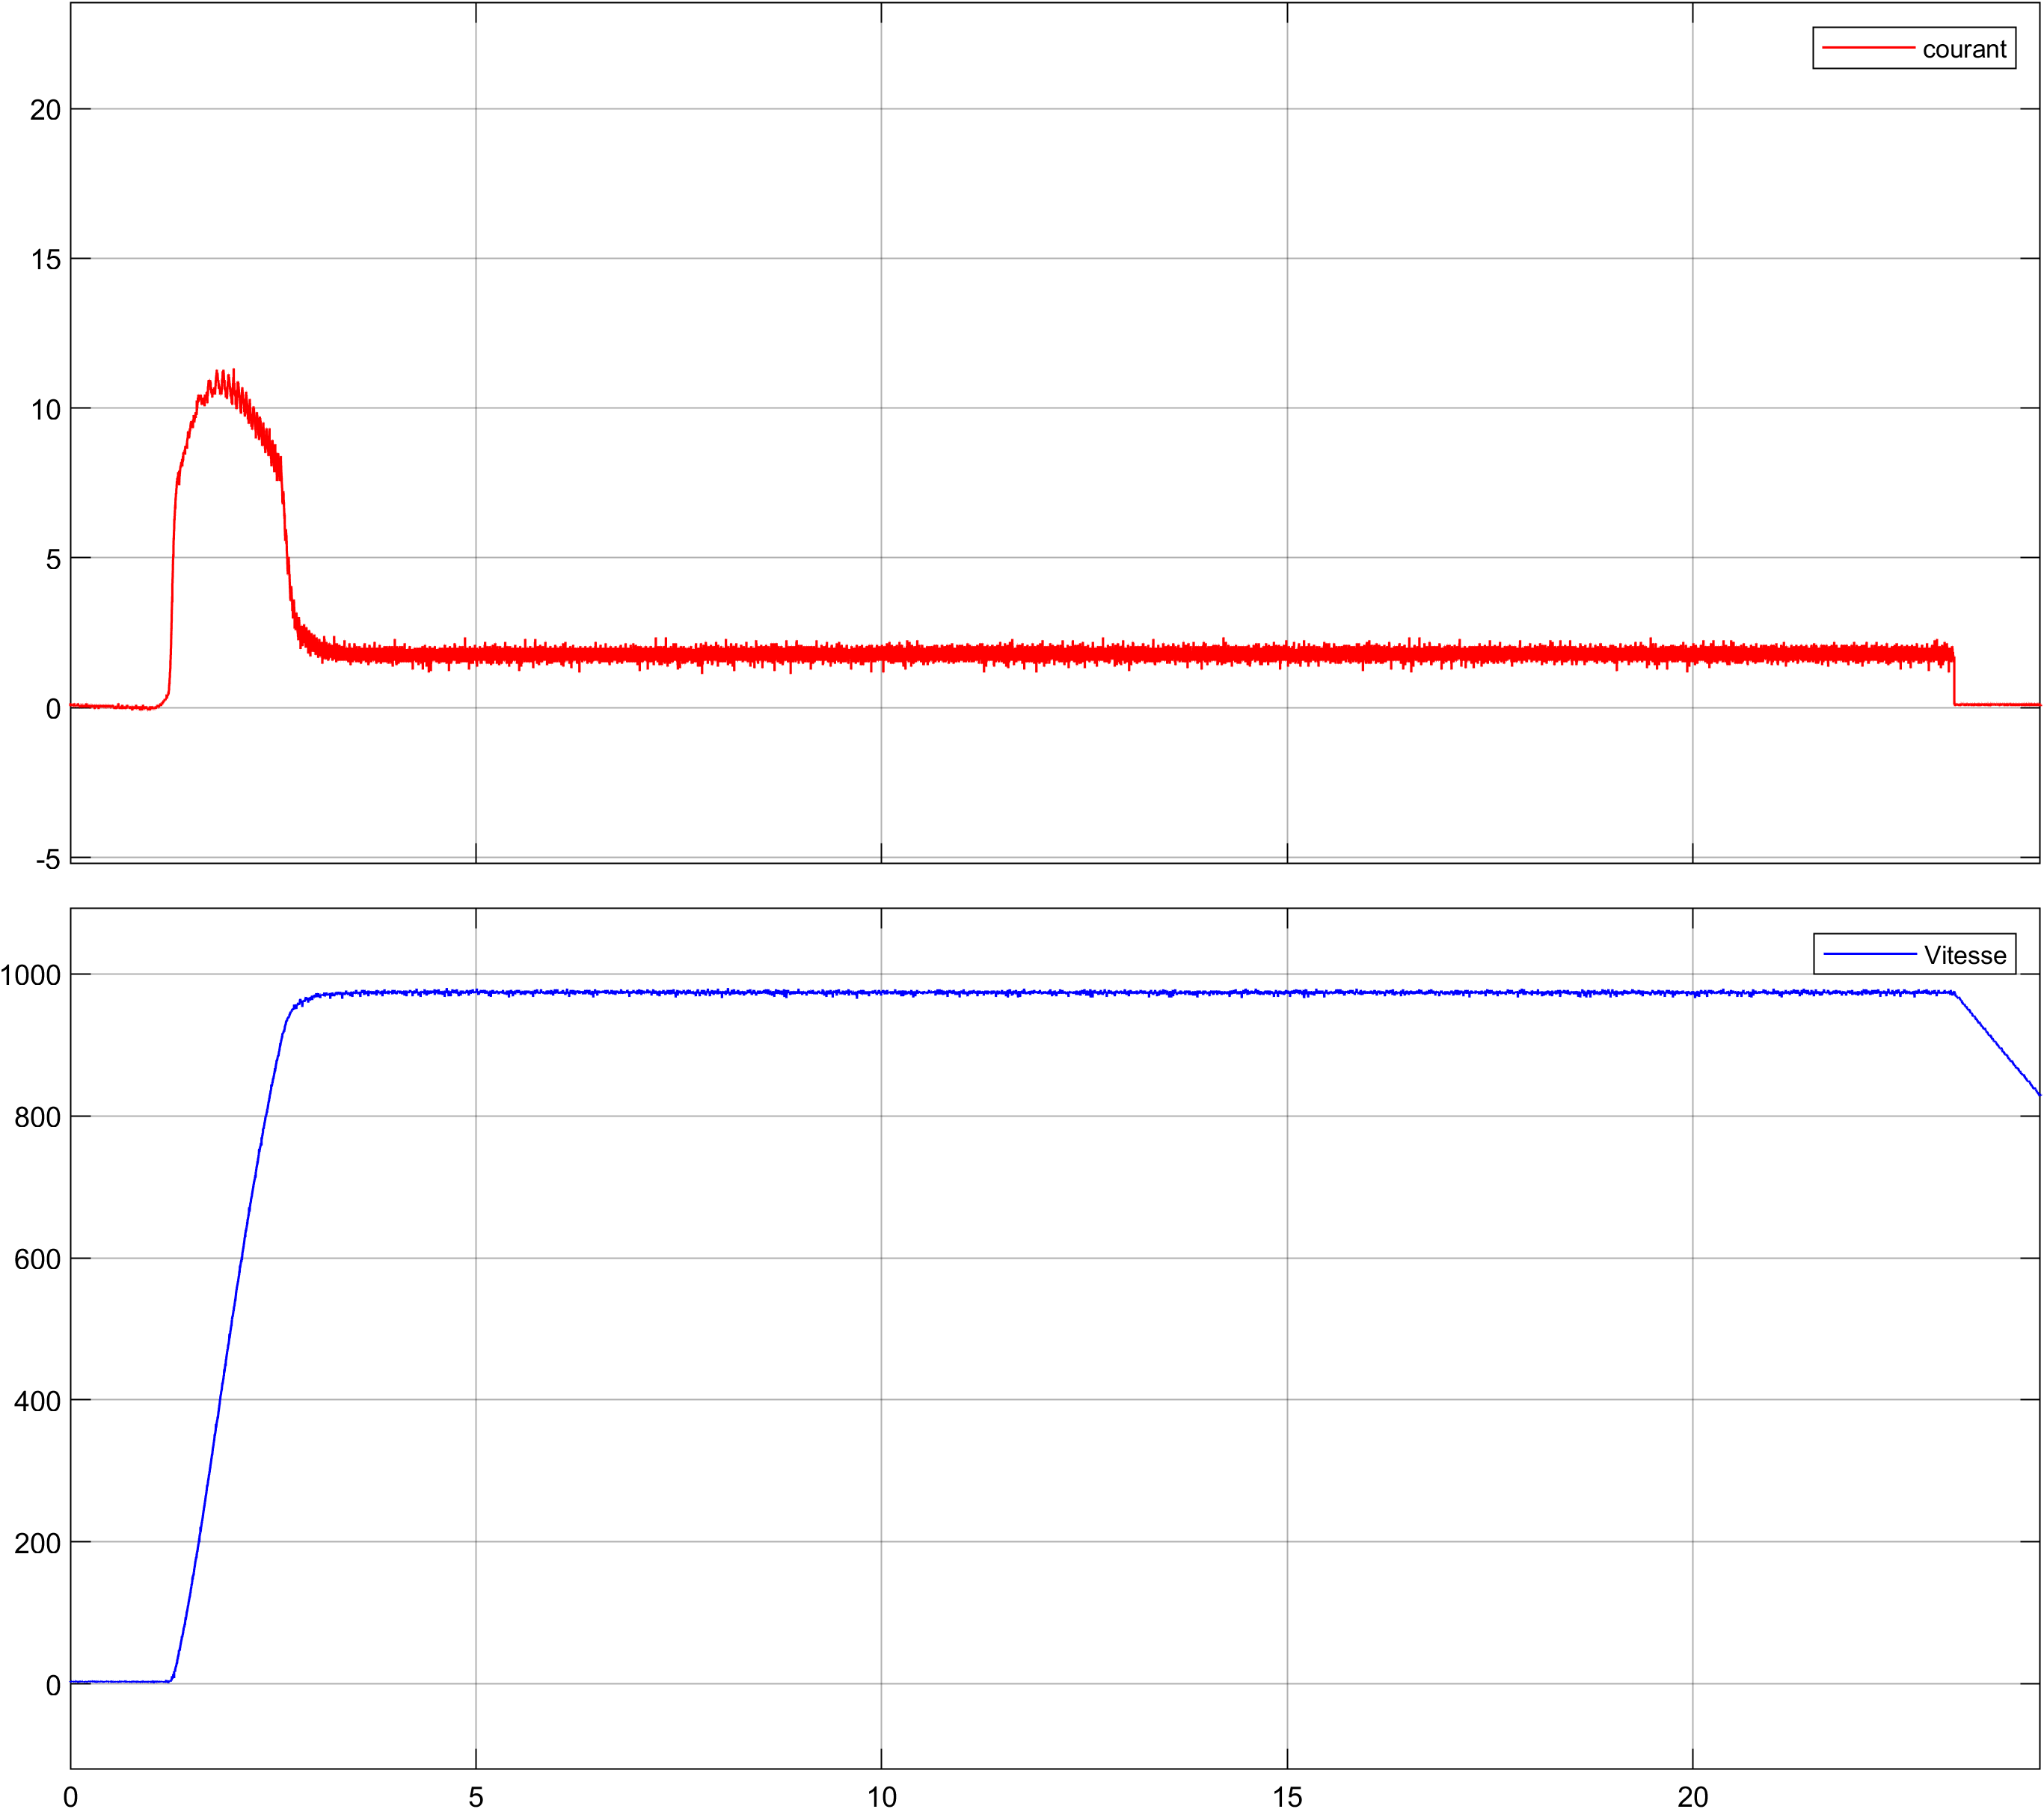
\includegraphics[width=\linewidth, keepaspectratio]{figures/p1200.png}
    \caption{Speed loop --- measured response for a $0 \rightarrow 1200~\text{rpm}$ reference step, showing converter saturation effects.}
    \label{fig:exp_W_1200}
\end{figure}

\begin{figure}[H]
    \centering
    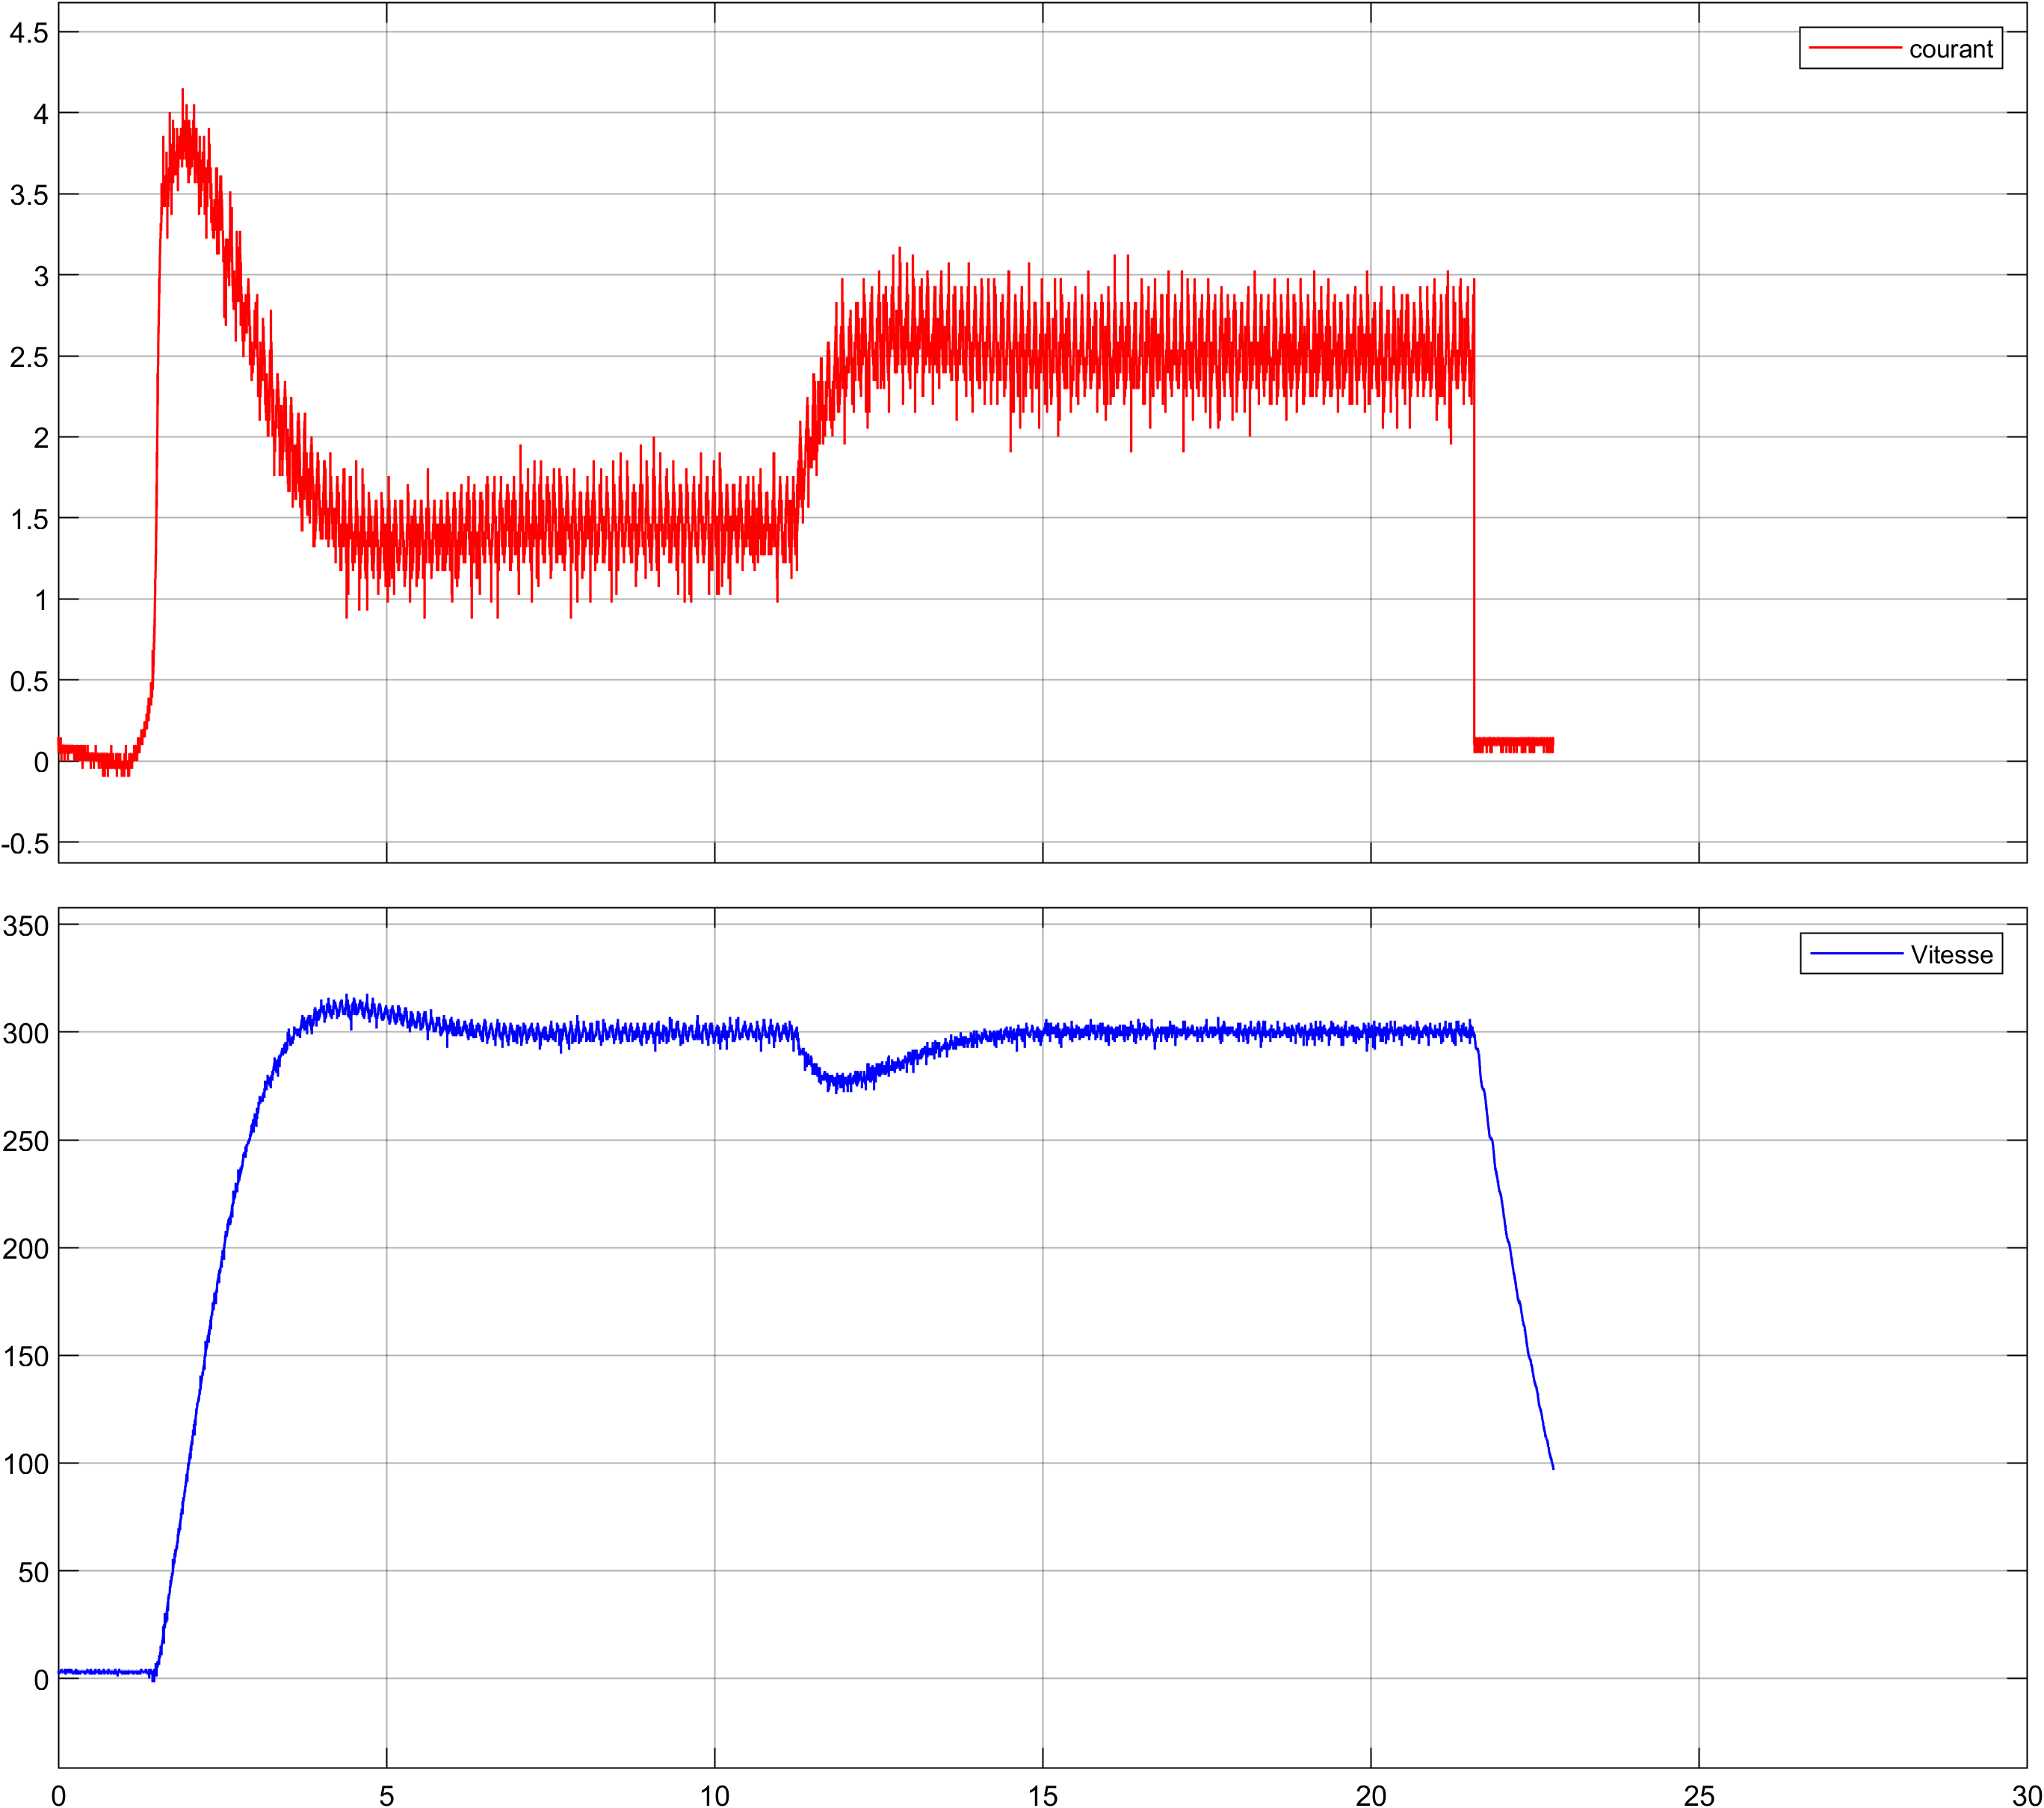
\includegraphics[width=\linewidth, keepaspectratio]{figures/p300cr5.png}
    \caption{Speed loop --- disturbance rejection test: a $5~\text{Nm}$ torque is applied at $t=10~\text{s}$. 
    The controller compensates the perturbation and restores the nominal speed.}
    \label{fig:exp_W_disturbance}
\end{figure}

%-------------------- 3.3 --------------------
\subsection{Observer Implementation and Validation}
\label{subsec:exp_obs}

Finally, the observer developed in Section~2.3 was implemented to estimate the states $[\hat I,\ \hat\Omega,\ \hat C_r]$. 
The \textbf{final Simulink configuration} used for all experiments is shown in Figure~\ref{fig:exp_obs_model}; it summarizes the complete control architecture (inner current loop, outer speed loop, observer, saturation, and I/O blocks).

\begin{figure}[H]
    \centering
    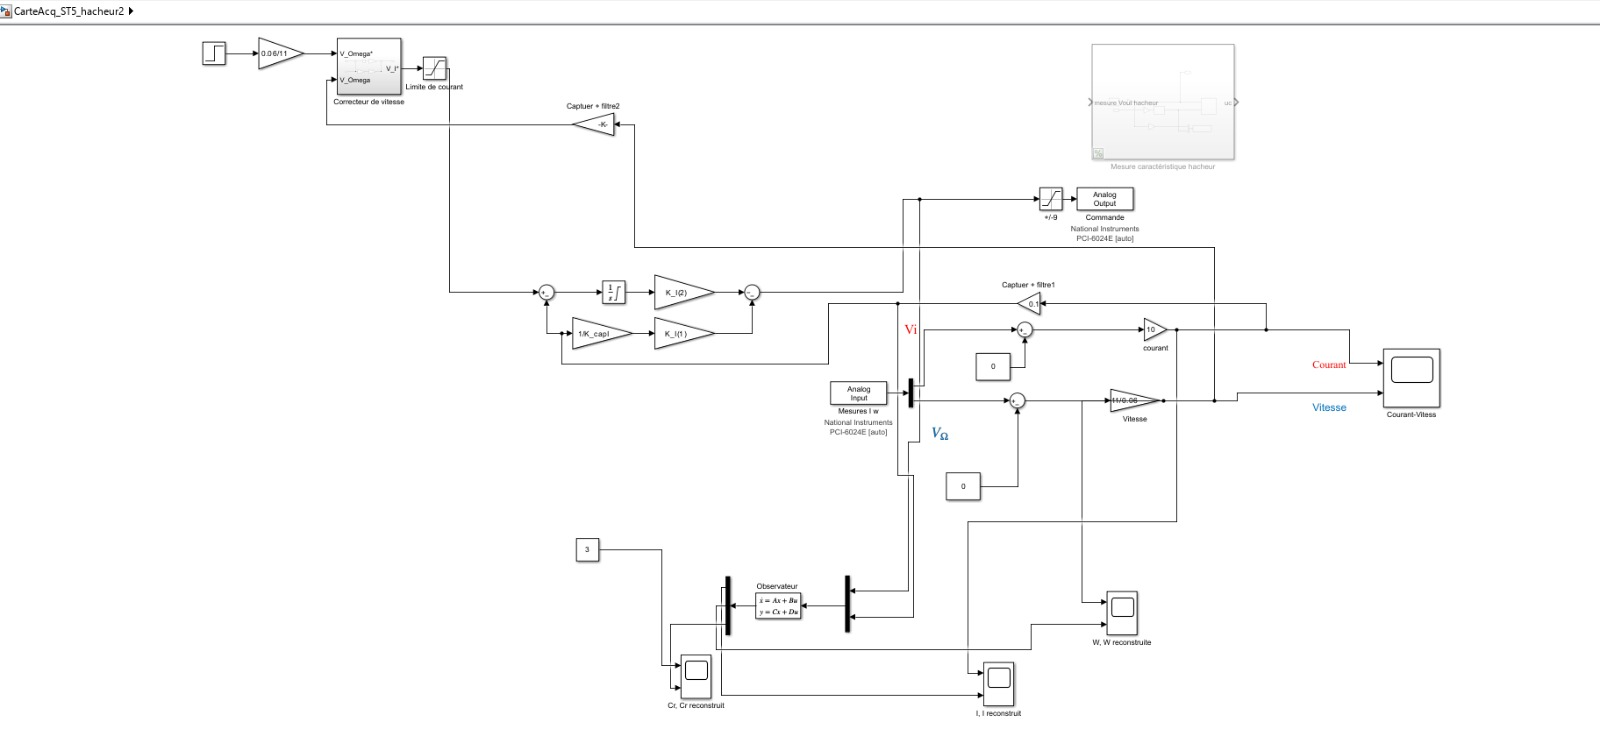
\includegraphics[width=\linewidth, keepaspectratio]{figures/simulink.png}
    \caption{Final Simulink implementation used on the bench (saved during Part~3.3). 
    Earlier configurations for the current and speed loops followed the same structure.}
    \label{fig:exp_obs_model}
\end{figure}

The current estimate converged rapidly and accurately. 
The speed estimate showed small mismatches and high-frequency noise, mainly due to sensor noise and converter nonlinearities. 
When using $\hat C_r$ for proportional disturbance compensation, the closed loop became sensitive to this noise and could lose stability. 
Therefore, compensation based on $\hat C_r$ was not retained on the bench without additional filtering or gain scheduling. 
Figure~\ref{fig:exp_obs_results} illustrates the convergence of the estimated variables towards their measured counterparts.

\begin{figure}[H]
    \centering
    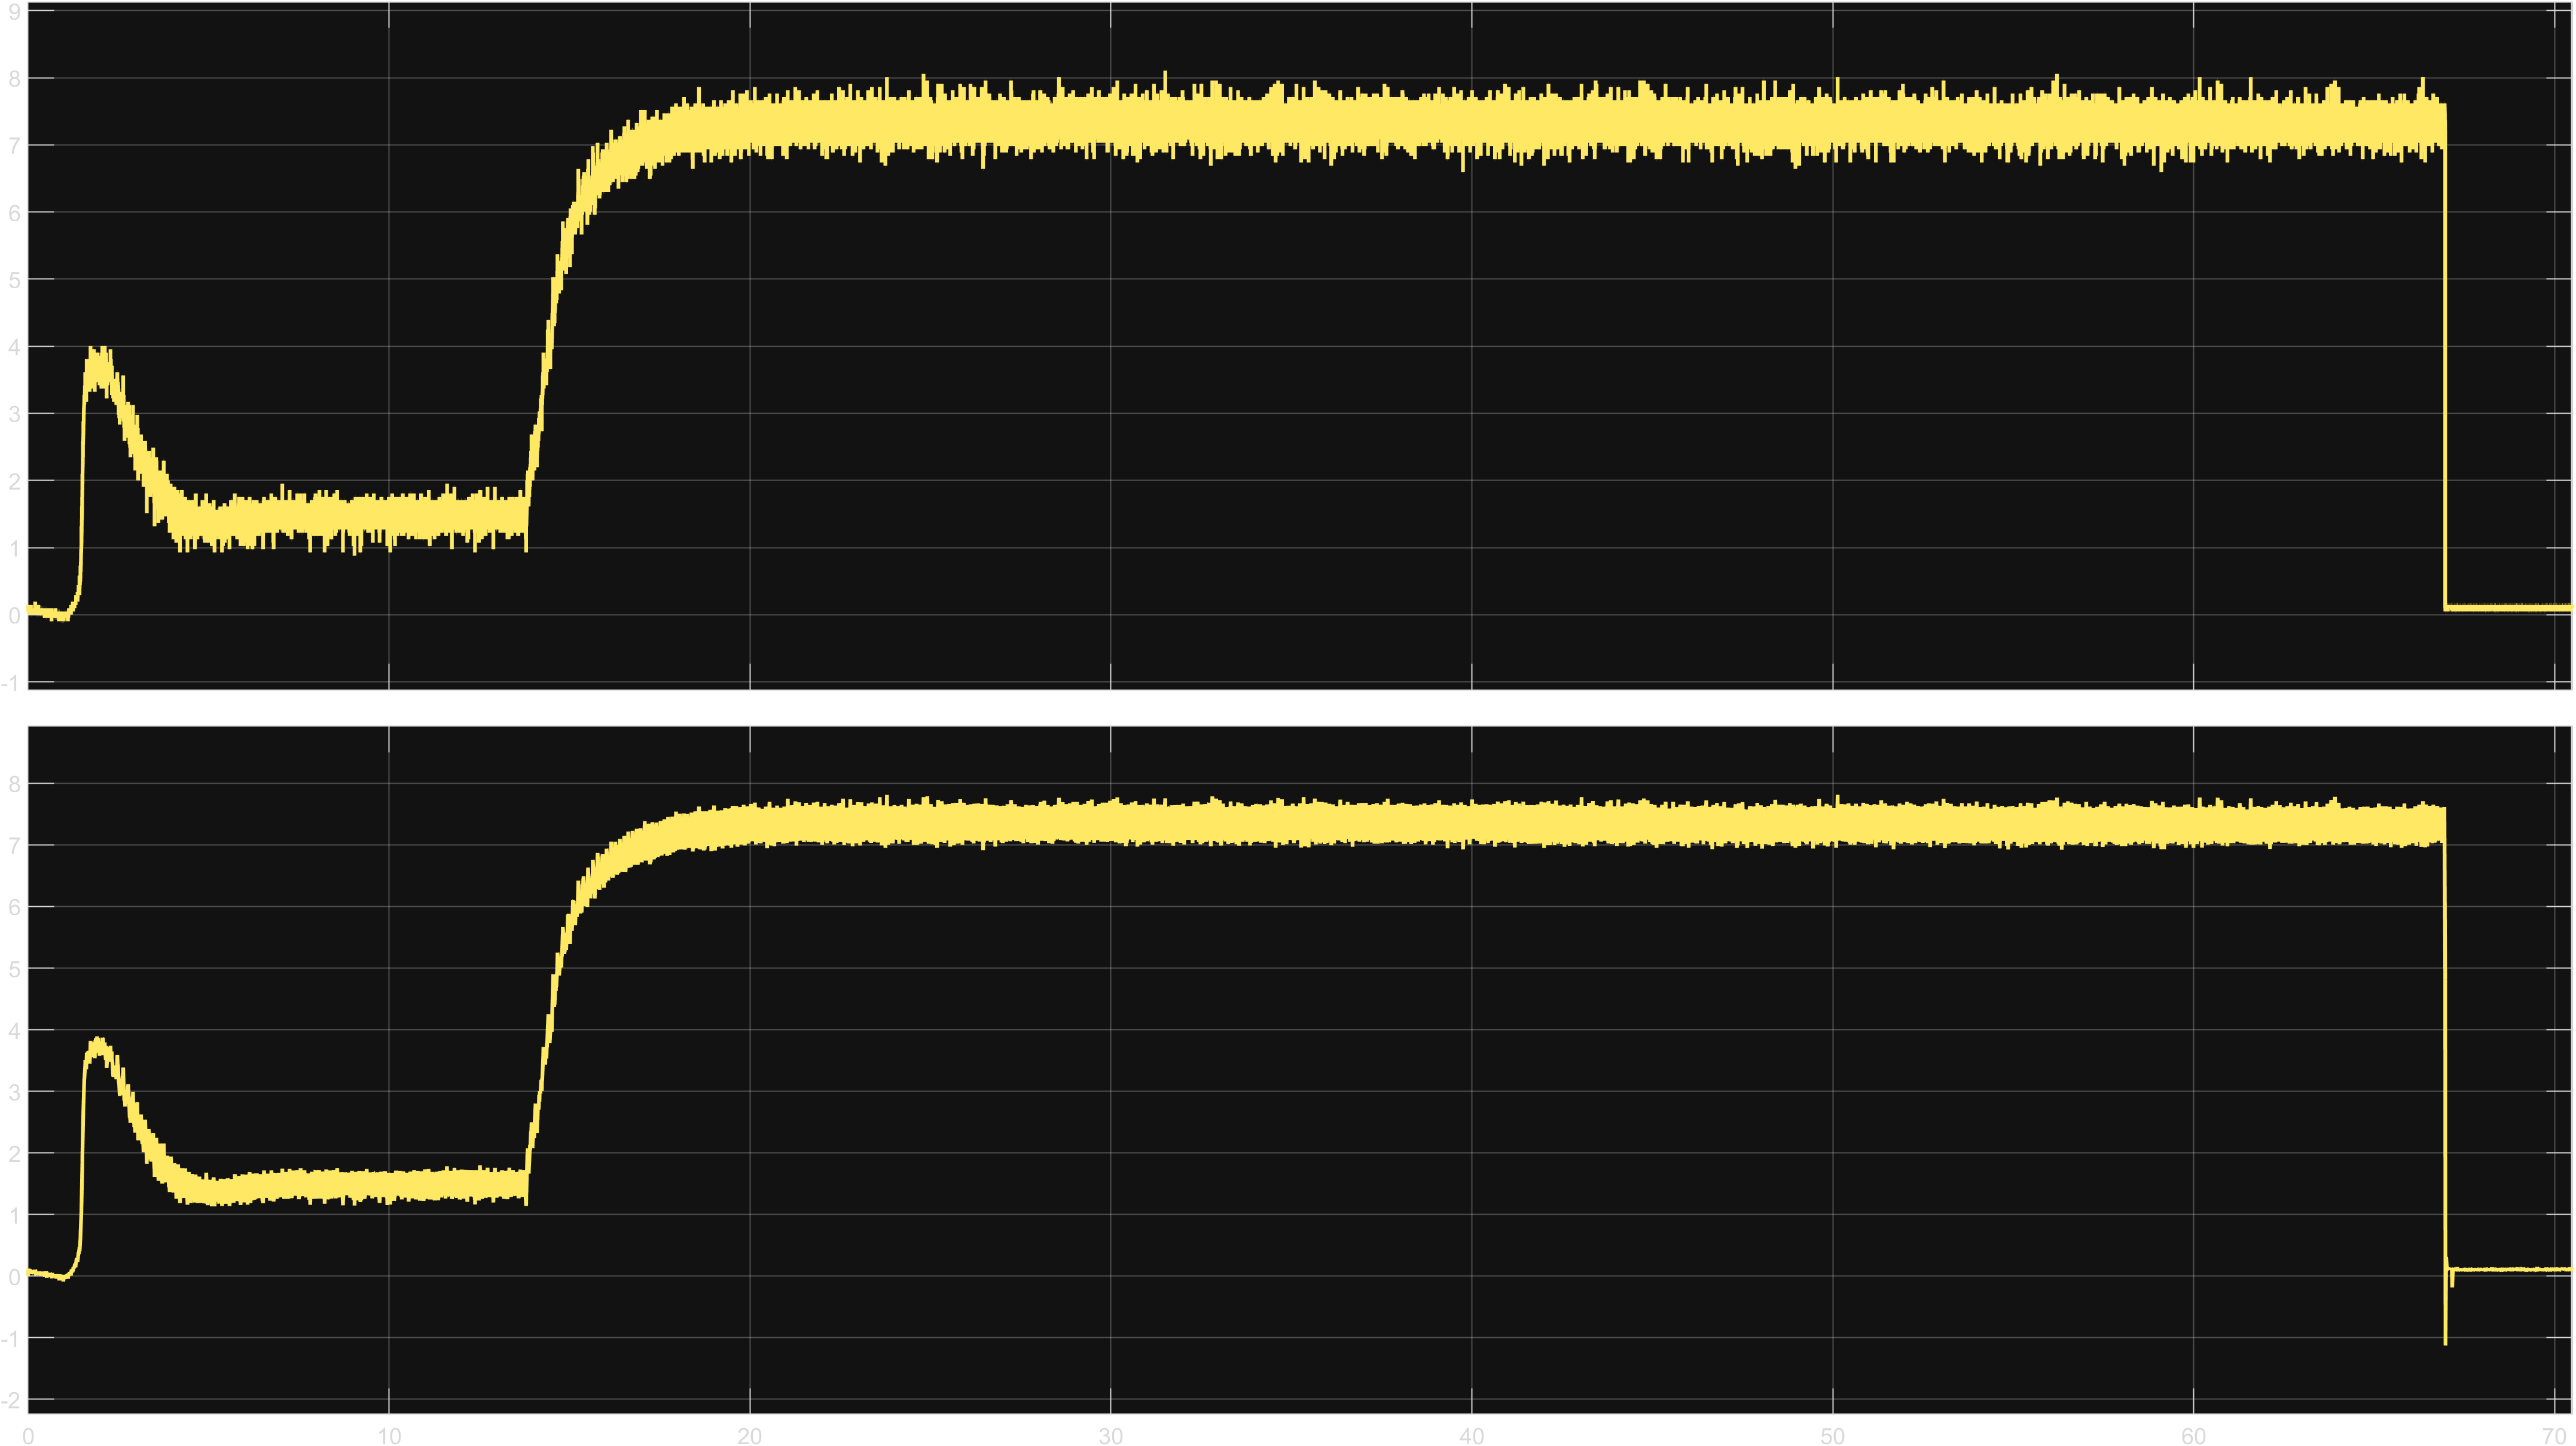
\includegraphics[width=\linewidth, keepaspectratio]{figures/p3i.png}
    \vspace{0.5em}
    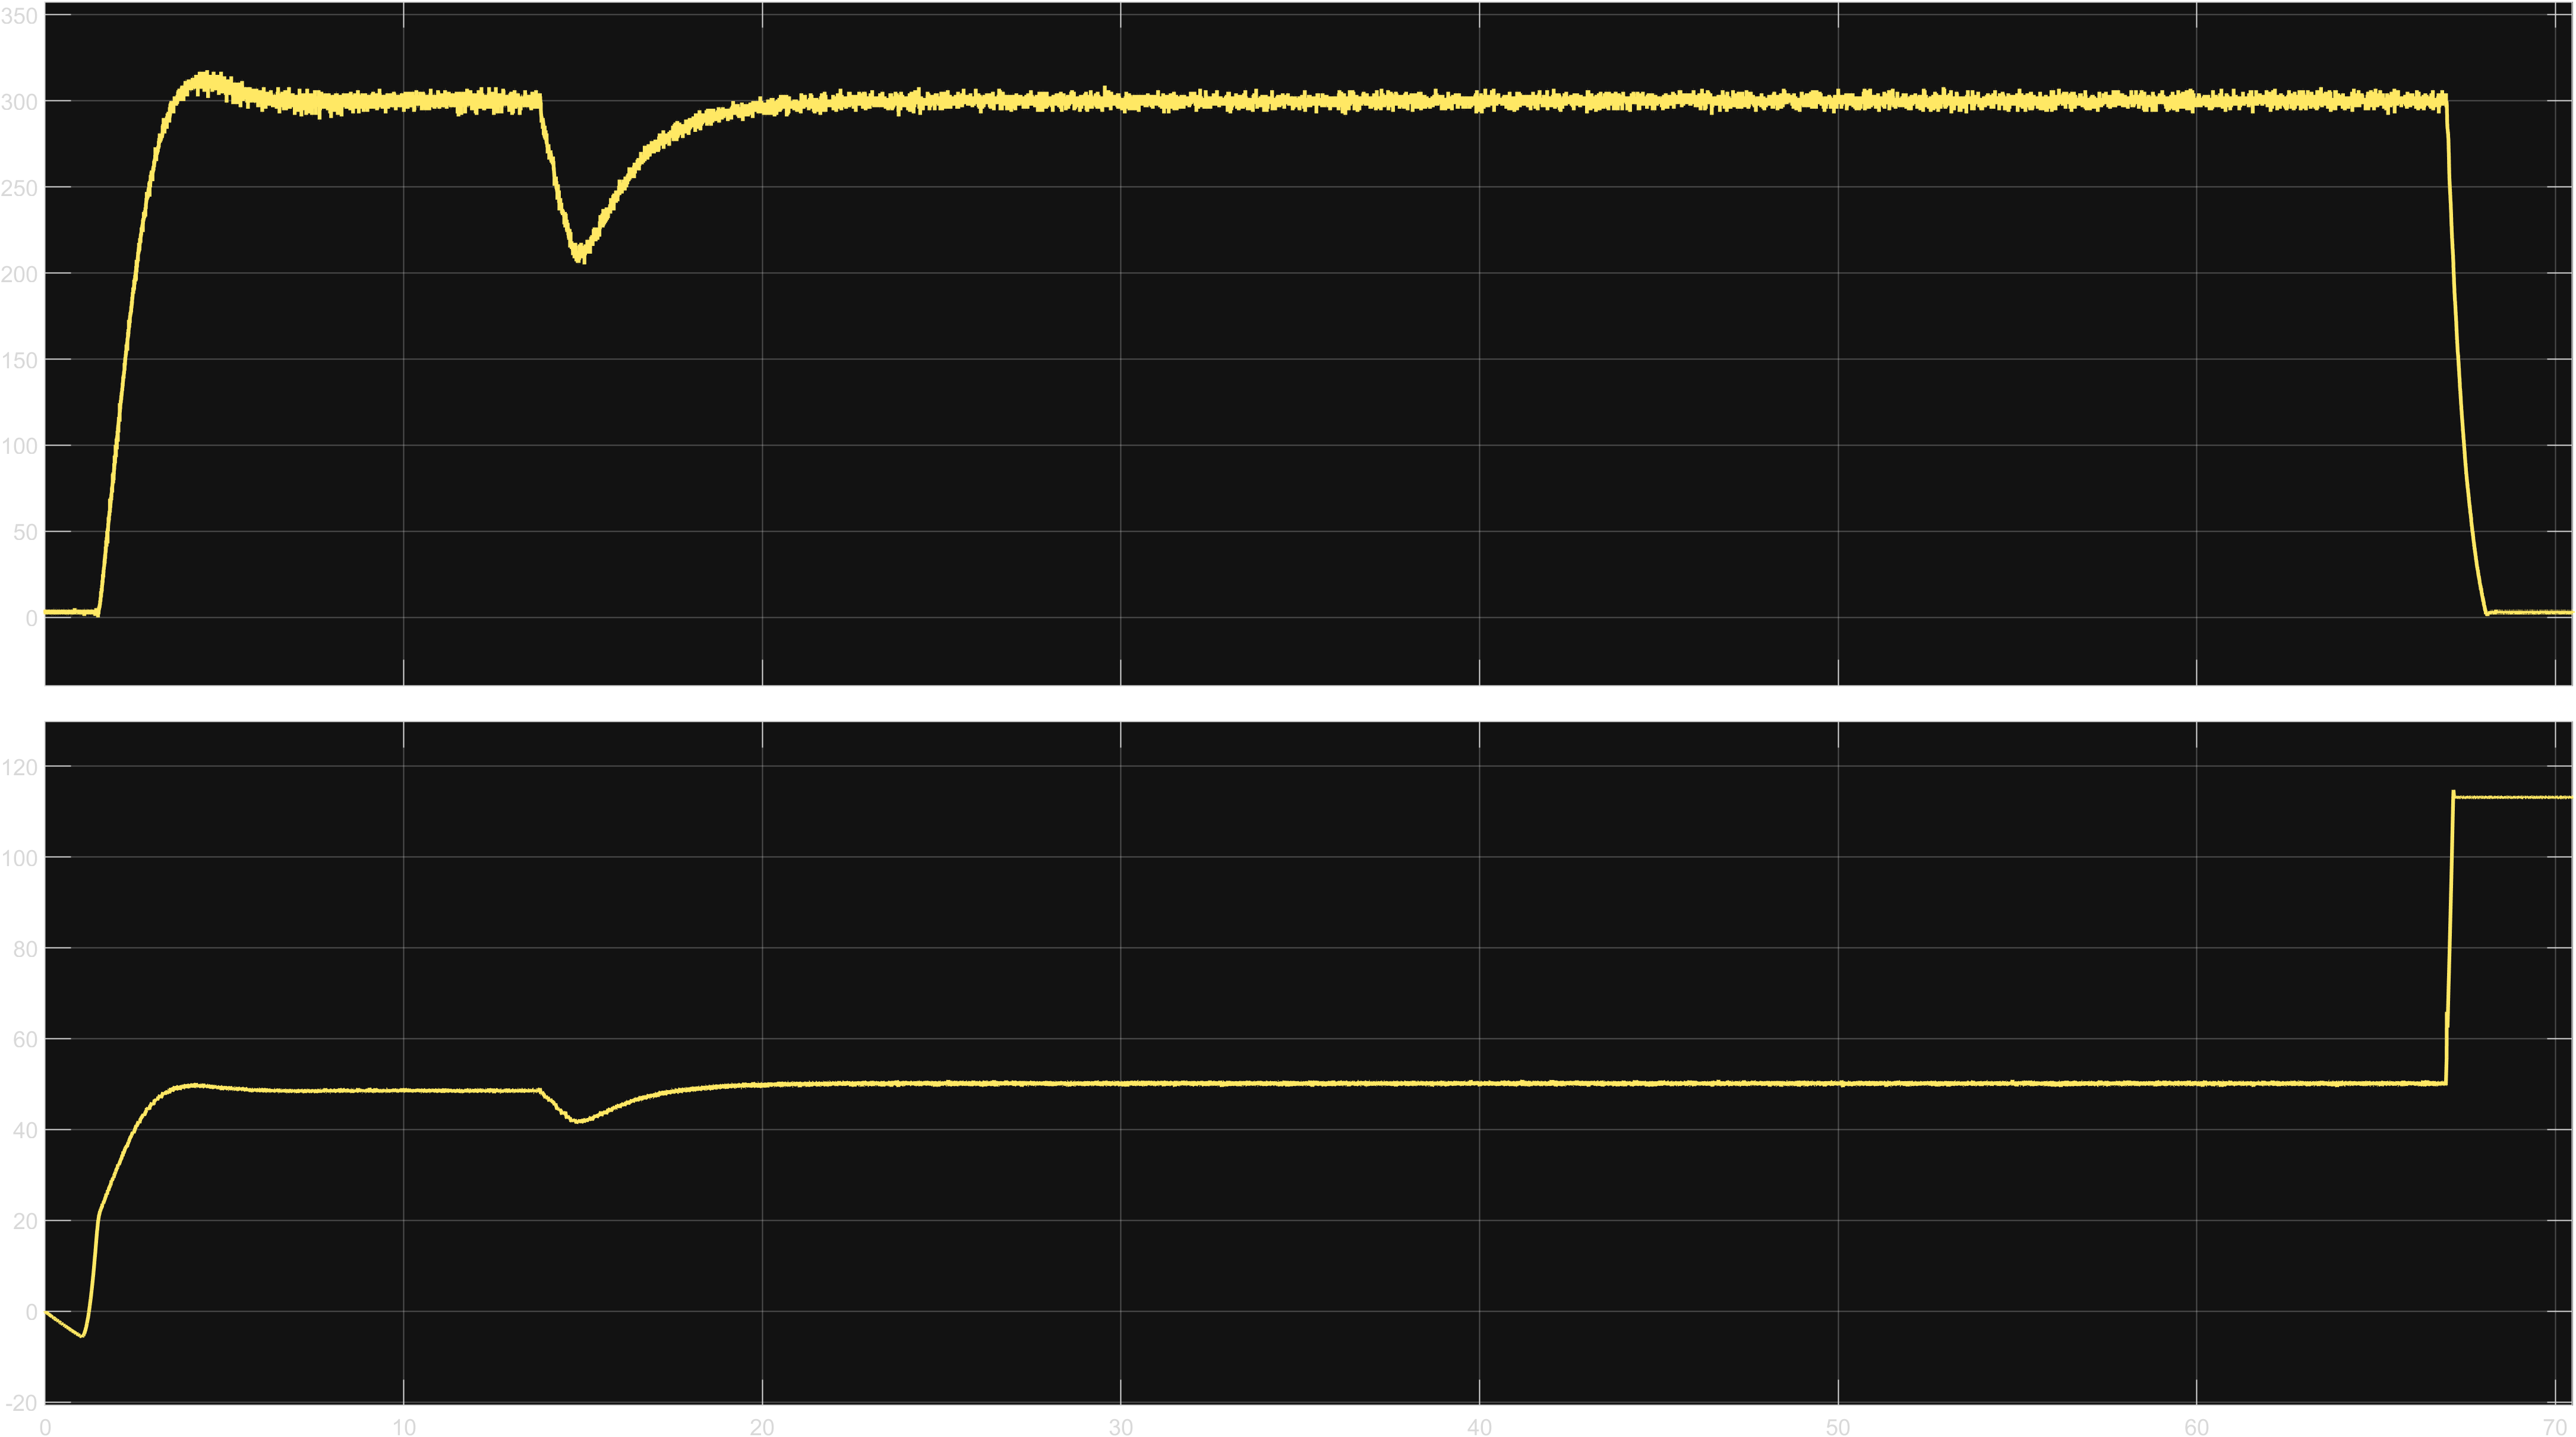
\includegraphics[width=\linewidth, keepaspectratio]{figures/pw.png}
    \caption{Observer validation --- comparison between measured and estimated variables (top: current , bottom: speed).}
    \label{fig:exp_obs_results}
\end{figure}


\newpage
%------------ Conclusion ----------------

\section{Conclusion}
The experimental validation confirmed that the control structures developed in simulation work effectively on the real DC drive, with minor adjustments to account for hardware and safety constraints. 
The current and speed control loops both met the steady-state and dynamic specifications, demonstrating good robustness against disturbances.

The observer-based approach was successful in simulation and partially in the laboratory. 
The current estimation was accurate, but the torque estimation was affected by measurement noise, leading to instability when used for disturbance compensation. 
This highlights the practical challenges of implementing sensorless control on real hardware.

Overall, this practical work successfully connected theoretical modeling, simulation, and experimental implementation. 
It demonstrated the fundamental principles of cascaded control and observer design, and showed how these techniques can be adapted for real-world electrical drives, where nonlinearity, friction, and converter effects must be carefully handled to ensure system stability and precision.





\end{document}